% Options for packages loaded elsewhere
\PassOptionsToPackage{unicode}{hyperref}
\PassOptionsToPackage{hyphens}{url}
\PassOptionsToPackage{dvipsnames,svgnames,x11names}{xcolor}
%
\documentclass[
  letterpaper,
  DIV=11,
  numbers=noendperiod]{scrreprt}

\usepackage{amsmath,amssymb}
\usepackage{iftex}
\ifPDFTeX
  \usepackage[T1]{fontenc}
  \usepackage[utf8]{inputenc}
  \usepackage{textcomp} % provide euro and other symbols
\else % if luatex or xetex
  \usepackage{unicode-math}
  \defaultfontfeatures{Scale=MatchLowercase}
  \defaultfontfeatures[\rmfamily]{Ligatures=TeX,Scale=1}
\fi
\usepackage{lmodern}
\ifPDFTeX\else  
    % xetex/luatex font selection
\fi
% Use upquote if available, for straight quotes in verbatim environments
\IfFileExists{upquote.sty}{\usepackage{upquote}}{}
\IfFileExists{microtype.sty}{% use microtype if available
  \usepackage[]{microtype}
  \UseMicrotypeSet[protrusion]{basicmath} % disable protrusion for tt fonts
}{}
\makeatletter
\@ifundefined{KOMAClassName}{% if non-KOMA class
  \IfFileExists{parskip.sty}{%
    \usepackage{parskip}
  }{% else
    \setlength{\parindent}{0pt}
    \setlength{\parskip}{6pt plus 2pt minus 1pt}}
}{% if KOMA class
  \KOMAoptions{parskip=half}}
\makeatother
\usepackage{xcolor}
\setlength{\emergencystretch}{3em} % prevent overfull lines
\setcounter{secnumdepth}{5}
% Make \paragraph and \subparagraph free-standing
\makeatletter
\ifx\paragraph\undefined\else
  \let\oldparagraph\paragraph
  \renewcommand{\paragraph}{
    \@ifstar
      \xxxParagraphStar
      \xxxParagraphNoStar
  }
  \newcommand{\xxxParagraphStar}[1]{\oldparagraph*{#1}\mbox{}}
  \newcommand{\xxxParagraphNoStar}[1]{\oldparagraph{#1}\mbox{}}
\fi
\ifx\subparagraph\undefined\else
  \let\oldsubparagraph\subparagraph
  \renewcommand{\subparagraph}{
    \@ifstar
      \xxxSubParagraphStar
      \xxxSubParagraphNoStar
  }
  \newcommand{\xxxSubParagraphStar}[1]{\oldsubparagraph*{#1}\mbox{}}
  \newcommand{\xxxSubParagraphNoStar}[1]{\oldsubparagraph{#1}\mbox{}}
\fi
\makeatother

\usepackage{color}
\usepackage{fancyvrb}
\newcommand{\VerbBar}{|}
\newcommand{\VERB}{\Verb[commandchars=\\\{\}]}
\DefineVerbatimEnvironment{Highlighting}{Verbatim}{commandchars=\\\{\}}
% Add ',fontsize=\small' for more characters per line
\usepackage{framed}
\definecolor{shadecolor}{RGB}{241,243,245}
\newenvironment{Shaded}{\begin{snugshade}}{\end{snugshade}}
\newcommand{\AlertTok}[1]{\textcolor[rgb]{0.68,0.00,0.00}{#1}}
\newcommand{\AnnotationTok}[1]{\textcolor[rgb]{0.37,0.37,0.37}{#1}}
\newcommand{\AttributeTok}[1]{\textcolor[rgb]{0.40,0.45,0.13}{#1}}
\newcommand{\BaseNTok}[1]{\textcolor[rgb]{0.68,0.00,0.00}{#1}}
\newcommand{\BuiltInTok}[1]{\textcolor[rgb]{0.00,0.23,0.31}{#1}}
\newcommand{\CharTok}[1]{\textcolor[rgb]{0.13,0.47,0.30}{#1}}
\newcommand{\CommentTok}[1]{\textcolor[rgb]{0.37,0.37,0.37}{#1}}
\newcommand{\CommentVarTok}[1]{\textcolor[rgb]{0.37,0.37,0.37}{\textit{#1}}}
\newcommand{\ConstantTok}[1]{\textcolor[rgb]{0.56,0.35,0.01}{#1}}
\newcommand{\ControlFlowTok}[1]{\textcolor[rgb]{0.00,0.23,0.31}{\textbf{#1}}}
\newcommand{\DataTypeTok}[1]{\textcolor[rgb]{0.68,0.00,0.00}{#1}}
\newcommand{\DecValTok}[1]{\textcolor[rgb]{0.68,0.00,0.00}{#1}}
\newcommand{\DocumentationTok}[1]{\textcolor[rgb]{0.37,0.37,0.37}{\textit{#1}}}
\newcommand{\ErrorTok}[1]{\textcolor[rgb]{0.68,0.00,0.00}{#1}}
\newcommand{\ExtensionTok}[1]{\textcolor[rgb]{0.00,0.23,0.31}{#1}}
\newcommand{\FloatTok}[1]{\textcolor[rgb]{0.68,0.00,0.00}{#1}}
\newcommand{\FunctionTok}[1]{\textcolor[rgb]{0.28,0.35,0.67}{#1}}
\newcommand{\ImportTok}[1]{\textcolor[rgb]{0.00,0.46,0.62}{#1}}
\newcommand{\InformationTok}[1]{\textcolor[rgb]{0.37,0.37,0.37}{#1}}
\newcommand{\KeywordTok}[1]{\textcolor[rgb]{0.00,0.23,0.31}{\textbf{#1}}}
\newcommand{\NormalTok}[1]{\textcolor[rgb]{0.00,0.23,0.31}{#1}}
\newcommand{\OperatorTok}[1]{\textcolor[rgb]{0.37,0.37,0.37}{#1}}
\newcommand{\OtherTok}[1]{\textcolor[rgb]{0.00,0.23,0.31}{#1}}
\newcommand{\PreprocessorTok}[1]{\textcolor[rgb]{0.68,0.00,0.00}{#1}}
\newcommand{\RegionMarkerTok}[1]{\textcolor[rgb]{0.00,0.23,0.31}{#1}}
\newcommand{\SpecialCharTok}[1]{\textcolor[rgb]{0.37,0.37,0.37}{#1}}
\newcommand{\SpecialStringTok}[1]{\textcolor[rgb]{0.13,0.47,0.30}{#1}}
\newcommand{\StringTok}[1]{\textcolor[rgb]{0.13,0.47,0.30}{#1}}
\newcommand{\VariableTok}[1]{\textcolor[rgb]{0.07,0.07,0.07}{#1}}
\newcommand{\VerbatimStringTok}[1]{\textcolor[rgb]{0.13,0.47,0.30}{#1}}
\newcommand{\WarningTok}[1]{\textcolor[rgb]{0.37,0.37,0.37}{\textit{#1}}}

\providecommand{\tightlist}{%
  \setlength{\itemsep}{0pt}\setlength{\parskip}{0pt}}\usepackage{longtable,booktabs,array}
\usepackage{calc} % for calculating minipage widths
% Correct order of tables after \paragraph or \subparagraph
\usepackage{etoolbox}
\makeatletter
\patchcmd\longtable{\par}{\if@noskipsec\mbox{}\fi\par}{}{}
\makeatother
% Allow footnotes in longtable head/foot
\IfFileExists{footnotehyper.sty}{\usepackage{footnotehyper}}{\usepackage{footnote}}
\makesavenoteenv{longtable}
\usepackage{graphicx}
\makeatletter
\newsavebox\pandoc@box
\newcommand*\pandocbounded[1]{% scales image to fit in text height/width
  \sbox\pandoc@box{#1}%
  \Gscale@div\@tempa{\textheight}{\dimexpr\ht\pandoc@box+\dp\pandoc@box\relax}%
  \Gscale@div\@tempb{\linewidth}{\wd\pandoc@box}%
  \ifdim\@tempb\p@<\@tempa\p@\let\@tempa\@tempb\fi% select the smaller of both
  \ifdim\@tempa\p@<\p@\scalebox{\@tempa}{\usebox\pandoc@box}%
  \else\usebox{\pandoc@box}%
  \fi%
}
% Set default figure placement to htbp
\def\fps@figure{htbp}
\makeatother
% definitions for citeproc citations
\NewDocumentCommand\citeproctext{}{}
\NewDocumentCommand\citeproc{mm}{%
  \begingroup\def\citeproctext{#2}\cite{#1}\endgroup}
\makeatletter
 % allow citations to break across lines
 \let\@cite@ofmt\@firstofone
 % avoid brackets around text for \cite:
 \def\@biblabel#1{}
 \def\@cite#1#2{{#1\if@tempswa , #2\fi}}
\makeatother
\newlength{\cslhangindent}
\setlength{\cslhangindent}{1.5em}
\newlength{\csllabelwidth}
\setlength{\csllabelwidth}{3em}
\newenvironment{CSLReferences}[2] % #1 hanging-indent, #2 entry-spacing
 {\begin{list}{}{%
  \setlength{\itemindent}{0pt}
  \setlength{\leftmargin}{0pt}
  \setlength{\parsep}{0pt}
  % turn on hanging indent if param 1 is 1
  \ifodd #1
   \setlength{\leftmargin}{\cslhangindent}
   \setlength{\itemindent}{-1\cslhangindent}
  \fi
  % set entry spacing
  \setlength{\itemsep}{#2\baselineskip}}}
 {\end{list}}
\usepackage{calc}
\newcommand{\CSLBlock}[1]{\hfill\break\parbox[t]{\linewidth}{\strut\ignorespaces#1\strut}}
\newcommand{\CSLLeftMargin}[1]{\parbox[t]{\csllabelwidth}{\strut#1\strut}}
\newcommand{\CSLRightInline}[1]{\parbox[t]{\linewidth - \csllabelwidth}{\strut#1\strut}}
\newcommand{\CSLIndent}[1]{\hspace{\cslhangindent}#1}

\KOMAoption{captions}{tableheading}
\makeatletter
\@ifpackageloaded{bookmark}{}{\usepackage{bookmark}}
\makeatother
\makeatletter
\@ifpackageloaded{caption}{}{\usepackage{caption}}
\AtBeginDocument{%
\ifdefined\contentsname
  \renewcommand*\contentsname{Table of contents}
\else
  \newcommand\contentsname{Table of contents}
\fi
\ifdefined\listfigurename
  \renewcommand*\listfigurename{List of Figures}
\else
  \newcommand\listfigurename{List of Figures}
\fi
\ifdefined\listtablename
  \renewcommand*\listtablename{List of Tables}
\else
  \newcommand\listtablename{List of Tables}
\fi
\ifdefined\figurename
  \renewcommand*\figurename{Figure}
\else
  \newcommand\figurename{Figure}
\fi
\ifdefined\tablename
  \renewcommand*\tablename{Table}
\else
  \newcommand\tablename{Table}
\fi
}
\@ifpackageloaded{float}{}{\usepackage{float}}
\floatstyle{ruled}
\@ifundefined{c@chapter}{\newfloat{codelisting}{h}{lop}}{\newfloat{codelisting}{h}{lop}[chapter]}
\floatname{codelisting}{Listing}
\newcommand*\listoflistings{\listof{codelisting}{List of Listings}}
\makeatother
\makeatletter
\makeatother
\makeatletter
\@ifpackageloaded{caption}{}{\usepackage{caption}}
\@ifpackageloaded{subcaption}{}{\usepackage{subcaption}}
\makeatother

\usepackage{bookmark}

\IfFileExists{xurl.sty}{\usepackage{xurl}}{} % add URL line breaks if available
\urlstyle{same} % disable monospaced font for URLs
\hypersetup{
  pdftitle={Social Network Analysis: A Guide Using Principles of the ADAPT Model},
  pdfauthor={Tom R. Leppard},
  colorlinks=true,
  linkcolor={blue},
  filecolor={Maroon},
  citecolor={Blue},
  urlcolor={Blue},
  pdfcreator={LaTeX via pandoc}}


\title{Social Network Analysis: A Guide Using Principles of the ADAPT
Model}
\author{Tom R. Leppard}
\date{2025-05-16}

\begin{document}
\maketitle

\renewcommand*\contentsname{Table of contents}
{
\hypersetup{linkcolor=}
\setcounter{tocdepth}{2}
\tableofcontents
}

\bookmarksetup{startatroot}

\chapter*{Preface}\label{preface}
\addcontentsline{toc}{chapter}{Preface}

\markboth{Preface}{Preface}

This book is designed to build skills in Social Network Analysis by
teaching it using principles from the data science teaching and learning
model called ADAPT. It is designed to demonstrate principles of the
model and will discuss aspects aspect of the model (learn more in
\href{intro.qmd}{Chapter 2}).

The book is divided into three sections that mirror the units of the
course. Each chapter of the book with take you through a data science
workflow session-by-session bulding from data cleaning to analysis.
First, it starts building your skills cleaning and transforming network
data. In this unit you will be learning about network data structured,
bringing network data into R and best practices for cleaning network
data. Second, it transitions into a unit on network visualisation. This
unit builds your skills in basic, intermediate, and advanced network
visualisation. The aim of this unit is to help you create clean network
visualisations that tell a clear story, and engage your viewers.
Finally, the book finishes with some modules on analysing network data.
Specifically, a discussion on the units of network analysis, individuals
(nodes in the networks), communities (clusters of nodes in the
networks), and the network itself. There is much to learn beyond this
book, however, by the end of this you will have learned the fundamental
principles and will build competence in network analysis.

Enjoy!

\section*{Attribution}\label{attribution}
\addcontentsline{toc}{section}{Attribution}

\markright{Attribution}

\textbf{License}

This book is licensed under a Creative Commons
Attribution-\href{https://creativecommons.org/licenses/by-nc-nd/4.0/}{NonCommercial-NoDerivatives
4.0 International License (CC BY-NC-ND 4.0).}

You may share this material in any medium or format for noncommercial
purposes, provided you give appropriate credit, do not modify the
material, and do not use it for commercial purposes.

\pandocbounded{
\includegraphics[keepaspectratio]{creative commons.png}}

\textbf{Suggested Citation}

Leppard, Tom R. \emph{Social Network Analysis: A Guide Using Principles
of the ADAPT Model}. 2025. Available at:
\url{https://tom-r-leppard.github.io/SP25_SNA_Book/}

\part{Introduction and Getting Going}

\chapter{On The ADAPT Model}\label{on-the-adapt-model}

This book is patterned after the ADAPT model championed by North
Carolina State University's Data Science and AI Academy (DSA). This
\href{https://datascienceacademy.ncsu.edu/courses/course-model/}{model}
stands for All-campus Data science and AI through Project based Teaching
and learning. This model serves as a framework for the workflow of this
book and it's pedagogical ethos.

For a little context, all instructors at the Data Science and AI Academy
are trained to teach using this model. The Academy's data science
courses are open to all students of any discipline and professional
stage. Students include undergraduate, graduate university attendees as
well as staff, faculty, and community members. With such a diverse
student body, the DSA uses the ADAPT teaching model to create a
consistent form of instruction across all courses. In a way, the
teaching model threads all students together, weaving their experiences
into a cohesive experience across any course that students take.

At its core, the model is designed to make computational skills
accessible to everyone, regardless of their discipline. It emphasises
student agency as much as possible within the confines of the unique
course objectives. For example, students are encouraged to select their
own dataset to use for their final project based on their interests.
Instructors are guided to introduce their students to different datasets
and techniques to appeal to student-interests.

In this spirit of this model, you'll see that I use some fun data (e.g.,
Harry Potter, UK Grime music, etc.) to teach network principles and R
skills. I find these appeal to a very broad student body. I also teach
based on concepts more than explaining code. Understanding the `what'
and the `why' behind social network analysis more than explaining every
syntactical function, I find, facilitates learning for many. For
students more interested in the nature of the code or the mathematics
behind the measurements, I extend more resources on an individual basis.
Therefore, this book, presented as a course, serves as a great
introduction for students to social networks and instructors to the
ADAPT teaching and learning approach.

\section{ADAPT for Instructors}\label{adapt-for-instructors}

The teaching model is a living document that the Data Science and AI
team, headed by Rachel Levy, are constantly working on. As previously
mentioned, the students are at the core of this model as is the belief
of the DSA that data science acumen can be taught to people from every
disciplinary background. In fact, it behooves all to engage with data
and become data literate (understanding how to interpret data) in a
data-driven world!

I do not go into detail here but suffice it to say that the ADAPT model
comprises three parts:

\begin{enumerate}
\def\labelenumi{\arabic{enumi}.}
\item
  Project-based Learning
\item
  10 Common Learning Elements
\item
  Workforce Preparedness
\end{enumerate}

\begin{figure}[H]

{\centering \pandocbounded{
\includegraphics[keepaspectratio]{ADAPT - ICON.png}}

}

\caption{ADAPT Model Icon - DSA}

\end{figure}%

This book was created from a course taught at the DSA under the
direction of the ADAPT model. It's goal is not to serve as an exemplar
of the model, but rather to encourage instructors to engage with the
``spirit'' of the model. Consider teaching project-based courses that
centres the interests of your students - maximising their agency.
Further, consider teaching computational skills in such a way as to open
its content to all interested parties.

Each of the units and modules in this book are designed with students in
mind. I discuss each elements of the ADAPT model in the Unit
introduction chapters. The purpose of this book is to enact these
principles and enable other instructors wishing to teach social network
analysis to do the same. All data used in this book is available using
the ``ADAPTSNA'' R package. Alternatively, you may wish to use other
data and just use this guide to inform your own syllabus and activities.

Finally, let me point you to the assignments in this course. You are
welcome to use or to change these assignments as you wish. They are
designed to build a student's skills throughout the semester as they
progress towards their final project. Courses taught using the ADAPT
model do not have quizzes or tests, but rather scaffold multiple
assignments throughout the semester aimed at building a capstone project
at the end of the course. This scaffolding approach enables the student
to build their progress continually and the assignments serve as
milestones in their progress. The material in this book is designed to
fill a 1 credit-hour course. If yours is a longer course, you may wish
to alter the pacing of the semester adding or rearranging the content of
this course. Regardless here is a little insight into the assignments I
use and why I think these milestones are useful to the student's success
and for you to grade the student.

\begin{enumerate}
\def\labelenumi{\arabic{enumi}.}
\item
  \href{A1_My\%20Ego\%20Network.qmd}{Assignment 1} (10 marks) acts as an
  orientation to network principles and parlance. This, no-tech/low-tech
  assignments sees students create an ego-network, their ego-network
  teaching them the vocabulary of network analysis.
\item
  \href{A2_Project\%20Prospectus.qmd}{Assignment 2} (10 marks) is the
  first milestone of their project. This no-tech assignment sees
  students present ideas for their final project encouraging them to
  present two separate ideas for datasets once they have either looked
  through the GitHub repository or discovered their own dataset. This
  serves as the beginning of a discussion between the instructor and
  student to guide their final project.
\item
  \href{A3_Data_Exploration.qmd}{Assignment 3} (20 marks) is the second
  milestone of their project. This is designed to help students bring
  their data into R, describe it, and suggest any cleaning that they may
  need to do. By this point, they are encouraged to select their data
  that they are going to use.This is an opportunity for the instructor
  to give more in-depth feedback on the data they are using and suggest
  further transformations that they may need.
\item
  \href{A4_Visualisations.qmd}{Assignment 4} (20 marks) is the third
  milestone of their project. This is an opportunity for instructors to
  provide guidance on producing useful visualisations.
\item
  \href{Final\%20Project\%20Instructions.qmd}{The Final Project} (40
  marks) is the last milestone of their project. This an exploratory
  data analysis where students learn to use their exploratory
  visualisations and transformations to form and answer questions about
  their network.
\end{enumerate}

\section{ADAPT for Students}\label{adapt-for-students}

Students, the biggest thing you need to know is that you will be working
on a project for the duration of the course. For more details see
\href{Final\%20Project\%20Instructions.qmd}{the Final Project
Instructions}.

Each unit and assignment is a milestone in your project development. For
this project, you may select any social network data that appeals to
you. I have collated quite a few from various sources available on the
\href{https://github.com/Tom-R-Leppard/SP25_SNA_Book/tree/main/Social\%20Network\%20Analysis\%20-\%20Data}{Github
repo}. Alternatively, you may wish to explore other network data (from
places like the \href{https://networkrepository.com/index.php}{network
repository}, \href{https://www.kaggle.com/}{Kaggle} or others).

Any data that you use, make sure you cite where you are using it from!

\textbf{Pay attention to the introductions of each unit. There are
learning objectives, project milestones, and tips for preparing to do
this professionally.}

\chapter{Getting Started with R}\label{getting-started-with-r}

\section{Quick Start}\label{quick-start}

If you are an old hand when it comes to coding and have experience with
R, great! Know that we will mostly be using the package `igraph' so go
ahead and install it now (you can use the code below). Keep an eye out
for the new packages we use throughout the book and install them as you
go.

The data we will be using come from the ``ADAPTSNA'' package which is
the companion package to this book and available on my Github. Install
it using the code below.

Other than that, get going!

\begin{Shaded}
\begin{Highlighting}[]
\CommentTok{\# Network Package}
\FunctionTok{install.packages}\NormalTok{(}\StringTok{"igraph"}\NormalTok{)}
\FunctionTok{library}\NormalTok{(igraph)}

\CommentTok{\# Package to access data}
\CommentTok{\# Make sure you have remotes installed first}
\FunctionTok{install.packages}\NormalTok{(}\StringTok{"remotes"}\NormalTok{)}
\NormalTok{remotes}\SpecialCharTok{::}\FunctionTok{install\_github}\NormalTok{(}\StringTok{"Tom{-}R{-}Leppard/ADAPTSNA"}\NormalTok{)}
\FunctionTok{library}\NormalTok{(ADAPTSNA)}
\end{Highlighting}
\end{Shaded}

\section{New to R?}\label{new-to-r}

If you are new to R or new to coding, wonderful! This is a great way to
start getting into it. There are a few steps we need to take before you
install the package above. If you are planning on using R long term, I
strongly suggest downloading it and RStudio to your personal machine.
Even if you don't I suggest doing this because it is the most
straightforward (go to option 1). If not, say you don't have a personal
machine and need to use a public machine or one in a lab, then there are
ways to work with that (go to option 2).

\section{Option 1: Downloading
R/RStudio}\label{option-1-downloading-rrstudio}

To get going, you will need to download both R and RStudio. Yes, these
are separate downloads. Think of R as the engine, and Rstudio as the car
you are driving. RStudio makes it easy to do the things you want to do
while R, (the `engine') actually drives everything you do. To do this,
follow the instructions on the
\href{https://posit.co/download/rstudio-desktop/}{Posit} website. At the
time of the publication of this book, this link has 2 steps, one to
install R and the other to install RStudio. Depending on your machine
(if you have a windows, mac or an operating system like Linux) there are
different instructions. Download and install the the ones you need.

\section{Option 2: Posit Cloud}\label{option-2-posit-cloud}

If you do not want to or cannot download R/RStudio, there are a few ways
to use it for free, albeit limited, online. Consider making a free
account on
\href{https://login.posit.cloud/login?redirect=\%2Foauth\%2Fauthorize\%3Fredirect_uri\%3Dhttps\%253A\%252F\%252Fposit.cloud\%252Flogin\%26client_id\%3Dposit-cloud\%26response_type\%3Dcode\%26show_auth\%3D0&product=cloud}{Posit
Cloud}.

Once you have made your account, click on the tab at the top right to
create a new project. Select RStudio. From here on its mostly the same
with a few tweaks, pay attention below for a few differences between
posit cloud and downloading RStudio.

\section{A little about RStudio}\label{a-little-about-rstudio}

Once you have installed it, or created your new project on Posit Cloud,
go ahead and open RStudio. When you open RStudio, you will see four
windows, let's walk through those for a moment. There are multiple uses
for each window. However, for now, we will discuss them how we will be
using them just to get you started.

\begin{enumerate}
\def\labelenumi{\arabic{enumi}.}
\item
  Starting from the top left, you have a window for your script files.
  Think of this as a place to write, run, and store code. Here, you can
  open different files including script, markdown, quarto and others.
  For the sake of what we are doing in this book, just focus on those
  three types.
\item
  On the bottom left there is a space for you to enter code and run it
  directly. This is basically a window to look at the engine.
\item
  Next, the top right window houses your global environment. Think of
  this as a bucket. What you do in the script or the console can fill
  things into the bucket. For example, you can bring in network data and
  store it in this environment.
\item
  Finally, on the bottom right there are multiple reasons we use this
  window. Mostly, the network visualisations we will create will appear
  in the `Plots' or `Viewer' tab.
\end{enumerate}

\subsection{On Packages}\label{on-packages}

Another thing you need to know is that we will be using multiple types
of commands throughout this book. These are grouped into what are called
`packages.' Think of packages as mini dictionaries for different
languages. In this case, however, these languages enable you to do
different things with/to your data.

To access these packages, you first need to install them. You can do
this, using the following function.

\begin{Shaded}
\begin{Highlighting}[]
\FunctionTok{install.packages}\NormalTok{(}\StringTok{"igraph"}\NormalTok{)}
\end{Highlighting}
\end{Shaded}

The above code will download the package to your machine (or your
project space on posit.cloud). Then, you need to tell R which
``language'' you are coding in each time you open up RStudio. To do
this, you use the `library()' function. Keep an eye out for the various
packages use. If you see a command to bring in a package you don't
recognise, you will need to install it (just replace igraph with the
name of the other package in the above chunk).

\begin{Shaded}
\begin{Highlighting}[]
\FunctionTok{library}\NormalTok{(igraph)}
\end{Highlighting}
\end{Shaded}

You only ever need to install it once on to your machine but every time
you open R you will need to activate it in your library.

\subsection{Loading Data}\label{loading-data}

Great stuff! You now have RStudio sorted out and you (if you ran the
above) have installed igraph. Now, the last thing you need is the data
that you are going to use and to bring it into the environment. There
are many ways that you can do this, but I have provided you, what I
think, is the simplest low-tech method that you can use across both on
posit cloud or your own machine.

In each of the chapters, you will need both the ``igraph'' and
``ADAPTSNA'' packages. ``igraph'' is the network package, ``ADAPTSNA''
is a package to help you bring in the data used in this book. Follow the
code below to install the second package.

\begin{Shaded}
\begin{Highlighting}[]
\CommentTok{\# Package to access data}
\CommentTok{\# Make sure you have remotes installed first}
\FunctionTok{install.packages}\NormalTok{(}\StringTok{"remotes"}\NormalTok{)}
\NormalTok{remotes}\SpecialCharTok{::}\FunctionTok{install\_github}\NormalTok{(}\StringTok{"Tom{-}R{-}Leppard/ADAPTSNA"}\NormalTok{)}
\FunctionTok{library}\NormalTok{(ADAPTSNA)}
\end{Highlighting}
\end{Shaded}

This package has all of the datasets we will be using for this book. To
see all of the available datasets in this package, use the code below.
This will return the names of the .csv files we are using.

\begin{Shaded}
\begin{Highlighting}[]
\FunctionTok{list\_data\_files}\NormalTok{()}
\end{Highlighting}
\end{Shaded}

The only thing left to do, is to head over to the
\href{https://github.com/Tom-R-Leppard/SP25_SNA_Book/tree/main/Social\%20Network\%20Analysis\%20-\%20Data}{Github
repo} and get started thinking about your project!

\chapter{Contents and Schedule}\label{contents-and-schedule}

Here is a roadmap for how to use this book.

Depending on your usage, you might wish change the sequencing of the
content of this book. However, it is designed so that each topic can
serve as the content for a week in a semester. The flow of the book
follows the logic of a data science workflow that will help readers flow
from wrangling, visualising and then analysing network data.

\section{Unit 1 - Cleaning and
Transforming}\label{unit-1---cleaning-and-transforming}

\begin{longtable}[]{@{}
  >{\centering\arraybackslash}p{(\linewidth - 4\tabcolsep) * \real{0.1351}}
  >{\centering\arraybackslash}p{(\linewidth - 4\tabcolsep) * \real{0.5068}}
  >{\centering\arraybackslash}p{(\linewidth - 4\tabcolsep) * \real{0.3514}}@{}}
\toprule\noalign{}
\begin{minipage}[b]{\linewidth}\centering
Topic
\end{minipage} & \begin{minipage}[b]{\linewidth}\centering
Chapter
\end{minipage} & \begin{minipage}[b]{\linewidth}\centering
Assignments
\end{minipage} \\
\midrule\noalign{}
\endhead
\bottomrule\noalign{}
\endlastfoot
Introduction & \href{Unit\%201.qmd}{Chapter 4} & \\
Data Structures & \href{Network\%20Data\%20Structures.qmd}{Chapter 5}
& \\
Cleaning \#1 &
\href{Cleaning\%20Network\%20Data\%20-\%20Trimming\%20and\%20Adding.qmd}{Chapter
6} & \href{A1_My\%20Ego\%20Network.qmd}{My Ego Network} \\
Cleaning \#2 &
\href{Cleaning\%20Network\%20Data\%20-\%20Subgraphs.qmd}{Chapter 7} & \\
Attributes & \href{Node\%20and\%20Edge\%20Attributes.qmd}{Chapter 8}
& \\
Two-Mode Networks &
\href{Two\%20Mode\%20Networks\%20-\%20AM.qmd}{Chapter 9}

\href{Two\%20Mode\%20Networks\%20-\%20Edgelists.qmd}{Chapter 10} &
\href{A2_Project\%20Prospectus.qmd}{Project Prospectus} \\
\end{longtable}

\section{Unit 2 - Visualising}\label{unit-2---visualising}

\begin{longtable}[]{@{}
  >{\centering\arraybackslash}p{(\linewidth - 4\tabcolsep) * \real{0.3333}}
  >{\centering\arraybackslash}p{(\linewidth - 4\tabcolsep) * \real{0.3333}}
  >{\centering\arraybackslash}p{(\linewidth - 4\tabcolsep) * \real{0.3333}}@{}}
\toprule\noalign{}
\begin{minipage}[b]{\linewidth}\centering
Topic
\end{minipage} & \begin{minipage}[b]{\linewidth}\centering
Chapter
\end{minipage} & \begin{minipage}[b]{\linewidth}\centering
Assignments
\end{minipage} \\
\midrule\noalign{}
\endhead
\bottomrule\noalign{}
\endlastfoot
Introduction & \href{Unit\%202.qmd}{Chapter 11} & \\
Basic & \href{Basic\%20Visualisation.qmd}{Chapter 12} &
\href{A3_Data\%20Exploration.qmd}{Data Exploration} \\
Intermediate & \href{Intermediate\%20Visualisation.qmd}{Chapter 13} & \\
Advanced \#1 &
\href{Advanced\%20Visualisation\%20-\%20Interactive.qmd}{Chapter 14}
& \\
Advanced \#2 &
\href{Advanced\%20Visualisation\%20-\%20Dynamic.qmd}{Chapter 15} &
\href{A4_Visualisations.qmd}{Visualisation} \\
\end{longtable}

\section{Unit 3 - Analysing}\label{unit-3---analysing}

\begin{longtable}[]{@{}
  >{\centering\arraybackslash}p{(\linewidth - 4\tabcolsep) * \real{0.3333}}
  >{\centering\arraybackslash}p{(\linewidth - 4\tabcolsep) * \real{0.3333}}
  >{\centering\arraybackslash}p{(\linewidth - 4\tabcolsep) * \real{0.3333}}@{}}
\toprule\noalign{}
\begin{minipage}[b]{\linewidth}\centering
Topic
\end{minipage} & \begin{minipage}[b]{\linewidth}\centering
Chapter
\end{minipage} & \begin{minipage}[b]{\linewidth}\centering
Assignments
\end{minipage} \\
\midrule\noalign{}
\endhead
\bottomrule\noalign{}
\endlastfoot
Introduction & \href{Unit\%203.qmd}{Chapter 16} & \\
People & \href{People\%20In\%20Networks.qmd}{Chapter 17} & \\
Communities & \href{Communities\%20in\%20Networks.qmd}{Chapter 18} & \\
Networks & \href{Networks\%20of\%20People.qmd}{Chapter 19} &
\href{Final\%20Project\%20Instructions.qmd}{Final Project} \\
\end{longtable}

\part{Unit 1: Cleaning and Transforming Network Data}

\chapter{Unit 1}\label{unit-1}

\section{Learning Elements}\label{learning-elements}

In this unit, we will cover how to transform and wrangle network data.
Network data aren't always clean. Nor are they always representative of
an entire group. As the researcher, it is up to you to learn best
practices of cleaning your data. It is also important for you to know as
much as possible about the group you are studying. For your research
results to be generalisable to the group you are studying, your data
need to truly represent the group you are studying (whether you have
sample or population data). This process might include trimming or
adding to your network. Or it might include making various subgraphs of
your network.

By the end of this unit you will:

\begin{enumerate}
\def\labelenumi{\arabic{enumi}.}
\item
  Understand how network data is structured
\item
  Know how to bring network data into RStudio
\item
  Clean network data
\item
  Learn the difference between one and two mode networks
\end{enumerate}

\section{Project Milestones}\label{project-milestones}

\begin{longtable}[]{@{}
  >{\raggedright\arraybackslash}p{(\linewidth - 2\tabcolsep) * \real{0.5000}}
  >{\raggedright\arraybackslash}p{(\linewidth - 2\tabcolsep) * \real{0.5000}}@{}}
\toprule\noalign{}
\begin{minipage}[b]{\linewidth}\raggedright
Milestone (assignments linked)
\end{minipage} & \begin{minipage}[b]{\linewidth}\raggedright
Explanation
\end{minipage} \\
\midrule\noalign{}
\endhead
\bottomrule\noalign{}
\endlastfoot
\href{A1_My\%20Ego\%20Network.qmd}{My Ego Network} & Students will draw
their own ego network following an assignment in class. \\
\href{A2_Project\%20Prospectus.qmd}{Project Prospectus} & Students are
expected to discuss potential project ideas, possible sources of data,
and research questions they could explore. \\
\end{longtable}

\section{Workforce Preparation}\label{workforce-preparation}

As you engage with Unit 1, be mindful of potential stakeholders. You
will learn principles associated with how network data are structured
and how to clean them. You will need to communicate the strategies you
use in your studies (the cleaning you do etc.) and also the limitations
of your study. Remember, think about data as information, not fact or
truths. With data we can proximate the truth and make inferences about
things that can inform decisions. Part of being a network analyst is
knowing how to communicate the strengths and weaknesses of your data and
methods to make the most informed decisions.

Enjoy Unit 1!

\chapter{Introducing Network Data
Structures}\label{introducing-network-data-structures}

One of the first steps to wrangling network data is to understand how it
is strcutured. This section will walk you through the basic ways that
network data is structured and demonstrate how to bring them into the R
envrionment. Then, we will work on converting these data objects into
network objects in R using the igraph package.

Keep in mind, you be using network data that is already stored into
these formats or may be formatting original data. We will first discuss
edgelists and then adjacency matrices. Regardless of how your data is
structured, the easiest way to store any network data is in a .csv excel
file.

Before we dive in, let's talk about direction. This is important because
it influences the way we create the network. A network can be either
directed or undirected, meaning that the ties existing between the nodes
could be one way or inherently mutual. The direction depends on whether
a person can `nominates' another. A simple example of an undirected
connection is a family tie, whereas friendship could be directed. One
person might say that they are friends with someone, but that someone
may not return the friendship.

\begin{longtable}[]{@{}
  >{\raggedright\arraybackslash}p{(\linewidth - 0\tabcolsep) * \real{1.0025}}@{}}
\toprule\noalign{}
\begin{minipage}[b]{\linewidth}\raggedright
LEARNING ELEMENTS - Data Perspectives
\end{minipage} \\
\midrule\noalign{}
\endhead
\bottomrule\noalign{}
\endlastfoot
\begin{minipage}[t]{\linewidth}\raggedright
\begin{itemize}
\item
  Consider that social network data can be sensitive! It is ethical to
  de-identify people in the networks. We deal with fictional characters
  or public figures with pseudonames in these exercises.
\item
  Network data are notoriously difficult! An important aspect of any
  research is to recognise the limitations of your data. Your network
  may not be representative of the whole group you are studying (let's
  say not everyone is represented in the network). So, you need to
  either seek more representative data, or simply admit these
  limitations in whatever report or article you are writing.
\end{itemize}
\end{minipage} \\
\end{longtable}

\section{Edgelists}\label{edgelists}

Your data may be stored as an edgelist. An edgelist is what it says, a
list of edges or relationships that exist between the nodes in your
network. Since these are edges between nodes, the data are stored in a
dyadic format (pairs).

Split across two columns you have the names of everyone in the network
that share a connection. The basic format for any edgelist is to have a
`from' and a `to' column. The titles of the columns are arbitrary, but
are helpful for you as the researcher, especially if the connection is
directed. You may wish to call the columns `sender' and `receiver.'

This code chunk shows how to read in a .csv that is formatted as an
edgelist. Note, the header = TRUE option tells R that the first row are
headers (column names). Using the head() command, we see the first lines
of these network data.

This is a network of romantic affiliations based on students from the
Harry Potter saga. Note the column names reflect this.

PAUSE AND THINK: Is this a directed or an undirected network? What can
you see to indicate whether it is or is not?

\begin{Shaded}
\begin{Highlighting}[]
\FunctionTok{library}\NormalTok{(ADAPTSNA) }\CommentTok{\# So we can get the data}
\NormalTok{my\_edge }\OtherTok{\textless{}{-}} \FunctionTok{load\_data}\NormalTok{(}\StringTok{"Hogwarts Crushes Edgelist.csv"}\NormalTok{, }\AttributeTok{header =} \ConstantTok{TRUE}\NormalTok{)}

\FunctionTok{head}\NormalTok{(my\_edge)}
\end{Highlighting}
\end{Shaded}

\begin{verbatim}
           Crusher            Crush
1     Harry Potter    Ginny Weasley
2     Harry Potter        Cho Chang
3      Ron Weasley Hermione Granger
4 Hermione Granger      Ron Weasley
5      Ron Weasley   Lavender Brown
6    Ginny Weasley     Harry Potter
\end{verbatim}

This network is directed. These are individuals who have romantic
feeling for others in the storyline of Harry Potter. Romantic ties, may
not be reciprocated (poor Snape!). As you look through this network, you
can see the ties that exist. Take a look at the first six rows above,
Harry `sends' to Ginny, he also sends to Cho. You could look through the
whole dataset and identify where the ties exist and who sends to whom!

\section{Adjacency Matrices}\label{adjacency-matrices}

Your data may be stored as an adjacency matrix. An adjacency matrix is a
datasheet that uses a numerical system (usually a binary system 0 and 1
for unweighted networks) to denote the ties that exist between cells in
the spreadsheet. 0 indicates no tie and 1 indicates a tie. In a weigted
network, the number may be higher than 1 (i.e.~to indicate the number of
interactions, the distance, or other weight).

The most important element of an adjacency matrix is that the first row
and the first column have the list of nodes. Each cell is an individual
node and this node is mirrored on the other side of the matrix. For
example, cell A2 is the same as B1. These two lines (the first row and
column) must have the same names in them in order for R to recognise it
as a network. In other words, an adjacency matrix has all the possible
dyads (pairs) in the network with 1s and 0s to indicate whether they
share a tie. Note that A1 should always be left empty.

One final characteristic of an adjacency matrix is the line where the
same cell overlaps. This is called the diagonal. Cell A2 and B1 are the
same name, the coordinates whether those cells meet (B2) can indicate
whether that node is connected to itself. The same is true all the way
down the diagonal of the matrix. The researcher (YOU) must decide
whether self loops/ties make sense given the characteristics/parameters
of the network when you collect network data. For example, in a network
of sending text messages, it may not make sense.

This code chunk shows you how to bring in a .csv with network data
stored as an adjacency matrix. These data are the same data as before -
crushes between Harry Potter Characters. Note, the row.names = 1 option
is used here to ensure R recognises row 1 as names not connections.

\begin{Shaded}
\begin{Highlighting}[]
\NormalTok{my\_adj  }\OtherTok{\textless{}{-}} \FunctionTok{load\_data}\NormalTok{(}\StringTok{"Hogwarts Crushes matrix.csv"}\NormalTok{, }\AttributeTok{row.names=}\DecValTok{1}\NormalTok{)}

\FunctionTok{head}\NormalTok{(my\_adj)}
\end{Highlighting}
\end{Shaded}

\begin{verbatim}
                 Harry.Potter Ron.Weasley Hermione.Granger Ginny.Weasley
Harry Potter                0           0                0             1
Ron Weasley                 0           0                1             0
Hermione Granger            0           1                0             0
Ginny Weasley               1           0                0             0
Lily Potter                 0           0                0             0
James Potter                0           0                0             0
                 Lily.Potter James.Potter Severus.Snape Nymphadora.Tonks
Harry Potter               0            0             0                0
Ron Weasley                0            0             0                0
Hermione Granger           0            0             0                0
Ginny Weasley              0            0             0                0
Lily Potter                0            1             0                0
James Potter               1            0             0                0
                 Remus.Lupin Lavender.Brown Cho.Chang Cedric.Diggory
Harry Potter               0              0         1              0
Ron Weasley                0              1         0              0
Hermione Granger           0              0         0              0
Ginny Weasley              0              0         0              0
Lily Potter                0              0         0              0
James Potter               0              0         0              0
\end{verbatim}

\section{Making Network Objects}\label{making-network-objects}

Now we know how network data are stored, there are a couple of steps we
need to take before we can get analysing our networks. In short, we need
to convert our edgelist or adjacency matrix into a network using some
functions that the igraph package provides. Let's start with edgelists
and then move on to adjacency matrices.

Our edgelist is very simple to convert into a network. First, we will
need to tell R that the commands we are running from here on are igraph.
So in this next chunk we will use the library() command to let R know.

In the next line, we use the graph\_from\_data\_frame() function from
igraph to create an object called g1 which is our first network.

\begin{Shaded}
\begin{Highlighting}[]
\FunctionTok{library}\NormalTok{(igraph)}
\NormalTok{g1 }\OtherTok{\textless{}{-}} \FunctionTok{graph\_from\_data\_frame}\NormalTok{(my\_edge, }\AttributeTok{directed =} \ConstantTok{TRUE}\NormalTok{)}
\end{Highlighting}
\end{Shaded}

For an adjacency matrix, things are slightly different. At the moment,
our object `my\_adj' looks like a matrix, it has the 1s and 0s, but R
recognises it as a table. We need to create an object that R recognises
is a matrix. In short, R needs to recognise the 1s as ties and the 0s as
the lack of ties.

So, you will notice in the chunk below there are two steps instead of
just one. The first, we use the as.matrix() function to create a new
object called `mat' (call these whatever you want) that now has the same
information as `my\_adj' but now stored as a matrix. Next, we use the
graph\_from\_adjaency\_matrix() function to convert this matrix into
what R recognises as a network and create g2.

\begin{Shaded}
\begin{Highlighting}[]
\NormalTok{mat }\OtherTok{\textless{}{-}} \FunctionTok{as.matrix}\NormalTok{(my\_adj) }\CommentTok{\#Creates an object R recognises as a matrix not a table. }
\NormalTok{g2 }\OtherTok{\textless{}{-}} \FunctionTok{graph\_from\_adjacency\_matrix}\NormalTok{(mat, }\AttributeTok{mode =} \StringTok{\textquotesingle{}directed\textquotesingle{}}\NormalTok{, }\AttributeTok{diag =} \ConstantTok{FALSE}\NormalTok{)}
\end{Highlighting}
\end{Shaded}

Great, now we have our network objects! Let's understand what these
networks look like. They will look exactly the same because they
represent the same ties. So, let's look at g1 and understand how igraph
stores networks. To view it, we simply name the object. I want to draw
your attention to a few places. It lists it as an igraph object, a
network. The DN means directed network. Then it lists 12 and 15. These
are how many nodes and how many edges there are in the network. The
second line lists all the attributes R can recognise from the network we
pulled in (there are all kinds of information we could have about the
people and their relationships). In this case, we have their names and
that is it. Then it lists the edges that exist between the individuals
in this network. Notice that the link between them looks like an arrow
-\textgreater? If this was an undirected network, the link would look
like this --.

\begin{Shaded}
\begin{Highlighting}[]
\NormalTok{g1}
\end{Highlighting}
\end{Shaded}

\begin{verbatim}
IGRAPH 6e39e54 DN-- 12 15 -- 
+ attr: name (v/c)
+ edges from 6e39e54 (vertex names):
 [1] Harry Potter    ->Ginny Weasley    Harry Potter    ->Cho Chang       
 [3] Ron Weasley     ->Hermione Granger Hermione Granger->Ron Weasley     
 [5] Ron Weasley     ->Lavender Brown   Ginny Weasley   ->Harry Potter    
 [7] Lily Potter     ->James Potter     James Potter    ->Lily Potter     
 [9] Severus Snape   ->Lily Potter      Nymphadora Tonks->Remus Lupin     
[11] Remus Lupin     ->Nymphadora Tonks Lavender Brown  ->Ron Weasley     
[13] Cho Chang       ->Cedric Diggory   Cho Chang       ->Harry Potter    
[15] Cedric Diggory  ->Cho Chang       
\end{verbatim}

Finally, you can use the plot() function to visualise the network. I
plot one, then the other. They reflect the same data but stored and
brought into RStudio in different ways.

\begin{Shaded}
\begin{Highlighting}[]
\FunctionTok{plot}\NormalTok{(g1)}
\end{Highlighting}
\end{Shaded}

\pandocbounded{\includegraphics[keepaspectratio]{Network-Data-Structures_files/figure-pdf/unnamed-chunk-6-1.pdf}}

\begin{Shaded}
\begin{Highlighting}[]
\FunctionTok{plot}\NormalTok{(g2)}
\end{Highlighting}
\end{Shaded}

\pandocbounded{\includegraphics[keepaspectratio]{Network-Data-Structures_files/figure-pdf/unnamed-chunk-7-1.pdf}}

\section{Summary}\label{summary}

Here you have learned three things:

\begin{enumerate}
\def\labelenumi{\arabic{enumi}.}
\item
  How network data are stored (an edge list or adjacency matrix)
\item
  How to bring network data into RStudio and understand it
\item
  How to plot network data.
\end{enumerate}

Well done!

\chapter{Cleaning Network Data - Trimming and
Adding}\label{cleaning-network-data---trimming-and-adding}

\begin{Shaded}
\begin{Highlighting}[]
\FunctionTok{library}\NormalTok{(igraph) }\CommentTok{\# Networks}
\FunctionTok{library}\NormalTok{(ADAPTSNA) }\CommentTok{\# Data}
\end{Highlighting}
\end{Shaded}

This script is intended to help you to clean up network data that you
have collected or got access to.

\begin{longtable}[]{@{}
  >{\raggedright\arraybackslash}p{(\linewidth - 0\tabcolsep) * \real{1.0036}}@{}}
\toprule\noalign{}
\endhead
\bottomrule\noalign{}
\endlastfoot
\textbf{LEARNING ELEMENTS - Data Practices} \\
\begin{minipage}[t]{\linewidth}\raggedright
\begin{itemize}
\tightlist
\item
  Data are not always clean, but are messy! Part of analysing your
  network is learning about your data. What parts are there and what is
  missing? That is why we need to learn how to clean data.
\item
  However, we have to, again, be mindful of the sensitivity of network
  data. Say you are collecting your own data, but not everyone in your
  study consents to the project. It is unethical to add them to your
  network, even if you may know that they are a part of the group.
\end{itemize}
\end{minipage} \\
\end{longtable}

\section{Deleting Nodes.}\label{deleting-nodes.}

To delete nodes from your network, you use the delete\_vertices()
function in igraph. There are several reasons you may wish to remove
nodes from the network. One very common issue with cleaning network data
is knowing what to do with nodes isolates. Isolates are those who are a
part of your network, but who have no connections to others in the
group. Isolates are stored in network data differently depending on how
your data are stored.

If your data are stored in an adjacency matrix, then isolates are those
with no 1s in the matrix. Ensuring that R recognises them as isolated is
very simple. Bring in the data, and then convert it into a matrix. Any
that are isolated will show as isolates. The process of deleting or
adding nodes and edges apply to any network object either made from an
edgelist or adjacency matrix.

However, dealing with isolates is not as straightforward when you are
working with edgelists. With this structure, you have only two columns,
one for senders and the other for receivers. If there is an individual
in the group who neither sends nor receives, but is a legitimate
participant of the group, what do you do with them? One way of recording
such isolates in an edgelist is list them as connected to themselves
(known as a self loop). Take a look at this edgelist and you will see
that these individuals are connected to themselves.

\begin{Shaded}
\begin{Highlighting}[]
\NormalTok{hog\_crush\_loops }\OtherTok{\textless{}{-}} \FunctionTok{load\_data}\NormalTok{(}\StringTok{"Hogwarts Crushes Edgelist\_SELFLOOPS.csv"}\NormalTok{, }\AttributeTok{header=}\ConstantTok{TRUE}\NormalTok{)}

\CommentTok{\#Take a look at the data}
\NormalTok{hog\_crush\_loops}
\end{Highlighting}
\end{Shaded}

\begin{verbatim}
            Crusher            Crush
1      Harry Potter    Ginny Weasley
2      Harry Potter        Cho Chang
3       Ron Weasley Hermione Granger
4  Hermione Granger      Ron Weasley
5       Ron Weasley   Lavender Brown
6     Ginny Weasley     Harry Potter
7       Lily Potter     James Potter
8      James Potter      Lily Potter
9     Severus Snape      Lily Potter
10 Nymphadora Tonks      Remus Lupin
11      Remus Lupin Nymphadora Tonks
12   Lavender Brown      Ron Weasley
13        Cho Chang   Cedric Diggory
14        Cho Chang     Harry Potter
15   Cedric Diggory        Cho Chang
16        McGonagal        McGonagal
17           Madeye           Madeye
18        Voldemort        Voldemort
19         Flitwick         Flitwick
\end{verbatim}

Now when you make this a graph object R does something different.

\begin{Shaded}
\begin{Highlighting}[]
\NormalTok{Crush\_loops }\OtherTok{\textless{}{-}}  \FunctionTok{graph\_from\_data\_frame}\NormalTok{(hog\_crush\_loops, }\AttributeTok{directed =} \ConstantTok{TRUE}\NormalTok{)}

\FunctionTok{plot}\NormalTok{(Crush\_loops)}
\end{Highlighting}
\end{Shaded}

\pandocbounded{\includegraphics[keepaspectratio]{Cleaning-Network-Data---Trimming-and-Adding_files/figure-pdf/unnamed-chunk-3-1.pdf}}

These do not look great, and can cause confusion to viewers of the
network visual and even influence some of the mathematics of your
analysis. We will deal with those in a moment (next step deleting
edges).

Another way to record isolates from an edgelist is to list no-one in the
``to'' column. In other words, you list the name of the person in your
network but leave the cell next to them blank. However, this approach
also has additional steps to take before it is clean and ready to go.

\begin{Shaded}
\begin{Highlighting}[]
\NormalTok{hog\_crush\_empty }\OtherTok{\textless{}{-}} \FunctionTok{load\_data}\NormalTok{(}\StringTok{"Hogwarts Crushes Edgelist\_EMPTY.csv"}\NormalTok{, }\AttributeTok{header=}\ConstantTok{TRUE}\NormalTok{)}
\end{Highlighting}
\end{Shaded}

Take a look at the edgeist now it is in and you will see I added a few
more characters to this group: Madeye, Flitwick, McGonagal, and
Voldemort. They are all listed in the ``Crusher'' (from) column but have
no connection to anyone in the ``crush'' column. This makes sense, since
we know little about their romances from the Harry Potter Saga.

\begin{Shaded}
\begin{Highlighting}[]
\NormalTok{hog\_crush\_empty}
\end{Highlighting}
\end{Shaded}

\begin{verbatim}
            Crusher            Crush
1      Harry Potter    Ginny Weasley
2      Harry Potter        Cho Chang
3       Ron Weasley Hermione Granger
4  Hermione Granger      Ron Weasley
5       Ron Weasley   Lavender Brown
6     Ginny Weasley     Harry Potter
7       Lily Potter     James Potter
8      James Potter      Lily Potter
9     Severus Snape      Lily Potter
10 Nymphadora Tonks      Remus Lupin
11      Remus Lupin Nymphadora Tonks
12   Lavender Brown      Ron Weasley
13        Cho Chang   Cedric Diggory
14        Cho Chang     Harry Potter
15   Cedric Diggory        Cho Chang
16        McGonagal                 
17           Madeye                 
18        Voldemort                 
19         Flitwick                 
\end{verbatim}

When we make this a graph object, R does something funky.

The new characters are all connected to a nameless node and it looks, on
visual inspection, that they all have a crush on the same person.

I have highlighted that node in the visualization below. The red node is
nameless because the edgelist has empty (nameless) cells.

\begin{Shaded}
\begin{Highlighting}[]
\NormalTok{crush\_empty }\OtherTok{\textless{}{-}} \FunctionTok{graph\_from\_data\_frame}\NormalTok{(hog\_crush\_empty, }\AttributeTok{directed =} \ConstantTok{TRUE}\NormalTok{)}

\FunctionTok{plot}\NormalTok{(crush\_empty)}
\end{Highlighting}
\end{Shaded}

\pandocbounded{\includegraphics[keepaspectratio]{Cleaning-Network-Data---Trimming-and-Adding_files/figure-pdf/unnamed-chunk-6-1.pdf}}

\begin{Shaded}
\begin{Highlighting}[]
\FunctionTok{V}\NormalTok{(crush\_empty)}\SpecialCharTok{$}\NormalTok{wrong }\OtherTok{\textless{}{-}} \FunctionTok{ifelse}\NormalTok{(}\FunctionTok{V}\NormalTok{(crush\_empty)}\SpecialCharTok{$}\NormalTok{name }\SpecialCharTok{\%in\%} \FunctionTok{c}\NormalTok{(}\StringTok{""}\NormalTok{), }\StringTok{"red"}\NormalTok{, }\StringTok{"white"}\NormalTok{)}

\FunctionTok{plot}\NormalTok{(crush\_empty, }\AttributeTok{vertex.color =} \FunctionTok{V}\NormalTok{(crush\_empty)}\SpecialCharTok{$}\NormalTok{wrong)}
\end{Highlighting}
\end{Shaded}

\pandocbounded{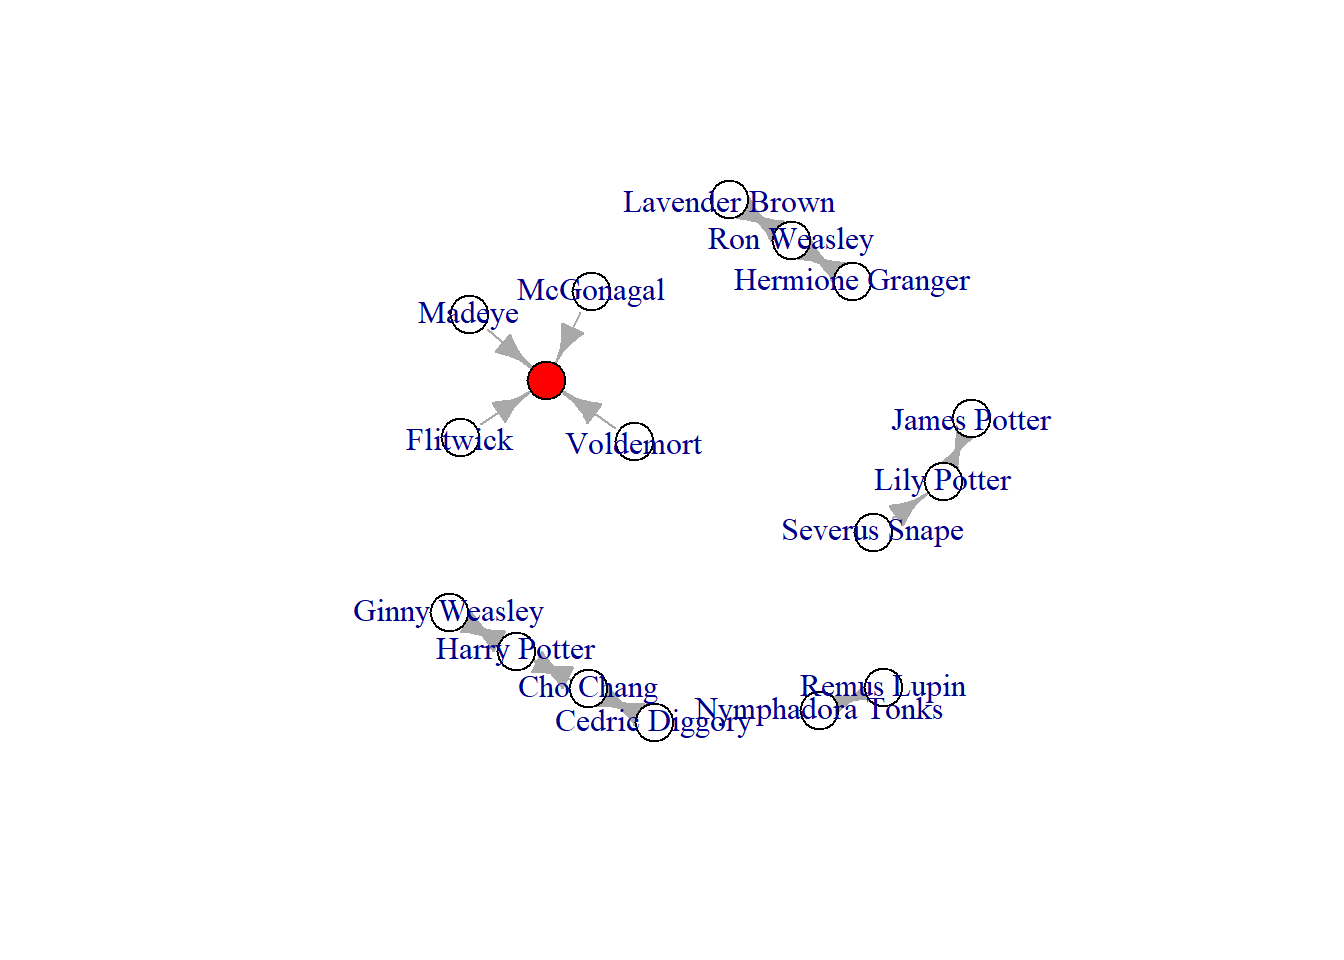
\includegraphics[keepaspectratio]{Cleaning-Network-Data---Trimming-and-Adding_files/figure-pdf/unnamed-chunk-6-2.pdf}}

One way to deal with this is to delete the superfluous node. You do this
using the delete\_vertex() function. \#\#This fixes the issue once you
have the data in Rstudio, but the issue still exists in your dataset. If
you choose to structure your network data this way, you will have to
remember to remove this node every time. This may be harder to
do/realise when dealing with large dense networks.

\begin{Shaded}
\begin{Highlighting}[]
\NormalTok{crush\_empty }\OtherTok{\textless{}{-}} \FunctionTok{delete\_vertices}\NormalTok{(crush\_empty, }\StringTok{""}\NormalTok{)}

\FunctionTok{plot}\NormalTok{(crush\_empty)}
\end{Highlighting}
\end{Shaded}

\pandocbounded{\includegraphics[keepaspectratio]{Cleaning-Network-Data---Trimming-and-Adding_files/figure-pdf/unnamed-chunk-7-1.pdf}}

Sometimes, you want to remove all of the isolated nodes from your
network because you only care about those who have connections to
others. To do this, you identify those with no connections (degree = 0)
and them remove them from your network. I suggest making a new object
with this sub network.

\begin{Shaded}
\begin{Highlighting}[]
\NormalTok{hog\_crush\_isol }\OtherTok{\textless{}{-}} \FunctionTok{which}\NormalTok{(}\FunctionTok{degree}\NormalTok{(crush\_empty)}\SpecialCharTok{==}\DecValTok{0}\NormalTok{)}
\end{Highlighting}
\end{Shaded}

Now you use the delete\_vertices() command and remove those in the
vector you just created (those with degree = 0)

\begin{Shaded}
\begin{Highlighting}[]
\NormalTok{Crush\_no\_isol }\OtherTok{\textless{}{-}}\FunctionTok{delete\_vertices}\NormalTok{(crush\_empty, hog\_crush\_isol)}

\FunctionTok{plot}\NormalTok{(Crush\_no\_isol)}
\end{Highlighting}
\end{Shaded}

\pandocbounded{\includegraphics[keepaspectratio]{Cleaning-Network-Data---Trimming-and-Adding_files/figure-pdf/unnamed-chunk-9-1.pdf}}

Now this new object has only those nodes with ties to others in the
network.

Other than isolates, you you might decide to remove one or more specific
nodes from your network. For example, in this hogwarts dataset, we may
want to remove those who are not students at Hogwarts (i.e.~remove
teachers or adults). To do this, you would use the delete\_vertices()
option.

Another approach is to delete them one-by-one and identify them by their
name. Let's say you have a network and only want to remove one node. You
can do so based on their name. To do this, let's now switch to the other
data we brought in, the one with the self loops (we will deal with those
next!). We can use the same function, delete\_vertices(), but this time,
state the name of the node we want to delete.

\begin{Shaded}
\begin{Highlighting}[]
\NormalTok{hog\_crush\_students }\OtherTok{\textless{}{-}} \FunctionTok{delete\_vertices}\NormalTok{(Crush\_loops, }\StringTok{"Voldemort"}\NormalTok{)}

\FunctionTok{plot}\NormalTok{(hog\_crush\_students)}
\end{Highlighting}
\end{Shaded}

\pandocbounded{\includegraphics[keepaspectratio]{Cleaning-Network-Data---Trimming-and-Adding_files/figure-pdf/unnamed-chunk-10-1.pdf}}

A quicker way, if you are deleting multiple, is to make a vector with
all the names of those you want to remove, then use the
delete\_vertices() command.

\begin{Shaded}
\begin{Highlighting}[]
\NormalTok{hog\_adults }\OtherTok{\textless{}{-}} \FunctionTok{c}\NormalTok{(}\StringTok{"Severus Snape"}\NormalTok{, }\StringTok{"Lily Potter"}\NormalTok{, }\StringTok{"James Potter"}\NormalTok{, }\StringTok{"Nymphadora Tonks"}\NormalTok{, }\StringTok{"Remus Lupin"}\NormalTok{, }\StringTok{"Voldemort"}\NormalTok{, }\StringTok{"Flitwick"}\NormalTok{, }\StringTok{"McGonagal"}\NormalTok{, }\StringTok{"Madeye"}\NormalTok{)}

\NormalTok{hog\_crush\_students }\OtherTok{\textless{}{-}} \FunctionTok{delete\_vertices}\NormalTok{(Crush\_loops, hog\_adults)}

\FunctionTok{plot}\NormalTok{(hog\_crush\_students)}
\end{Highlighting}
\end{Shaded}

\pandocbounded{\includegraphics[keepaspectratio]{Cleaning-Network-Data---Trimming-and-Adding_files/figure-pdf/unnamed-chunk-11-1.pdf}}

This new version removed all unwanted nodes at once.

\section{Deleting edges}\label{deleting-edges}

To remove unwanted edges you can use the delete\_edges() command. Let's
begin with our edgelist from above and select the edges that are looped
by using the E() command coupled with the is.loop() options.

\begin{Shaded}
\begin{Highlighting}[]
\NormalTok{Crush\_loops  }\OtherTok{\textless{}{-}} \FunctionTok{delete\_edges}\NormalTok{(Crush\_loops, }\FunctionTok{E}\NormalTok{(Crush\_loops )[}\FunctionTok{which\_loop}\NormalTok{(Crush\_loops)])}

\FunctionTok{plot}\NormalTok{(Crush\_loops)}
\end{Highlighting}
\end{Shaded}

\pandocbounded{\includegraphics[keepaspectratio]{Cleaning-Network-Data---Trimming-and-Adding_files/figure-pdf/unnamed-chunk-12-1.pdf}}

In addition to the selfloops, you may want to delete edges between two
specific nodes. You can do so by selecting

\begin{Shaded}
\begin{Highlighting}[]
\NormalTok{edges\_to\_delete }\OtherTok{\textless{}{-}} \FunctionTok{E}\NormalTok{(Crush\_loops)[(}\FunctionTok{.from}\NormalTok{(}\StringTok{"Remus Lupin"}\NormalTok{) }\SpecialCharTok{\&} \FunctionTok{.to}\NormalTok{(}\StringTok{"Nymphadora Tonks"}\NormalTok{))]}

\NormalTok{Crush\_edge\_delete }\OtherTok{\textless{}{-}} \FunctionTok{delete\_edges}\NormalTok{(Crush\_loops, edges\_to\_delete)}

\FunctionTok{plot}\NormalTok{(Crush\_edge\_delete)}
\end{Highlighting}
\end{Shaded}

\pandocbounded{\includegraphics[keepaspectratio]{Cleaning-Network-Data---Trimming-and-Adding_files/figure-pdf/unnamed-chunk-13-1.pdf}}

To delete all edges between two nodes.

\begin{Shaded}
\begin{Highlighting}[]
\NormalTok{edges\_to\_delete2 }\OtherTok{\textless{}{-}} \FunctionTok{E}\NormalTok{(Crush\_loops)[(}\FunctionTok{.from}\NormalTok{(}\StringTok{"Remus Lupin"}\NormalTok{) }\SpecialCharTok{\&} \FunctionTok{.to}\NormalTok{(}\StringTok{"Nymphadora Tonks"}\NormalTok{)) }\SpecialCharTok{|} \FunctionTok{.from}\NormalTok{(}\StringTok{"Nymphadora Tonks"}\NormalTok{) }\SpecialCharTok{\&} \FunctionTok{.to}\NormalTok{(}\StringTok{"Remus Lupin"}\NormalTok{)]}

\NormalTok{Crush\_edge\_delete }\OtherTok{\textless{}{-}} \FunctionTok{delete\_edges}\NormalTok{(Crush\_loops, edges\_to\_delete2)}

\FunctionTok{plot}\NormalTok{(Crush\_edge\_delete)}
\end{Highlighting}
\end{Shaded}

\pandocbounded{\includegraphics[keepaspectratio]{Cleaning-Network-Data---Trimming-and-Adding_files/figure-pdf/unnamed-chunk-14-1.pdf}}

\section{Adding Nodes}\label{adding-nodes}

Next, you might need to add data to the network object. Use caution when
doing this. Consider the ethics of your research. Has the person you are
adding consented to being studied? Adding data, any data, requires
consideration.

Once you have considered the above and are sure that it is ethical to
add data to your network, you may wish to add nodes to your network. To
do so, use add.vertices() function.

\begin{Shaded}
\begin{Highlighting}[]
\NormalTok{crush\_added }\OtherTok{\textless{}{-}} \FunctionTok{add.vertices}\NormalTok{(Crush\_loops, }\DecValTok{1}\NormalTok{, }\AttributeTok{name =} \StringTok{"Michael Corner"}\NormalTok{)  }

\FunctionTok{plot}\NormalTok{(crush\_added)}
\end{Highlighting}
\end{Shaded}

\pandocbounded{\includegraphics[keepaspectratio]{Cleaning-Network-Data---Trimming-and-Adding_files/figure-pdf/unnamed-chunk-15-1.pdf}}

This function follows the following logic: you state the network that
you want to add to, state how many nodes you are adding (in this case
1), then state the attribute of the node you are adding (in this case,
the name is ``Michael Corner.''

\section{Add Edges}\label{add-edges}

You may need to add edges that you know exist. For example, in this
network, the node that we added, ``Michael Corner'' has connections to
another in this network! So, when I originally collected these network
data, I forgot this guy! Note, these are fictional people, so I do not
need to check with ``Michael Corner'' before I add him and his
connections to our network.

We have added him in, but now we need to add his connections. To do
this, you use add.edges().Note, that we start with Michael, then we list
to whom he is connected. Think of this as a ``from'' and ``to'' formula.
So here, this goes from ``Michael Corner'' to ``Ginny Weasley.''

\begin{Shaded}
\begin{Highlighting}[]
\NormalTok{crush\_added }\OtherTok{\textless{}{-}} \FunctionTok{add.edges}\NormalTok{(crush\_added, }\AttributeTok{edges =} \FunctionTok{c}\NormalTok{(}\StringTok{"Michael Corner"}\NormalTok{, }\StringTok{"Ginny Weasley"}\NormalTok{))}

\FunctionTok{plot}\NormalTok{(crush\_added)}
\end{Highlighting}
\end{Shaded}

\pandocbounded{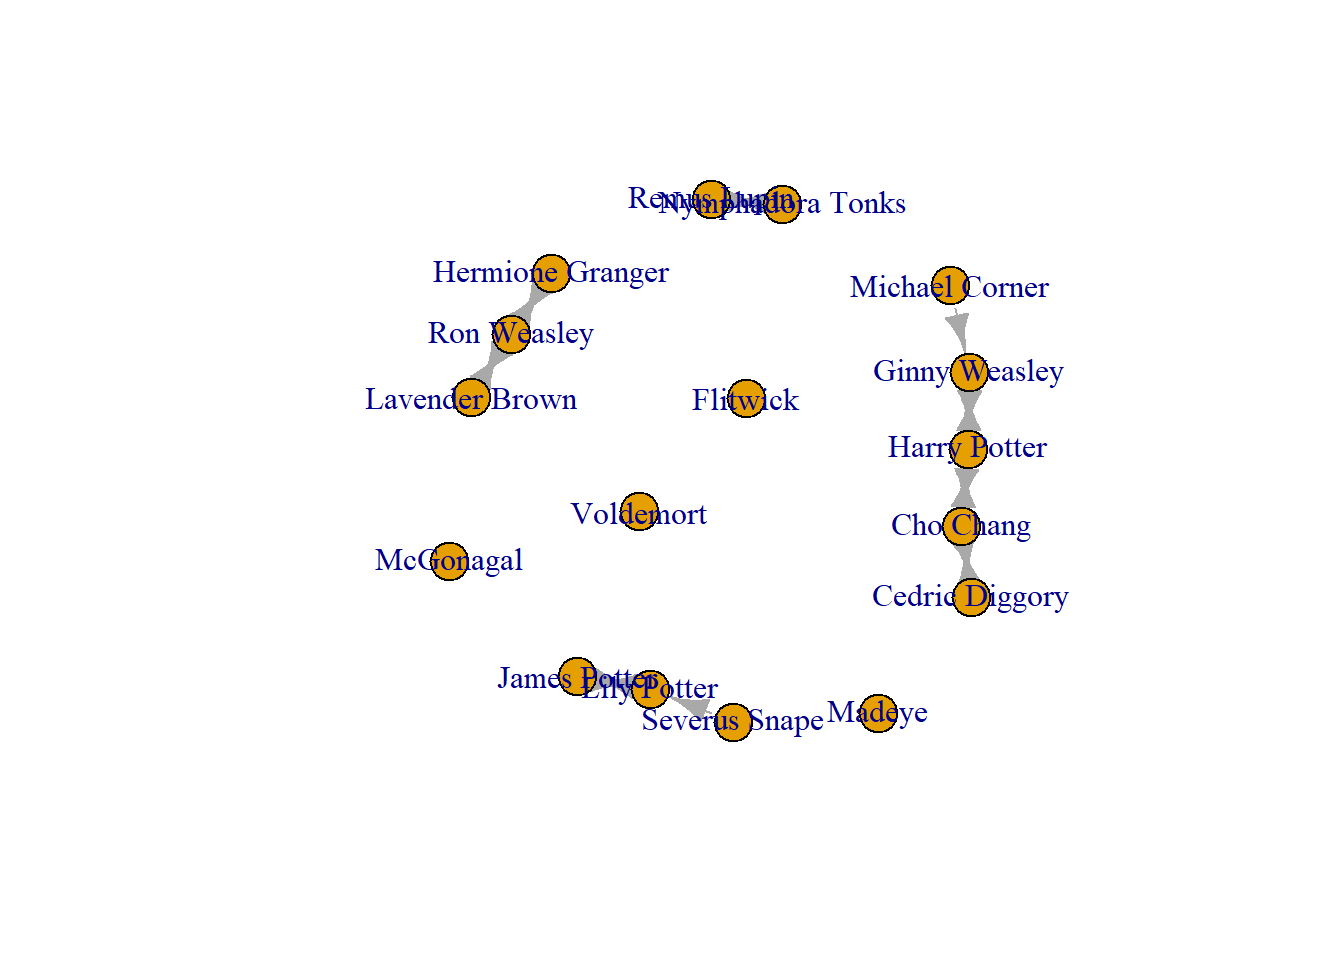
\includegraphics[keepaspectratio]{Cleaning-Network-Data---Trimming-and-Adding_files/figure-pdf/unnamed-chunk-16-1.pdf}}

Now to add the reciprocated tie, from ``Gunny Wealey'' to ``Michael
Corner.''

\begin{Shaded}
\begin{Highlighting}[]
\NormalTok{crush\_added }\OtherTok{\textless{}{-}} \FunctionTok{add.edges}\NormalTok{(crush\_added, }\AttributeTok{edges =} \FunctionTok{c}\NormalTok{(}\StringTok{"Ginny Weasley"}\NormalTok{, }\StringTok{"Michael Corner"}\NormalTok{))}
                         
\FunctionTok{plot}\NormalTok{(crush\_added)}
\end{Highlighting}
\end{Shaded}

\pandocbounded{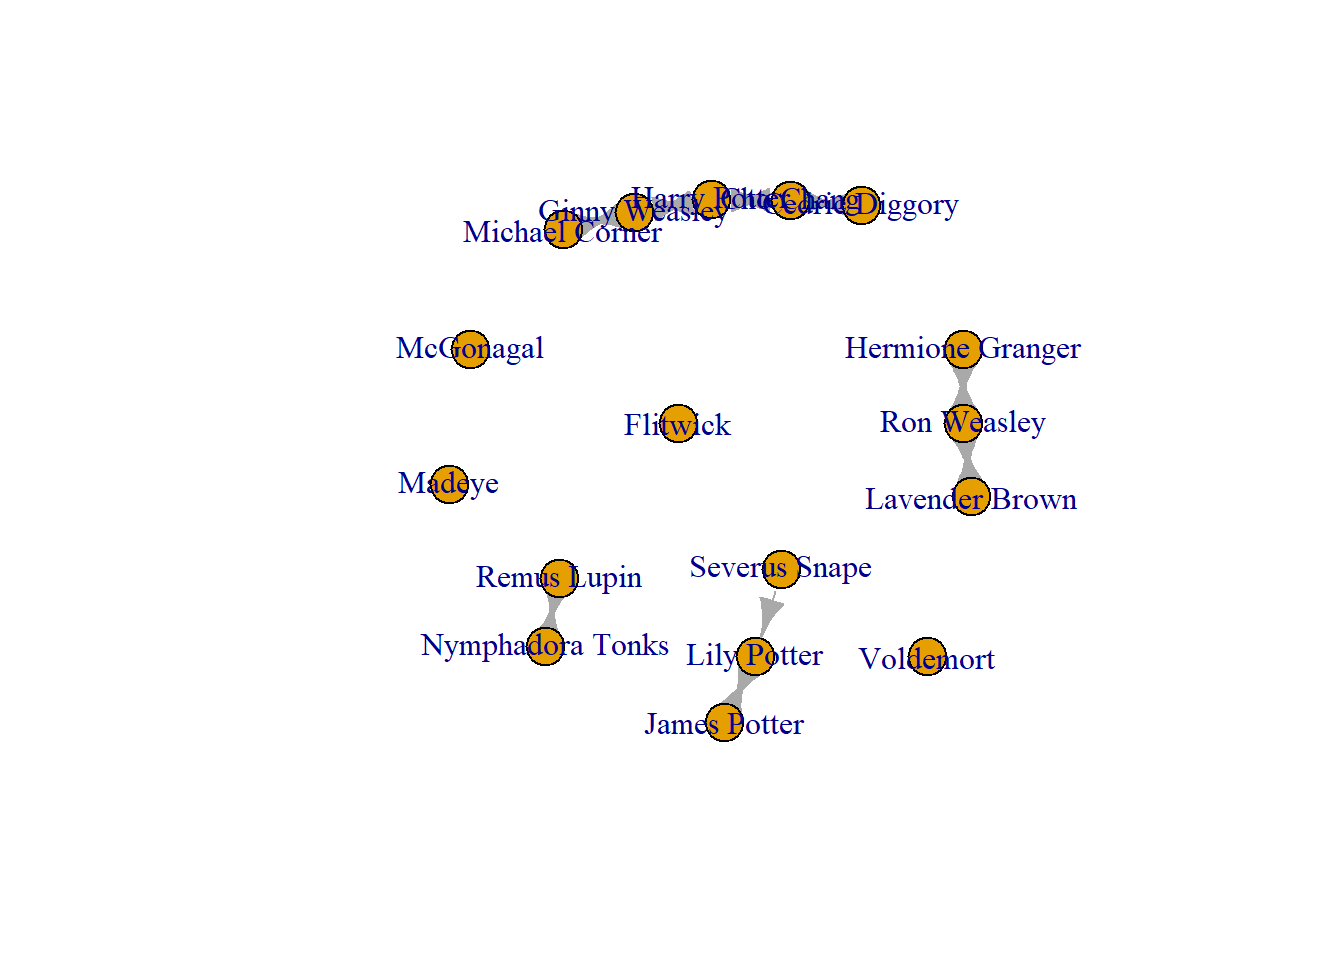
\includegraphics[keepaspectratio]{Cleaning-Network-Data---Trimming-and-Adding_files/figure-pdf/unnamed-chunk-17-1.pdf}}

\section{Summary}\label{summary-1}

Here we have covered a few ways to clean network data. We have covered a
few tings.

\begin{enumerate}
\def\labelenumi{\arabic{enumi}.}
\item
  Network data can be messy
\item
  Adding or delete nodes and edges either systematically (i.e.~all
  isolates) or one-by-one.
\end{enumerate}

Well done!

\chapter{Cleaning Network Data -
Subgraphs}\label{cleaning-network-data---subgraphs}

\begin{Shaded}
\begin{Highlighting}[]
\FunctionTok{library}\NormalTok{(igraph)}
\FunctionTok{library}\NormalTok{(ADAPTSNA)}
\end{Highlighting}
\end{Shaded}

You may want to create subgraphs of the network that you have. There are
two basic ways that you can think about this. You may be interested in a
specific group of people and how they relate to each other, or you may
be interested in a specific person and find out who they are connected
to.

\begin{longtable}[]{@{}
  >{\raggedright\arraybackslash}p{(\linewidth - 0\tabcolsep) * \real{1.0067}}@{}}
\toprule\noalign{}
\begin{minipage}[b]{\linewidth}\raggedright
\textbf{LEARNING ELEMENTS - Data Discoveries}
\end{minipage} \\
\midrule\noalign{}
\endhead
\bottomrule\noalign{}
\endlastfoot
\begin{minipage}[t]{\linewidth}\raggedright
\begin{itemize}
\item
  There are levels of network analysis. Sociocentric networks are the
  whole group while egocentric networks are the network of an
  individual.
\item
  You might have sociocentric network data and discover an interesting
  story about an individual or a smaller group. For this, you need
  subgraphs.
\end{itemize}
\end{minipage} \\
\end{longtable}

First, we start by bringing in the data and cleaning out the self loops.
This new dataset is of some Grime musicians from Spotify. The nodes are
the artists and the ties represent collaborations between the artists.

\begin{Shaded}
\begin{Highlighting}[]
\NormalTok{grime\_edge\_list }\OtherTok{\textless{}{-}} \FunctionTok{load\_data}\NormalTok{(}\StringTok{"GRIME\_2008\_Edge.csv"}\NormalTok{, }\AttributeTok{header =} \ConstantTok{TRUE}\NormalTok{)}

\NormalTok{grime\_08 }\OtherTok{\textless{}{-}} \FunctionTok{graph\_from\_data\_frame}\NormalTok{(}\AttributeTok{d=}\NormalTok{ grime\_edge\_list, }\AttributeTok{directed =} \ConstantTok{TRUE}\NormalTok{)}
\end{Highlighting}
\end{Shaded}

\begin{Shaded}
\begin{Highlighting}[]
\NormalTok{grime\_08\_clean }\OtherTok{\textless{}{-}} \FunctionTok{delete\_edges}\NormalTok{(grime\_08, }\FunctionTok{E}\NormalTok{(grime\_08)[}\FunctionTok{which\_loop}\NormalTok{(grime\_08)])}
\end{Highlighting}
\end{Shaded}

\section{Specific Subgraphs}\label{specific-subgraphs}

First, let's talk asume you need a subgraph to see a specific set of
people and how/whether they are connected. You may have a list of
individual nodes that you are interested in and you want to see how they
related to each other. You can do this by creating a vector with the
names of those nodes, then use the subgraph function().

Why might you want to do this? There could be a highly prominent
individual, or group of individuals in the network and you might want to
see how these individuals are connected.~Here, the individuals, Wiley,
Jammer, Flowdan, and Ice Kid, are some of the older generation grime
artists. In this network, taken from 2008, it might be interesting to
see how/if these individuals are connected.

\begin{Shaded}
\begin{Highlighting}[]
\NormalTok{sub\_people }\OtherTok{\textless{}{-}} \FunctionTok{c}\NormalTok{(}\StringTok{\textquotesingle{}Wiley\textquotesingle{}}\NormalTok{, }\StringTok{\textquotesingle{}Jammer\textquotesingle{}}\NormalTok{, }\StringTok{\textquotesingle{}Flowdan\textquotesingle{}}\NormalTok{, }\StringTok{\textquotesingle{}Ice Kid\textquotesingle{}}\NormalTok{)}
\NormalTok{sub\_net }\OtherTok{\textless{}{-}} \FunctionTok{subgraph}\NormalTok{(grime\_08\_clean, sub\_people) }
\FunctionTok{par}\NormalTok{(}\AttributeTok{mar =} \FunctionTok{c}\NormalTok{(}\DecValTok{0}\NormalTok{,}\DecValTok{0}\NormalTok{,}\DecValTok{0}\NormalTok{,}\DecValTok{0}\NormalTok{))}
\FunctionTok{plot}\NormalTok{(sub\_net)}
\end{Highlighting}
\end{Shaded}

\pandocbounded{\includegraphics[keepaspectratio]{Cleaning-Network-Data---Subgraphs_files/figure-pdf/unnamed-chunk-4-1.pdf}}

\section{Ego Graphs}\label{ego-graphs}

Next, you may want to see ego networks from those in your network. In
other words, smaller networks showing only the connections of each
individual artist. To do this, you can use the make\_ego\_graph()
argument. This creates a list of ego graphs from your entire network.
Note, the order = 1 argument refers to the number of steps away from the
ego (focal node). Since mine is set to 1, this only captures the ego's
immediate neighbours (i.e.~only those directly connected to ego).

\begin{Shaded}
\begin{Highlighting}[]
\NormalTok{ego\_graphs }\OtherTok{\textless{}{-}} \FunctionTok{make\_ego\_graph}\NormalTok{(grime\_08\_clean, }\AttributeTok{order =} \DecValTok{1}\NormalTok{)}
\FunctionTok{head}\NormalTok{(ego\_graphs)}
\end{Highlighting}
\end{Shaded}

\begin{verbatim}
[[1]]
IGRAPH 74caf2e DN-- 2 1 -- 
+ attr: name (v/c), collab_weight (e/n)
+ edge from 74caf2e (vertex names):
[1] Asher D->Wiley

[[2]]
IGRAPH 74caf54 DN-- 1 0 -- 
+ attr: name (v/c), collab_weight (e/n)
+ edges from 74caf54 (vertex names):

[[3]]
IGRAPH 74caf66 DN-- 1 0 -- 
+ attr: name (v/c), collab_weight (e/n)
+ edges from 74caf66 (vertex names):

[[4]]
IGRAPH 74caf76 DN-- 2 1 -- 
+ attr: name (v/c), collab_weight (e/n)
+ edge from 74caf76 (vertex names):
[1] Scorcher->Wiley

[[5]]
IGRAPH 74caf87 DN-- 3 2 -- 
+ attr: name (v/c), collab_weight (e/n)
+ edges from 74caf87 (vertex names):
[1] Bless Beats->Wiley     Bless Beats->Roll Deep

[[6]]
IGRAPH 74caf97 DN-- 3 2 -- 
+ attr: name (v/c), collab_weight (e/n)
+ edges from 74caf97 (vertex names):
[1] Flowdan->Wiley  Flowdan->Jammer
\end{verbatim}

You can also specify exactly which node's network you want to see. Let's
say there was a person of interest in your network that you specifically
want to see. To do this, you can do the following using the node's name
to single them out.

This chunk returns a list of edges connected to Wiley (the name of my
node of interest).

\begin{Shaded}
\begin{Highlighting}[]
\FunctionTok{E}\NormalTok{(grime\_08\_clean)[[}\FunctionTok{.inc}\NormalTok{(}\StringTok{\textquotesingle{}Wiley\textquotesingle{}}\NormalTok{)]]}
\end{Highlighting}
\end{Shaded}

\begin{verbatim}
+ 8/28 edges from 74c262e (vertex names):
             tail         head tid hid collab_weight
1         Asher D        Wiley   1  29             1
2        Scorcher        Wiley   4  29             4
3     Bless Beats        Wiley   5  29             1
4         Flowdan        Wiley   6  29             3
5  Tinchy Stryder        Wiley   7  29             2
6          Frisco        Wiley   8  29             1
7            Kano        Wiley   9  29             1
27          Wiley Lauren Mason  29  39             1
\end{verbatim}

I can also plot these. To do so, I make an object with the name `Wiley'
and then make an ego graph based on that name only. The {[}{[}1{]}{]}
simply tells R to get only the first one in the list that
make\_ego\_graph() creates. In this case, Wiley. Using the ``order = 1''
option, you are selecting to gather Wiley's immediate neighbours (known
as a first order ego network).

\begin{Shaded}
\begin{Highlighting}[]
\NormalTok{Wiley }\OtherTok{\textless{}{-}} \StringTok{"Wiley"}
\NormalTok{ego\_wiley }\OtherTok{\textless{}{-}} \FunctionTok{make\_ego\_graph}\NormalTok{(grime\_08\_clean, }\AttributeTok{order =} \DecValTok{1}\NormalTok{, }\AttributeTok{nodes =}\NormalTok{ Wiley)[[}\DecValTok{1}\NormalTok{]]}

\FunctionTok{par}\NormalTok{(}\AttributeTok{mar =} \FunctionTok{c}\NormalTok{(}\DecValTok{0}\NormalTok{,}\DecValTok{0}\NormalTok{,}\DecValTok{0}\NormalTok{,}\DecValTok{0}\NormalTok{))}
\FunctionTok{plot}\NormalTok{(ego\_wiley)}
\end{Highlighting}
\end{Shaded}

\pandocbounded{\includegraphics[keepaspectratio]{Cleaning-Network-Data---Subgraphs_files/figure-pdf/unnamed-chunk-7-1.pdf}}

The second order ego network includes the connections of Wiley's
neighbours. This is useful to see whether/how Wiley's connections are
also collaborating.

\begin{Shaded}
\begin{Highlighting}[]
\NormalTok{second\_order\_wiley }\OtherTok{\textless{}{-}} \FunctionTok{make\_ego\_graph}\NormalTok{(grime\_08\_clean, }\AttributeTok{order =} \DecValTok{2}\NormalTok{, }\AttributeTok{nodes =}\NormalTok{ Wiley)[[}\DecValTok{1}\NormalTok{]]}

\FunctionTok{par}\NormalTok{(}\AttributeTok{mar =} \FunctionTok{c}\NormalTok{(}\DecValTok{0}\NormalTok{,}\DecValTok{0}\NormalTok{,}\DecValTok{0}\NormalTok{,}\DecValTok{0}\NormalTok{))}
\FunctionTok{plot}\NormalTok{(second\_order\_wiley)}
\end{Highlighting}
\end{Shaded}

\pandocbounded{\includegraphics[keepaspectratio]{Cleaning-Network-Data---Subgraphs_files/figure-pdf/unnamed-chunk-8-1.pdf}}

Pro tip: If you are working with ego networks like this, especially when
you get passed the first order network (including friends of friends) it
is good practice to do something to differentiate the ego from their
neighbours. This way, someone who is looking at the graph can clearly
identify who is the ego and who are the neighbours. One simple way it to
change their colour.

Don't get too caught up in this code below. We will cover a lot more of
this in future chapters (see
\href{Intermediate\%20Visualisation.qmd}{Chapter 11}. What we do here is
create a node characteristic called `ego'. What this characeristic does
is assign colours to every node in the network. If the name of that node
is ``Wiley'' then the colour is red, otherwise it is white. The next
chunk changes the parameters of the plot so we can see it a bit easier.
Then, using the vertex.color option of the plot() function, we change
the colour of the visualisation to reflect the red and white that we
just added.

\begin{Shaded}
\begin{Highlighting}[]
\FunctionTok{V}\NormalTok{(second\_order\_wiley)}\SpecialCharTok{$}\NormalTok{ego }\OtherTok{\textless{}{-}} \FunctionTok{ifelse}\NormalTok{(}\FunctionTok{V}\NormalTok{(second\_order\_wiley)}\SpecialCharTok{$}\NormalTok{name }\SpecialCharTok{\%in\%} \FunctionTok{c}\NormalTok{(}\StringTok{"Wiley"}\NormalTok{), }\StringTok{"red"}\NormalTok{, }\StringTok{"white"}\NormalTok{)}

\FunctionTok{par}\NormalTok{(}\AttributeTok{mar =} \FunctionTok{c}\NormalTok{(}\DecValTok{0}\NormalTok{,}\DecValTok{0}\NormalTok{,}\DecValTok{3}\NormalTok{,}\DecValTok{0}\NormalTok{))}
\FunctionTok{plot}\NormalTok{(second\_order\_wiley, }\AttributeTok{vertex.color =} \FunctionTok{V}\NormalTok{(second\_order\_wiley)}\SpecialCharTok{$}\NormalTok{ego, }\AttributeTok{main =} \StringTok{"Wiley\textquotesingle{}s Second Order Ego Network"}\NormalTok{)}
\end{Highlighting}
\end{Shaded}

\pandocbounded{\includegraphics[keepaspectratio]{Cleaning-Network-Data---Subgraphs_files/figure-pdf/unnamed-chunk-9-1.pdf}}

Finally, one other way to can subset a network is by a set parameter you
may have. For example, you may want to see a network of frequent
collaborators (more than 1 collab).

The following returns a vector with collaborators who work together more
than once.

\begin{Shaded}
\begin{Highlighting}[]
\NormalTok{frequent\_collabors }\OtherTok{\textless{}{-}} \FunctionTok{E}\NormalTok{(grime\_08\_clean)[[collab\_weight }\SpecialCharTok{\textgreater{}} \DecValTok{1}\NormalTok{]]}
\NormalTok{frequent\_collabors}
\end{Highlighting}
\end{Shaded}

\begin{verbatim}
+ 8/28 edges from 74c262e (vertex names):
             tail   head tid hid collab_weight
2        Scorcher  Wiley   4  29             4
4         Flowdan  Wiley   6  29             3
5  Tinchy Stryder  Wiley   7  29             2
8          Blacks Jammer  12  35             4
9         Badness Jammer  13  35             5
11        Tempa T Jammer  15  35             2
14         Skepta Jammer  17  35             5
16         Frisco Jammer   8  35             3
\end{verbatim}

You can then turn this vector of edges into a igraph object to plot.

\begin{Shaded}
\begin{Highlighting}[]
\NormalTok{frequent\_collabors\_graph }\OtherTok{\textless{}{-}} \FunctionTok{induced\_subgraph}\NormalTok{(grime\_08\_clean, }\AttributeTok{vids =} \FunctionTok{unique}\NormalTok{(}\FunctionTok{c}\NormalTok{(}\FunctionTok{ends}\NormalTok{(grime\_08\_clean, frequent\_collabors)[, }\DecValTok{1}\NormalTok{], }\FunctionTok{ends}\NormalTok{(grime\_08\_clean, frequent\_collabors)[, }\DecValTok{2}\NormalTok{])))}
\FunctionTok{plot}\NormalTok{(frequent\_collabors\_graph)}
\end{Highlighting}
\end{Shaded}

\pandocbounded{\includegraphics[keepaspectratio]{Cleaning-Network-Data---Subgraphs_files/figure-pdf/unnamed-chunk-11-1.pdf}}

\section{Summary}\label{summary-2}

Here we have discussed another method for cleaning network data, taking
a subgraph. This is a simple cleaning or transformation tool that allows
you to study a subset of your data. We have covered how to take a
specific subset based on the names of particular nodes of interest.
Alternatively, we can we can create ego networks.

\chapter{Node and Edge Attributes}\label{node-and-edge-attributes}

\begin{Shaded}
\begin{Highlighting}[]
\FunctionTok{library}\NormalTok{(igraph)}
\FunctionTok{library}\NormalTok{(ADAPTSNA)}
\end{Highlighting}
\end{Shaded}

Your network may have some edge characteristics. What this means is that
the network has qualitative or quantitative information regarding the
connections between nodes. These could be things that denote a certain
type of connection between individuals in the network (romantic
vs.~friend, positive vs.~negative, kinship vs.~friend). These
qualitatively different categories tell us more about the types of
relationships that there are between the nodes in our network.
Meanwhile, quantitative information can also tells us more about the
information. Quantitative information could include things like
frequency of communication. Such information is termed the edges
``weight'' indicating that there are substantively meaningful
differences between the levels of connection (for example interacting
only once compared to 10 times).

Additionally, your network may have some information about the nodes.
Such information could include categorical information (e.g demographics
or other categories) or numeric information (e.g.~age). This means we
can inform our visualisation to portray the information about the nodes.

All of this information can be attached to our edgelist. You can also do
this on an adjacency matrix but it is not as straightforward. To learn
the process, let's stick with edgelists.

\begin{longtable}[]{@{}
  >{\raggedright\arraybackslash}p{(\linewidth - 0\tabcolsep) * \real{1.0047}}@{}}
\toprule\noalign{}
\begin{minipage}[b]{\linewidth}\raggedright
LEARNING ELEMENTS - Data Perspectives and Practices
\end{minipage} \\
\midrule\noalign{}
\endhead
\bottomrule\noalign{}
\endlastfoot
\begin{minipage}[t]{\linewidth}\raggedright
\begin{itemize}
\item
  Network data can have missingness. If the node and edge
  characteristics are important to your study, then you may consider
  trimming your network to include only those who you have that
  information for.
\item
  Putting together pieces of network data. Recognise that the network
  itself can include data beyond just the existence of a tie. This
  section covers how to create a network object that has all available
  data.
\end{itemize}
\end{minipage} \\
\end{longtable}

\section{Getting to know these data}\label{getting-to-know-these-data}

This dataset has a lot more information about these individuals and
their relationships than others we have used this far. We have two excel
spreadsheets (.csv) one called vertices and the other called edges. The
vertices sheet has information about each individual node in the network
while the edges contains both the edges that exist as well as
information about them. Let's read them in and take a look at them

\begin{Shaded}
\begin{Highlighting}[]
\NormalTok{vertices.df }\OtherTok{\textless{}{-}} \FunctionTok{load\_data}\NormalTok{(}\StringTok{"Node data.csv"}\NormalTok{)}
\NormalTok{edges.df }\OtherTok{\textless{}{-}} \FunctionTok{load\_data}\NormalTok{(}\StringTok{"Edge data.csv"}\NormalTok{)}
\end{Highlighting}
\end{Shaded}

Let's take a look at these one at a tine to get an idea of what
information we have.

\begin{Shaded}
\begin{Highlighting}[]
\FunctionTok{head}\NormalTok{(edges.df)}
\end{Highlighting}
\end{Shaded}

\begin{verbatim}
  from to freq affinity
1    A  B    2      pos
2    A  C    1      neg
3    A  D    1      pos
4    A  E    1      neg
5    A  F    3      neg
6    E  F    2      pos
\end{verbatim}

We have an edgelist between A-F people. In this edgelist we have the
frequency of interaction and the affinity (i.e.~if they are positive or
negative interactions).

\begin{Shaded}
\begin{Highlighting}[]
\FunctionTok{head}\NormalTok{(vertices.df)}
\end{Highlighting}
\end{Shaded}

\begin{verbatim}
  name age role gender
1    A  20   DJ      F
2    B  25   MC      M
3    C  21   DJ      F
4    D  23 crew      M
5    E  24   MC      M
6    F  23   MC      F
\end{verbatim}

We have their name, age and two categorical variables about them, their
role (if they are a DJ or something else) and their sex (Male/Female).

Now I can create a network object in igraph using the familiar method
you are used to - graph\_from\_data\_frame(). However, We want this
network to have all the information possible. For this, we don't just
want the edge information, but also the node level information. To do
this, we tell R that the data = the edgelist.df (a familiar step to you
pros now!), and the vertex characteristics are stored in the object we
created earlier, vertices.df. Think of this step as simply pulling
information from your edgelist (E) and your vertices dataset (V) into
your network object.

\begin{Shaded}
\begin{Highlighting}[]
\NormalTok{graph }\OtherTok{\textless{}{-}} \FunctionTok{graph\_from\_data\_frame}\NormalTok{(}\AttributeTok{d =}\NormalTok{ edges.df, }\AttributeTok{vertices =}\NormalTok{ vertices.df , }\AttributeTok{directed =} \ConstantTok{FALSE}\NormalTok{)}

\NormalTok{graph}
\end{Highlighting}
\end{Shaded}

\begin{verbatim}
IGRAPH 7838e6b UN-- 7 7 -- 
+ attr: name (v/c), age (v/n), role (v/c), gender (v/c), freq (e/n),
| affinity (e/c)
+ edges from 7838e6b (vertex names):
[1] A--B A--C A--D A--E A--F E--F F--G
\end{verbatim}

Nice work! You can see the vertex information is stores as v
characteristics (name, age, role and gender. The edge characteristics
are stored as e characteristics - freq, affinity. Now lets visualise the
network and see what we have.

\begin{Shaded}
\begin{Highlighting}[]
\FunctionTok{plot}\NormalTok{(graph)}
\end{Highlighting}
\end{Shaded}

\pandocbounded{\includegraphics[keepaspectratio]{Node-and-Edge-Attributes_files/figure-pdf/unnamed-chunk-6-1.pdf}}

Here comes the fun part. First, let's start with the edge
characteristics. Rapid fire, we can visualise these in may different
ways.

\section{Exploring Edge
Characteristics}\label{exploring-edge-characteristics}

We will create a few visuals to demonstrate the information about these
edges. The main think you need to remember is that you access the edge
information of your network using the E() option.

Let's start with the numeric information we have about the edges. First,
we will change the width of the lines between nodes to reflect the
frequency of interactions using the edge.width argument and the freq
edge characteristic.

\begin{Shaded}
\begin{Highlighting}[]
\FunctionTok{plot}\NormalTok{(graph, }\AttributeTok{edge.width =} \FunctionTok{E}\NormalTok{(graph)}\SpecialCharTok{$}\NormalTok{freq)}
\end{Highlighting}
\end{Shaded}

\pandocbounded{\includegraphics[keepaspectratio]{Node-and-Edge-Attributes_files/figure-pdf/unnamed-chunk-7-1.pdf}}

Or, we can label the nodes with the frequency to tell a similar story.
We do this using the edge.label argument.

\begin{Shaded}
\begin{Highlighting}[]
\FunctionTok{plot}\NormalTok{(graph, }\AttributeTok{edge.label =} \FunctionTok{E}\NormalTok{(graph)}\SpecialCharTok{$}\NormalTok{freq)}
\end{Highlighting}
\end{Shaded}

\pandocbounded{\includegraphics[keepaspectratio]{Node-and-Edge-Attributes_files/figure-pdf/unnamed-chunk-8-1.pdf}}

What do these visuals tell you about their relationships compared to the
first one?

Now let's use the categorical information to tell a slightly different
story. Let's see what we can do to demonstrate the levels of affinity
between these individuals. First, we will change the line type to
reflect the different levels. To do this, we first create a logical
comparison using an ifelse statement. This checks if the affinity
attribute of each edge is equal to ``pos''. This will return a logical
vector (TRUE or FALSE for each edge). If the edge is ``pos'' then it
will return an item of the vector ``solid'' if it is false
(i.e.~``neg''), then it will return ``dotdash''. We can then visualise
this in the network using the edge.lty (lty means line type) argument.

\begin{Shaded}
\begin{Highlighting}[]
\CommentTok{\#change the line type using edge.lty to match the affinity}
\NormalTok{type\_affinity }\OtherTok{\textless{}{-}} \FunctionTok{ifelse}\NormalTok{(}\FunctionTok{E}\NormalTok{(graph)}\SpecialCharTok{$}\NormalTok{affinity }\SpecialCharTok{==} \StringTok{"pos"}\NormalTok{, }\StringTok{"solid"}\NormalTok{, }\StringTok{"dotdash"}\NormalTok{)}
\CommentTok{\# Plot plus colour}
\FunctionTok{plot}\NormalTok{(graph, }\AttributeTok{edge.lty =}\NormalTok{ type\_affinity)}
\end{Highlighting}
\end{Shaded}

\pandocbounded{\includegraphics[keepaspectratio]{Node-and-Edge-Attributes_files/figure-pdf/unnamed-chunk-9-1.pdf}}

Now, let's combine a few approaches. We will use the same ifelse
statement but will apply it to the colours of the edges. We will also
change the edge labels to reflect the affinity label alongside the line
type.

\begin{Shaded}
\begin{Highlighting}[]
\NormalTok{affinity }\OtherTok{\textless{}{-}} \FunctionTok{ifelse}\NormalTok{(}\FunctionTok{E}\NormalTok{(graph)}\SpecialCharTok{$}\NormalTok{affinity }\SpecialCharTok{==} \StringTok{"pos"}\NormalTok{, }\StringTok{"blue"}\NormalTok{, }\StringTok{"red"}\NormalTok{)}
\FunctionTok{plot}\NormalTok{(graph, }\AttributeTok{edge.color =}\NormalTok{ affinity, }\AttributeTok{edge.label =} \FunctionTok{E}\NormalTok{(graph)}\SpecialCharTok{$}\NormalTok{affinity, }\AttributeTok{edge.lty =}\NormalTok{ type\_affinity)}
\end{Highlighting}
\end{Shaded}

\pandocbounded{\includegraphics[keepaspectratio]{Node-and-Edge-Attributes_files/figure-pdf/unnamed-chunk-10-1.pdf}}

\section{Exploring Vertex Attributes}\label{exploring-vertex-attributes}

Now let's turn to the rest of our data and explore the network's vertex
attributes. Like before, you access the vertex information in your graph
object using the V() option.

We will start with the numerical characteristics of the attributes -
their age. First, let's change the labels to show their age.

\begin{Shaded}
\begin{Highlighting}[]
\FunctionTok{plot}\NormalTok{(graph, }\AttributeTok{vertex.label =} \FunctionTok{V}\NormalTok{(graph)}\SpecialCharTok{$}\NormalTok{age)}
\end{Highlighting}
\end{Shaded}

\pandocbounded{\includegraphics[keepaspectratio]{Node-and-Edge-Attributes_files/figure-pdf/unnamed-chunk-11-1.pdf}}

Now, let's change the colours based on certain parameters that we set
using an ifelse() statement.

\begin{Shaded}
\begin{Highlighting}[]
\NormalTok{over\_22 }\OtherTok{\textless{}{-}} \FunctionTok{ifelse}\NormalTok{(}\FunctionTok{V}\NormalTok{(graph)}\SpecialCharTok{$}\NormalTok{age }\SpecialCharTok{\textgreater{}} \DecValTok{22}\NormalTok{, }\StringTok{"red"}\NormalTok{, }\StringTok{"white"}\NormalTok{) }
\FunctionTok{plot}\NormalTok{(graph, }\AttributeTok{vertex.color =}\NormalTok{ over\_22, }\AttributeTok{veterx.label.color =} \StringTok{"Black"}\NormalTok{)}
\end{Highlighting}
\end{Shaded}

\pandocbounded{\includegraphics[keepaspectratio]{Node-and-Edge-Attributes_files/figure-pdf/unnamed-chunk-12-1.pdf}}

Next, let's work with the categorical variables. First we can change the
labels to show these, and then change the colours. See if you can follow
the following code chunks and think about what these new networks tell
us.

\begin{Shaded}
\begin{Highlighting}[]
\FunctionTok{plot}\NormalTok{(graph, }\AttributeTok{vertex.label =}\FunctionTok{V}\NormalTok{(graph)}\SpecialCharTok{$}\NormalTok{gender)}
\end{Highlighting}
\end{Shaded}

\pandocbounded{\includegraphics[keepaspectratio]{Node-and-Edge-Attributes_files/figure-pdf/unnamed-chunk-13-1.pdf}}

\begin{Shaded}
\begin{Highlighting}[]
\FunctionTok{plot}\NormalTok{(graph, }\AttributeTok{vertex.label =} \FunctionTok{V}\NormalTok{(graph)}\SpecialCharTok{$}\NormalTok{role)}
\end{Highlighting}
\end{Shaded}

\pandocbounded{\includegraphics[keepaspectratio]{Node-and-Edge-Attributes_files/figure-pdf/unnamed-chunk-14-1.pdf}}

\begin{Shaded}
\begin{Highlighting}[]
\NormalTok{gender }\OtherTok{\textless{}{-}} \FunctionTok{ifelse}\NormalTok{(}\FunctionTok{V}\NormalTok{(graph)}\SpecialCharTok{$}\NormalTok{gender }\SpecialCharTok{==} \StringTok{"M"}\NormalTok{, }\StringTok{"orange"}\NormalTok{, }\StringTok{"blue"}\NormalTok{)}
\FunctionTok{plot}\NormalTok{(graph, }\AttributeTok{vertex.color =}\NormalTok{ gender, }\AttributeTok{vertex.label.color =} \StringTok{"white"}\NormalTok{)}
\end{Highlighting}
\end{Shaded}

\pandocbounded{\includegraphics[keepaspectratio]{Node-and-Edge-Attributes_files/figure-pdf/unnamed-chunk-15-1.pdf}}

We have done a lot with ifelse statements here. This are great for
setting direct parameters or for working with dichotomous categories
(i.e.~the male/female one we have). However, we may want to create
colours for categories that have more than one and then visualise it. We
are going to use a different package, called dplyr to manipulate what we
have to create a vertex attribute that reflect colours based on a
categorical variable (their role).

\begin{Shaded}
\begin{Highlighting}[]
\FunctionTok{library}\NormalTok{(dplyr)}
\end{Highlighting}
\end{Shaded}

To do this, we will return to the original dataframe storing information
about the vertex characteristics. Then, we will use the mutate()
function to create a new variable that reflect a colour for each role.
See if you can follow the logic and look at what we end up with.

\begin{Shaded}
\begin{Highlighting}[]
\NormalTok{vertices.df }\OtherTok{\textless{}{-}}\NormalTok{ vertices.df }\SpecialCharTok{\%\textgreater{}\%}
  \FunctionTok{mutate}\NormalTok{(}\AttributeTok{role\_colour =} \FunctionTok{ifelse}\NormalTok{(role }\SpecialCharTok{==} \StringTok{"DJ"}\NormalTok{, }\StringTok{"blue"}\NormalTok{, role)) }
\NormalTok{vertices.df }\OtherTok{\textless{}{-}}\NormalTok{ vertices.df }\SpecialCharTok{\%\textgreater{}\%}
  \FunctionTok{mutate}\NormalTok{(}\AttributeTok{role\_colour =} \FunctionTok{ifelse}\NormalTok{(role }\SpecialCharTok{==} \StringTok{"MC"}\NormalTok{, }\StringTok{"orange"}\NormalTok{, role\_colour))}
\NormalTok{vertices.df }\OtherTok{\textless{}{-}}\NormalTok{ vertices.df }\SpecialCharTok{\%\textgreater{}\%}
  \FunctionTok{mutate}\NormalTok{(}\AttributeTok{role\_colour =} \FunctionTok{ifelse}\NormalTok{(role }\SpecialCharTok{==} \StringTok{"crew"}\NormalTok{, }\StringTok{"green"}\NormalTok{, role\_colour))}

\FunctionTok{head}\NormalTok{(vertices.df)}
\end{Highlighting}
\end{Shaded}

\begin{verbatim}
  name age role gender role_colour
1    A  20   DJ      F        blue
2    B  25   MC      M      orange
3    C  21   DJ      F        blue
4    D  23 crew      M       green
5    E  24   MC      M      orange
6    F  23   MC      F      orange
\end{verbatim}

Here is the breakdown of the above code, the mutate function creates a
new variable (what we call role\_colour). We then use an ifelse()
statement again to replace this new variable with the name of a colour
that matches each category that we have. So, the first line adds the
colour ``blue'' if role (our original categorical variable) is set to
``DJ''. If it is not, we replace it with the rest of the role variable.
You could just leave that blank, or NA and then those cells would
reflect that. So, if you were to run only that first line, you would see
a new column in your dataset with some cells saying blue while the rest
refelect the other categories. The next few lines of code repeat the
same logic, but there is a small difference. Instead of replacing the
new variable (role\_colour) with the old variable (role) if the logic in
the ifelse() statement if false as we did in the firs tline, we replace
it with the new variable. We do that because we want to keep the
replacements we have done already already.

Now, let's recreate our new network object following the above method.

\begin{Shaded}
\begin{Highlighting}[]
\NormalTok{graph }\OtherTok{\textless{}{-}} \FunctionTok{graph\_from\_data\_frame}\NormalTok{(}\AttributeTok{d =}\NormalTok{ edges.df, }\AttributeTok{vertices =}\NormalTok{ vertices.df , }\AttributeTok{directed =} \ConstantTok{FALSE}\NormalTok{)}

\NormalTok{graph}
\end{Highlighting}
\end{Shaded}

\begin{verbatim}
IGRAPH 787f995 UN-- 7 7 -- 
+ attr: name (v/c), age (v/n), role (v/c), gender (v/c), role_colour
| (v/c), freq (e/n), affinity (e/c)
+ edges from 787f995 (vertex names):
[1] A--B A--C A--D A--E A--F E--F F--G
\end{verbatim}

The network has the new v characteristic that we created - role\_colour.
Now we can visualise this network with the different colours for the
roles all represented on the visual.

\begin{Shaded}
\begin{Highlighting}[]
\FunctionTok{plot}\NormalTok{(graph, }\AttributeTok{vertex.color =} \FunctionTok{V}\NormalTok{(graph)}\SpecialCharTok{$}\NormalTok{role\_colour, }\AttributeTok{vertex.label.color =} \StringTok{"white"}\NormalTok{)}
\end{Highlighting}
\end{Shaded}

\pandocbounded{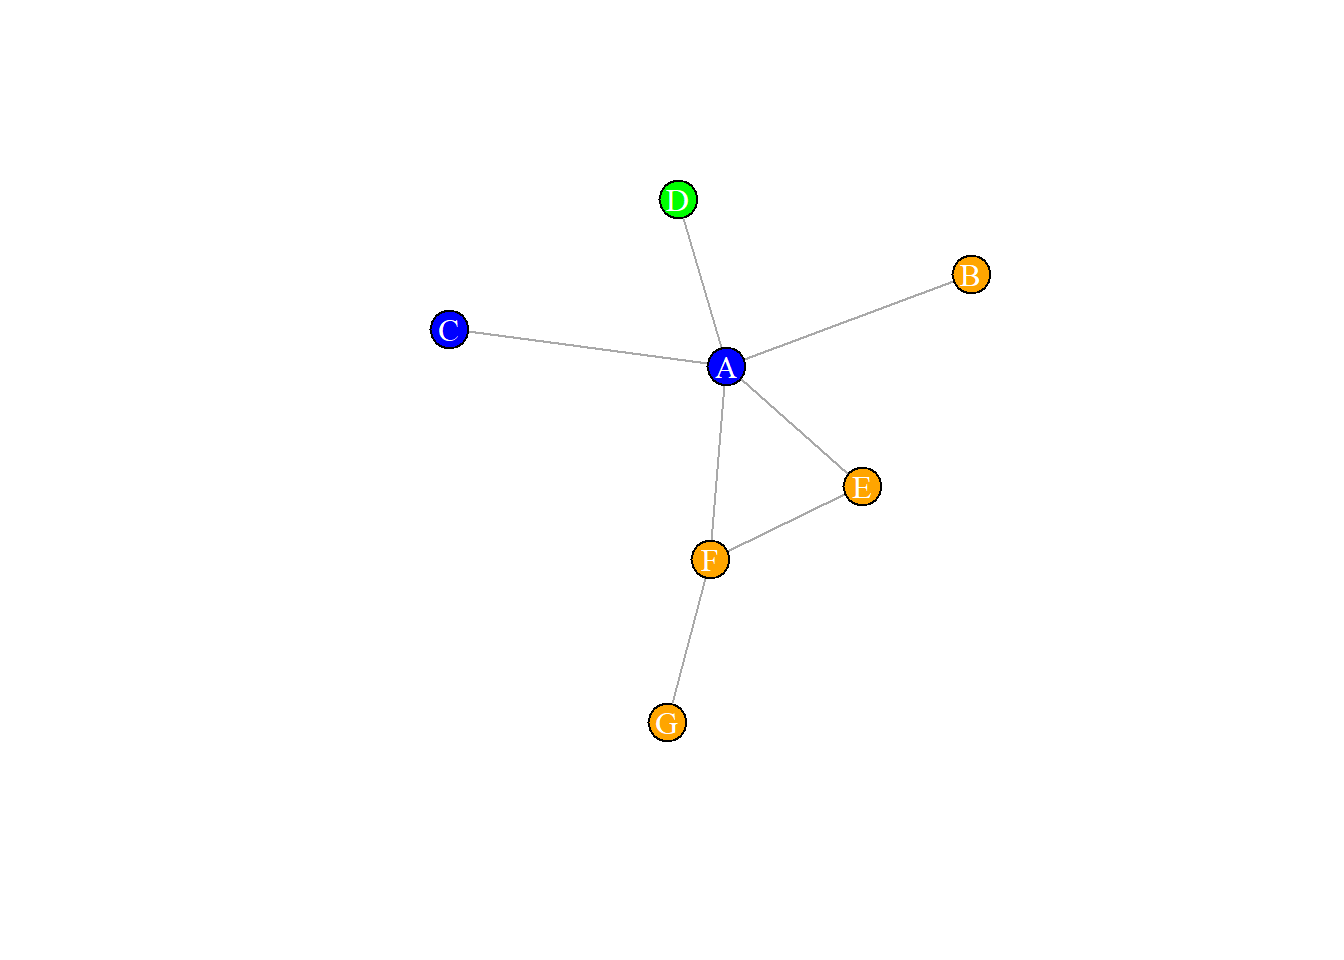
\includegraphics[keepaspectratio]{Node-and-Edge-Attributes_files/figure-pdf/unnamed-chunk-19-1.pdf}}

\section{Summary}\label{summary-3}

Your network data might have more information about the individuals and
their relationships. In this section, you have learned how to:

\begin{enumerate}
\def\labelenumi{\arabic{enumi}.}
\tightlist
\item
  Structure node and vertex attributes in data frames and bring them
  into R.
\item
  How to create a network object that contains the vertex and edge
  attributes.
\item
  How to transform the network data you have to generate visualisations
  portraying these node and edge attributes.
\end{enumerate}

GREAT WORK!

\chapter{Two Mode Networks - Adjacency
Matrix}\label{two-mode-networks---adjacency-matrix}

\begin{Shaded}
\begin{Highlighting}[]
\FunctionTok{library}\NormalTok{(igraph)}
\FunctionTok{library}\NormalTok{(ADAPTSNA)}
\end{Highlighting}
\end{Shaded}

Social network data can be one mode or two mode. So far we have dealt
with one mode network data. This means that one type of node is
connected to the same type of node. Individuals connected to other
individuals. We can also measure networks where there are two types of
node. Let's say individuals connected to groups that they participate
in.

\begin{longtable}[]{@{}
  >{\raggedright\arraybackslash}p{(\linewidth - 0\tabcolsep) * \real{1.0055}}@{}}
\toprule\noalign{}
\begin{minipage}[b]{\linewidth}\raggedright
LEARNING ELEMENTS - Data Practices
\end{minipage} \\
\midrule\noalign{}
\endhead
\bottomrule\noalign{}
\endlastfoot
\begin{minipage}[t]{\linewidth}\raggedright
\begin{itemize}
\item
  Data structure. Two mode networks can be structured in an adjacency
  matrix or an edgelist the same as one mode network data. The next two
  sections show how to bring them into R.
\item
  Communicating Two Mode Networks. This section provides some insight
  into effectively visualising two mode networks.
\end{itemize}
\end{minipage} \\
\end{longtable}

\section{Getting to Know the Data}\label{getting-to-know-the-data}

For this and the next chapter we will use some unique data where
individuals are connected to groups. Specifically, this dataset
demosntrates characters from the Harry Potter books auhtored by J.K.
Rowling who are connected to various groups across the serries.

I identified various groups from the series and then researched which
characters are participants in the groups. For example, I googled ``list
of prefects at hogwarts.'' Same for phoenix, death eaters etc. Most of
the info came from this site -
https://harrypotter.fandom.com/wiki/Dumbledore\%27s\_Army. I then
checked each person on google to see what house they were in - some are
missing and NA because they are fake characters from the movies or the
wiki page. I then structured these into an adjacency matrix and an
edgelist. In this chapter, we work on adjacecny matrices. We will deal
with the rest in the next chapter.

\begin{Shaded}
\begin{Highlighting}[]
\NormalTok{hp }\OtherTok{\textless{}{-}} \FunctionTok{load\_data}\NormalTok{(}\StringTok{"Harry Potter\_Two\_Mode\_AM.csv"}\NormalTok{, }\AttributeTok{row.names=}\DecValTok{1}\NormalTok{)}

\NormalTok{hp\_mat }\OtherTok{\textless{}{-}} \FunctionTok{as.matrix}\NormalTok{(hp)}

\FunctionTok{head}\NormalTok{(hp\_mat)}
\end{Highlighting}
\end{Shaded}

\begin{verbatim}
                 Phoenix Dumbeldore.s.Army Death.Eaters Inquisitorial.Squad
Albus Dumbledore       1                 0            0                   0
Remus Lupin            1                 0            0                   0
Molly Weasley          1                 0            0                   0
Siruis Black           1                 0            0                   0
Severus Snape          1                 0            1                   0
Alastor Moody          1                 0            0                   0
                 Prefect Gryffindor Ravenclaw Hufflepuff Slytherin
Albus Dumbledore       1          1         0          0         0
Remus Lupin            1          1         0          0         0
Molly Weasley          0          1         0          0         0
Siruis Black           0          1         0          0         0
Severus Snape          0          0         0          0         1
Alastor Moody          0          0         0          1         0
\end{verbatim}

\section{Two Mode Adjacency Matrices}\label{two-mode-adjacency-matrices}

So, here we have a two mode adjacency matrix. You will notice some
things that are similar to you, perhaps the 1/0 nature of a matrix. But
this is slightly different. The columns no longer reflect the same names
as the rows. Now, instead of an i,j matrix we have an i,g (group)
matrix. This means that there is no diagonal. Why? Well, because the
names at the top of the matrix (columns) are different from the side
(rows). Here then, i is sending to the group. Rather, we talk about
this, usually, in terms of affiliation. So, i is affiliated with the
group (or not).

For R to understand this is a two mode network matrix, we use a slightly
different command than a regular matrix.
graph\_from\_biadjacency\_matrix() is the current function where R
recognises the separate column names as one type of node and the row
names as another. For this to truly be a two mode network, they have to
be distinct.

\begin{Shaded}
\begin{Highlighting}[]
\NormalTok{hp\_aff }\OtherTok{\textless{}{-}} \FunctionTok{graph\_from\_biadjacency\_matrix}\NormalTok{(hp\_mat)}


\FunctionTok{plot}\NormalTok{(hp\_aff)}
\end{Highlighting}
\end{Shaded}

\pandocbounded{\includegraphics[keepaspectratio]{Two-Mode-Networks---AM_files/figure-pdf/unnamed-chunk-3-1.pdf}}

Looking at this plot, you can't tell if it is a one more or a two mode
network since the nodes all look exactly the same. There are a few
things we need to do in order to make this clearer.

\section{Visualising Two Mode
Networks}\label{visualising-two-mode-networks}

Let's make the visualisation much clearer between the two types of
nodes.

I do this by changing the shape and the colour of each type of node. I
set a vector with the colours and shapes I want

\begin{Shaded}
\begin{Highlighting}[]
\NormalTok{shapes }\OtherTok{\textless{}{-}} \FunctionTok{c}\NormalTok{(}\StringTok{"circle"}\NormalTok{, }\StringTok{"square"}\NormalTok{)}
\NormalTok{colors }\OtherTok{\textless{}{-}}\FunctionTok{c}\NormalTok{(}\StringTok{"green"}\NormalTok{, }\StringTok{"orange"}\NormalTok{)}
\end{Highlighting}
\end{Shaded}

Then we can plot them based on these design parameters

\begin{Shaded}
\begin{Highlighting}[]
\FunctionTok{par}\NormalTok{(}\AttributeTok{mar =}\FunctionTok{c}\NormalTok{(}\DecValTok{5}\NormalTok{,}\DecValTok{0}\NormalTok{,}\DecValTok{2}\NormalTok{,}\DecValTok{0}\NormalTok{))}
\FunctionTok{set.seed}\NormalTok{(}\DecValTok{123}\NormalTok{)}
\FunctionTok{plot}\NormalTok{(hp\_aff, }\AttributeTok{vertex.color=}\NormalTok{colors[}\FunctionTok{V}\NormalTok{(hp\_aff)}\SpecialCharTok{$}\NormalTok{type}\SpecialCharTok{+}\DecValTok{1}\NormalTok{],}
     \AttributeTok{vertex.shape=}\NormalTok{shapes[}\FunctionTok{V}\NormalTok{(hp\_aff)}\SpecialCharTok{$}\NormalTok{type}\SpecialCharTok{+}\DecValTok{1}\NormalTok{], }\AttributeTok{vertex.label.cex =} \FloatTok{0.5}\NormalTok{, }\AttributeTok{vertex.size =} \DecValTok{7}\NormalTok{, }\AttributeTok{main =} \StringTok{"Harry Potter"}\NormalTok{, }\AttributeTok{sub =} \StringTok{"Characters Connected to Groups"}\NormalTok{)}
\end{Highlighting}
\end{Shaded}

\pandocbounded{\includegraphics[keepaspectratio]{Two-Mode-Networks---AM_files/figure-pdf/unnamed-chunk-5-1.pdf}}

Here, I tell R to use the indices I've defined in the shapes and colors
vectors and apply those to the network using the vertex.shape and
vertex.color arguments. Notice that I need to state type + 1 in both of
these arguments. It might look a bit unusual at first, but it makes
sense once we take a closer look at what R does behind the scenes.

The ``type'' vertex characteristic is stored as TRUE or FALSE. You can
verify this by running the code V(hp\_aff)\$type. This will display a
long list of TRUE and FALSE values, which are stored in R as logical
values: TRUE is equivalent to 1, and FALSE is equivalent to 0.
Meanwhile, the index values for our shapes and colors vectors are stored
differently. R always starts indexing at 1. In our colors vector,
``green'' is stored at index 1 and ``orange'' at index 2. For the shapes
vector, ``circle'' is stored at index 1 and ``square'' at index 2.

Thus, there's a mismatch between how the ``type'' characteristic is
stored (as 1/0) and the way the shapes and colors vectors are indexed
(which start from 1). To fix this, we add +1 to the type values, so that
FALSE (which is stored as 0) becomes 1, and TRUE (which is stored as 1)
becomes 2.

In this network, the second mode (which represents the ``groups'' in the
bipartite network) is always considered to be the ``TRUE'' type. So,
this means that the ``characters'' (the first mode, FALSE or 0) are
displayed with green circles, and the ``groups'' (the second mode, TRUE
or 1) are displayed with orange squares.

So, that visualisation was a lot better than the first! However, we can
add a legend to the visualisation to further explain the network. You
have to be mindful that some people may not see colours too well. So,
differentiating the colours might not be so useful. Adding the legend on
the plot can help orient people a little more to the visualisation you
are presenting. Here we repeat the code from above to reproduce the
plot. Then, you can use the legend() function to further explain the
plot.

\begin{Shaded}
\begin{Highlighting}[]
\FunctionTok{par}\NormalTok{(}\AttributeTok{mar =}\FunctionTok{c}\NormalTok{(}\DecValTok{5}\NormalTok{,}\DecValTok{1}\NormalTok{,}\DecValTok{2}\NormalTok{,}\DecValTok{1}\NormalTok{))}
\FunctionTok{set.seed}\NormalTok{(}\DecValTok{123}\NormalTok{)}
\FunctionTok{plot}\NormalTok{(hp\_aff, }\AttributeTok{vertex.color=}\NormalTok{colors[}\FunctionTok{V}\NormalTok{(hp\_aff)}\SpecialCharTok{$}\NormalTok{type}\SpecialCharTok{+}\DecValTok{1}\NormalTok{],}
     \AttributeTok{vertex.shape=}\NormalTok{shapes[}\FunctionTok{V}\NormalTok{(hp\_aff)}\SpecialCharTok{$}\NormalTok{type}\SpecialCharTok{+}\DecValTok{1}\NormalTok{], }\AttributeTok{vertex.label.cex =} \FloatTok{0.5}\NormalTok{, }\AttributeTok{vertex.size =} \DecValTok{7}\NormalTok{, }\AttributeTok{main =} \StringTok{"Harry Potter"}\NormalTok{, }\AttributeTok{sub =} \StringTok{"Characters Connected to Groups"}\NormalTok{)}

\FunctionTok{legend}\NormalTok{(}\StringTok{"bottomleft"}\NormalTok{, }
       \AttributeTok{legend =} \FunctionTok{c}\NormalTok{(}\StringTok{"Characters (circle)"}\NormalTok{, }\StringTok{"Groups (square)"}\NormalTok{), }
       \AttributeTok{fill =} \FunctionTok{c}\NormalTok{(}\StringTok{"green"}\NormalTok{, }\StringTok{"orange"}\NormalTok{), }
       \AttributeTok{title =} \StringTok{"Node Types"}\NormalTok{)}
\end{Highlighting}
\end{Shaded}

\pandocbounded{\includegraphics[keepaspectratio]{Two-Mode-Networks---AM_files/figure-pdf/unnamed-chunk-6-1.pdf}}

This visualisation is great, but, we can do even more to emphasise the
the bipartite (two-mode) nature of the network. Igraph has a specific
layout option that can help emphasise this. Pay attention to the layout
option below.

\begin{Shaded}
\begin{Highlighting}[]
\FunctionTok{par}\NormalTok{(}\AttributeTok{mar =}\FunctionTok{c}\NormalTok{(}\DecValTok{0}\NormalTok{,}\DecValTok{0}\NormalTok{,}\DecValTok{0}\NormalTok{,}\DecValTok{0}\NormalTok{))}
\FunctionTok{plot}\NormalTok{(hp\_aff, }\AttributeTok{vertex.color=}\NormalTok{colors[}\FunctionTok{V}\NormalTok{(hp\_aff)}\SpecialCharTok{$}\NormalTok{type}\SpecialCharTok{+}\DecValTok{1}\NormalTok{],}
     \AttributeTok{vertex.shape=}\NormalTok{shapes[}\FunctionTok{V}\NormalTok{(hp\_aff)}\SpecialCharTok{$}\NormalTok{type}\SpecialCharTok{+}\DecValTok{1}\NormalTok{], }\AttributeTok{vertex.label =} \ConstantTok{NA}\NormalTok{, }\AttributeTok{layout =} \FunctionTok{layout\_as\_bipartite}\NormalTok{(hp\_aff))}
\end{Highlighting}
\end{Shaded}

\pandocbounded{\includegraphics[keepaspectratio]{Two-Mode-Networks---AM_files/figure-pdf/unnamed-chunk-7-1.pdf}}

\section{Summary}\label{summary-4}

Network data can be one mode or two mode. Two mode network data can come
in all different shapes and sizes. If you are collecting network data,
consider a two mode network approach. Imagine you work for a company and
you're interested in the TV subscriptions of people. From a simple
survey, you could create a two mode network of individuals connected to
their TV subscriptions. This might be a little easier to imagine in the
next chapter when we deal with edgelists.

In this section you have learned:

\begin{enumerate}
\def\labelenumi{\arabic{enumi}.}
\item
  What a two mode adjacency matrix looks like.
\item
  How to bring a two mode adjacency matrix into R and visualise it.
\item
  Some common practices when visualising two mode networks.
\end{enumerate}

Next, we will do the same but focus on bringing in the same network but
in an edgelist. The same learning elements apply with edgelists as they
do with adjacency matrices.

\chapter{Two Mode Networks -
Edgelists}\label{two-mode-networks---edgelists}

This is a continuation of the previous section working with two mode
networks. The same learning elements apply here as applied in
\href{Two\%20Mode\%20Networks\%20-\%20AM.qmd}{Chapter 9}.

\begin{Shaded}
\begin{Highlighting}[]
\FunctionTok{library}\NormalTok{(igraph)}
\FunctionTok{library}\NormalTok{(ADAPTSNA)}
\end{Highlighting}
\end{Shaded}

There is a slightly different approach to bringing in Two mode network
data from an Edgelist than from an Adjacency matrix. Instead of a two
mode matrix, you may have edgelist data in two mode format.

\begin{Shaded}
\begin{Highlighting}[]
\NormalTok{hp\_tm\_edgelist }\OtherTok{\textless{}{-}} \FunctionTok{load\_data}\NormalTok{(}\StringTok{"Harry Potter\_Two\_Mode\_Edge.csv"}\NormalTok{)}

\FunctionTok{head}\NormalTok{(hp\_tm\_edgelist)}
\end{Highlighting}
\end{Shaded}

\begin{verbatim}
         character      group
1 Albus Dumbledore    Phoenix
2 Albus Dumbledore    Prefect
3 Albus Dumbledore Gryffindor
4      Remus Lupin    Phoenix
5      Remus Lupin    Prefect
6      Remus Lupin Gryffindor
\end{verbatim}

Different from the adjacency matrix, this edge list has one type of node
in one column and the other type in the second column.

This is the same process as any other network created from an edgelist.
Directed is set to FALSE because there is not really a direction between
individuals and groups. Rather, the ties are a marker of affiliation.

\begin{Shaded}
\begin{Highlighting}[]
\NormalTok{hp\_tm\_net }\OtherTok{\textless{}{-}} \FunctionTok{graph\_from\_data\_frame}\NormalTok{(hp\_tm\_edgelist, }\AttributeTok{directed =} \ConstantTok{FALSE}\NormalTok{)}
\end{Highlighting}
\end{Shaded}

Let's check to see if this is actually a two mode network using
bipartite\_mapping. This function goes through the edgelist an ensures
that the columns have distinct nodes in them (i.e.~it is truly a
bipartite or two mode network).

\begin{Shaded}
\begin{Highlighting}[]
\FunctionTok{bipartite\_mapping}\NormalTok{(hp\_tm\_net)}
\end{Highlighting}
\end{Shaded}

\begin{verbatim}
$res
[1] TRUE

$type
      Albus Dumbledore            Remus Lupin          Molly Weasley 
                 FALSE                  FALSE                  FALSE 
          Siruis Black          Severus Snape          Alastor Moody 
                 FALSE                  FALSE                  FALSE 
    Minerva McGonagall          Rubeus Hagrid   Kingsley Shacklebolt 
                 FALSE                  FALSE                  FALSE 
      Nymphadora Tonks     Mundungus Fletcher         Dedalus Diggle 
                 FALSE                  FALSE                  FALSE 
          Elphias Dode   Aberforth Dumbledore          Arabella Figg 
                 FALSE                  FALSE                  FALSE 
        Emmeline Vance        Sturgis Podmore           Hestia Jones 
                 FALSE                  FALSE                  FALSE 
       Aurthur Weasley           Bill Weasley        Charlie Weasley 
                 FALSE                  FALSE                  FALSE 
      Hermione Granger           Harry Potter              Cho Chang 
                 FALSE                  FALSE                  FALSE 
           Ron Weasley         Lavendar Brown         George Weasley 
                 FALSE                  FALSE                  FALSE 
          Fred Weasley     Neville Longbottom          Colin Creevey 
                 FALSE                  FALSE                  FALSE 
         Luna Lovegood            Dean Thomas             Katie Bell 
                 FALSE                  FALSE                  FALSE 
      Angelina Johnson          Hannah Abbott             Lee Jordon 
                 FALSE                  FALSE                  FALSE 
     Anthony Goldstein         Ernie Macmilan Justin Finch-Fletchley 
                 FALSE                  FALSE                  FALSE 
           Padma Patil        Seamus Finnigan            Susan Bones 
                 FALSE                  FALSE                  FALSE 
    Marietta Edgecombe         Alicia Spinnet         Dennis Creevey 
                 FALSE                  FALSE                  FALSE 
         Ginny Weasley          Parvati Patil          Nigel Wolpert 
                 FALSE                  FALSE                  FALSE 
       Cormac McLaggen           Romilda Vane         Michael Corner 
                 FALSE                  FALSE                  FALSE 
            Terry Boot         Maisy Reynolds                 Leanne 
                 FALSE                  FALSE                  FALSE 
       Zacharias Smith            Luca Caruso           Alice Toplin 
                 FALSE                  FALSE                  FALSE 
          James Potter           Lilly Potter         Peter Petigrew 
                 FALSE                  FALSE                  FALSE 
        Fabian Prewett         Gideon Prewett       Frank Longbottom 
                 FALSE                  FALSE                  FALSE 
      Alice Longbottom            Edgar Bones          Benjy Fenwick 
                 FALSE                  FALSE                  FALSE 
      Caradoc Dearborn        Dorcas Meadowes       Marlene McKinnon 
                 FALSE                  FALSE                  FALSE 
        Fleur Delacour    Bellatrix Lestrange          Lucius Malfoy 
                 FALSE                  FALSE                  FALSE 
        Igor Karkaroff          Regulus Black        Barty Crouch Jr 
                 FALSE                  FALSE                  FALSE 
       Antonin Dolohov         Thorfinn Rowle      Augustus Rookwood 
                 FALSE                  FALSE                  FALSE 
           Evan Rosier         Walden Macnair          Alecto Carrow 
                 FALSE                  FALSE                  FALSE 
         Amycus Carrow              Avery Jnr          Corban Yaxley 
                 FALSE                  FALSE                  FALSE 
            Crabbe Snr           Draco Malfoy                 Gibbon 
                 FALSE                  FALSE                  FALSE 
             Goyle Snr                 Jugson           Mulciber Snr 
                 FALSE                  FALSE                  FALSE 
          Mulciber Jnr               Nott Snr     Rabastan Lestrange 
                 FALSE                  FALSE                  FALSE 
   Rodolphus Lestrange                 Tavers        Pansy Parkinson 
                 FALSE                  FALSE                  FALSE 
   Millicent Bulstrode         Vincent Crabbe          Gregory Goyle 
                 FALSE                  FALSE                  FALSE 
       Graham Montague     Cassius Warrington            Argus Filch 
                 FALSE                  FALSE                  FALSE 
      Dolores Umbridge             Jane Court         Gabriel Truman 
                 FALSE                  FALSE                  FALSE 
        Cedric Diggory    Constance Pickering        Natalie Kathryn 
                 FALSE                  FALSE                  FALSE 
            Tom Riddle           Felix Rosier           Gemma Farley 
                 FALSE                  FALSE                  FALSE 
      Penelope Padgett           Rodrick Lyme          Annalena Murk 
                 FALSE                  FALSE                  FALSE 
         Angelica Cole          Percy Weasley       Freddie Clemmons 
                 FALSE                  FALSE                  FALSE 
           Dani Caroll          Marcus Turner    Penelope Clearwater 
                 FALSE                  FALSE                  FALSE 
        Robert Hillard         Chester Davies                Phoenix 
                 FALSE                  FALSE                   TRUE 
               Prefect             Gryffindor           Death.Eaters 
                  TRUE                   TRUE                   TRUE 
             Slytherin             Hufflepuff              Ravenclaw 
                  TRUE                   TRUE                   TRUE 
     Dumbeldore.s.Army    Inquisitorial.Squad 
                  TRUE                   TRUE 
\end{verbatim}

It recognises that there are two types of node in this object, so we can
set that as a vertex characteristic. In turn, this changes the network
from a one mode to a two mode network.

\begin{Shaded}
\begin{Highlighting}[]
\FunctionTok{V}\NormalTok{(hp\_tm\_net)}\SpecialCharTok{$}\NormalTok{type }\OtherTok{\textless{}{-}} \FunctionTok{bipartite\_mapping}\NormalTok{(hp\_tm\_net)}\SpecialCharTok{$}\NormalTok{type}
\end{Highlighting}
\end{Shaded}

Now we have changed it into a two mode network and added the
characteristic ``type'' that we are familiar with from working with an
adjacency matrix like we did in
\href{Two\%20Mode\%20Networks\%20-\%20AM.qmd}{Chapter 8}.

\begin{Shaded}
\begin{Highlighting}[]
\FunctionTok{V}\NormalTok{(hp\_tm\_net)}\SpecialCharTok{$}\NormalTok{type }
\end{Highlighting}
\end{Shaded}

\begin{verbatim}
  [1] FALSE FALSE FALSE FALSE FALSE FALSE FALSE FALSE FALSE FALSE FALSE FALSE
 [13] FALSE FALSE FALSE FALSE FALSE FALSE FALSE FALSE FALSE FALSE FALSE FALSE
 [25] FALSE FALSE FALSE FALSE FALSE FALSE FALSE FALSE FALSE FALSE FALSE FALSE
 [37] FALSE FALSE FALSE FALSE FALSE FALSE FALSE FALSE FALSE FALSE FALSE FALSE
 [49] FALSE FALSE FALSE FALSE FALSE FALSE FALSE FALSE FALSE FALSE FALSE FALSE
 [61] FALSE FALSE FALSE FALSE FALSE FALSE FALSE FALSE FALSE FALSE FALSE FALSE
 [73] FALSE FALSE FALSE FALSE FALSE FALSE FALSE FALSE FALSE FALSE FALSE FALSE
 [85] FALSE FALSE FALSE FALSE FALSE FALSE FALSE FALSE FALSE FALSE FALSE FALSE
 [97] FALSE FALSE FALSE FALSE FALSE FALSE FALSE FALSE FALSE FALSE FALSE FALSE
[109] FALSE FALSE FALSE FALSE FALSE FALSE FALSE FALSE FALSE FALSE FALSE FALSE
[121] FALSE FALSE  TRUE  TRUE  TRUE  TRUE  TRUE  TRUE  TRUE  TRUE  TRUE
\end{verbatim}

You see the true and false statements, as we expect to see. Since this
is the case, we will need to use the same +1 alteration to the arguments
in our visualisation.

When we plot it, it looks how we expect!

\begin{Shaded}
\begin{Highlighting}[]
\NormalTok{shapes }\OtherTok{\textless{}{-}} \FunctionTok{c}\NormalTok{(}\StringTok{"circle"}\NormalTok{, }\StringTok{"square"}\NormalTok{)}
\NormalTok{colors }\OtherTok{\textless{}{-}}\FunctionTok{c}\NormalTok{(}\StringTok{"green"}\NormalTok{, }\StringTok{"orange"}\NormalTok{)}

\FunctionTok{plot}\NormalTok{(hp\_tm\_net, }\AttributeTok{vertex.color=}\NormalTok{colors[}\FunctionTok{V}\NormalTok{(hp\_tm\_net)}\SpecialCharTok{$}\NormalTok{type}\SpecialCharTok{+}\DecValTok{1}\NormalTok{],}
     \AttributeTok{vertex.shape=}\NormalTok{shapes[}\FunctionTok{V}\NormalTok{(hp\_tm\_net)}\SpecialCharTok{$}\NormalTok{type}\SpecialCharTok{+}\DecValTok{1}\NormalTok{], }\AttributeTok{vertex.label =} \ConstantTok{NA}\NormalTok{)}
\end{Highlighting}
\end{Shaded}

\pandocbounded{\includegraphics[keepaspectratio]{Two-Mode-Networks---Edgelists_files/figure-pdf/unnamed-chunk-7-1.pdf}}

\section{Summary}\label{summary-5}

Final things to remember here about two mode networks are that, just
like one mode network data, they can be stored as either a matrix or an
edgelist. When bringing in a two mode network from an adjacency matrix,
you can convert the data into a network object using the
graph\_from\_biadjacency\_matrix() function so long as you have set it
as matrix. When bringing in a two mode network from an edgelist, you
have to set the bipartite characteristic.

\part{Unit 2: Visualising Network Data}

\chapter{Unit 2}\label{unit-2}

\section{Learning Elements}\label{learning-elements-1}

In this unit, we will cover how to visualise network data. I maintain
that visualisations serve two main purposes. One for you, the data
scientist and one for your constituents. As such, visualisations can
tell you more about your data. Visualising your network might inform you
that you need to do some more cleaning (self loops, extraneous nodes
etc.). It might even drive some of your questions that need answering
about this network. For example, seeing that there are a few highly
central figures in the network may influence you to ask specific
questions about those individuals. Additionally, you need to create
visualisations that engage stakeholders and tell the story of your
analysis.

By the end of this unit you will:

\begin{enumerate}
\def\labelenumi{\arabic{enumi}.}
\item
  Produce basic (clean), intermediate (storytelling), and more advanced
  (engaging) visualisations.
\item
  Understand that visuals can tell a story about your network.
\item
  Learn about visual accessibility.
\end{enumerate}

\section{Project Milestones}\label{project-milestones-1}

\begin{longtable}[]{@{}
  >{\raggedright\arraybackslash}p{(\linewidth - 2\tabcolsep) * \real{0.5000}}
  >{\raggedright\arraybackslash}p{(\linewidth - 2\tabcolsep) * \real{0.5000}}@{}}
\toprule\noalign{}
\begin{minipage}[b]{\linewidth}\raggedright
Milestone (assignments linked)
\end{minipage} & \begin{minipage}[b]{\linewidth}\raggedright
Explanation
\end{minipage} \\
\midrule\noalign{}
\endhead
\bottomrule\noalign{}
\endlastfoot
\href{A3_Data\%20Exploration.qmd}{Data Exploration} & Students will give
descriptions of the network data they are using. They will discuss
possible transformations to the data that they will need to perform
before analysing. They may also provide basic visualisations to
demonstrate this. \\
\href{A4_Visualisations.qmd}{Visualisations} & Students will provide
multiple visualisations of the network they are studying. This
assignment requires students to demonstrate they have learned how to
make basic visualization, clean visualization, and more advanced
visualisations (i.e.~at least one dynamic or interactive version of
their network). \\
\end{longtable}

\section{Workforce Preparation}\label{workforce-preparation-1}

Visualisaion can be an effective form of communication. It can also
confuse, if not done well. Network data may not be the most intuitive
visualistions to look at. Although, their novelty make for an attractive
visualisation, people are not as used to interpreting them as they are
other charts or graphs. Be mindful, when visualising your networks, of
their readability. Use titles that are descriptive. For example, if you
alter the node sizes to reflect popular people (highly central nodes)
consider a title that describes this.

Enjoy Unit 2!

\chapter{Network Visualisation -
Basic}\label{network-visualisation---basic}

There are several things that you can do to alter the aesthetic of your
network visualisation. Creating a `clean' visualisation is a process of
toggling back and forth between various options until you generate a
visualisation that is free from visual noise and clearly demonstrates
the nature of your data. Remember, people don't usually spend too long
looking at a visual. So, whatever you want to portray needs to be
captured quickly and easily by a viewer.

This being said, there are aspects of the visualisation that you must
remember that can help you generate a basic clear visual. These are the
layout, colours, sizes, titles and labels. In this chapter you will
cover each individually, but you must remember to combine these
techniques generate your visualisation.

\begin{longtable}[]{@{}
  >{\raggedright\arraybackslash}p{(\linewidth - 0\tabcolsep) * \real{1.0027}}@{}}
\toprule\noalign{}
\begin{minipage}[b]{\linewidth}\raggedright
LEARNING ELEMENTS - Data Practices
\end{minipage} \\
\midrule\noalign{}
\endhead
\bottomrule\noalign{}
\endlastfoot
\begin{minipage}[t]{\linewidth}\raggedright
\begin{itemize}
\item
  Employing Design Practices. Networks are inherently messier than most
  other data visualisations. Think about a line graph. There is a lot of
  empty space in the plot, two axes and a line or two to follow.
  Networks, however, have a lot going on with the nodes and edges. Here
  you will learn some best practices to reduce some of the visual
  `noise' of your network.
\item
  Visual accessibikity. One word you must care about: accessibility. If
  your viewer (stakeholder, boss, students, client etc.) cannot
  understand your plot, then that is a problem!
\item
  Create plots that are easily understood (self-contained) without much
  need for an explanation and that deploy colour palettes eassily
  accessible.
\end{itemize}
\end{minipage} \\
\end{longtable}

\begin{Shaded}
\begin{Highlighting}[]
\FunctionTok{library}\NormalTok{(igraph)}
\FunctionTok{library}\NormalTok{(ADAPTSNA)}

\NormalTok{grime\_edge\_list }\OtherTok{\textless{}{-}} \FunctionTok{load\_data}\NormalTok{(}\StringTok{"GRIME\_2008\_Edge.csv"}\NormalTok{, }\AttributeTok{header =} \ConstantTok{TRUE}\NormalTok{)}

\NormalTok{grime\_08 }\OtherTok{\textless{}{-}} \FunctionTok{graph\_from\_data\_frame}\NormalTok{(}\AttributeTok{d=}\NormalTok{ grime\_edge\_list, }\AttributeTok{directed =} \ConstantTok{TRUE}\NormalTok{)}
\FunctionTok{plot}\NormalTok{(grime\_08)}
\end{Highlighting}
\end{Shaded}

\pandocbounded{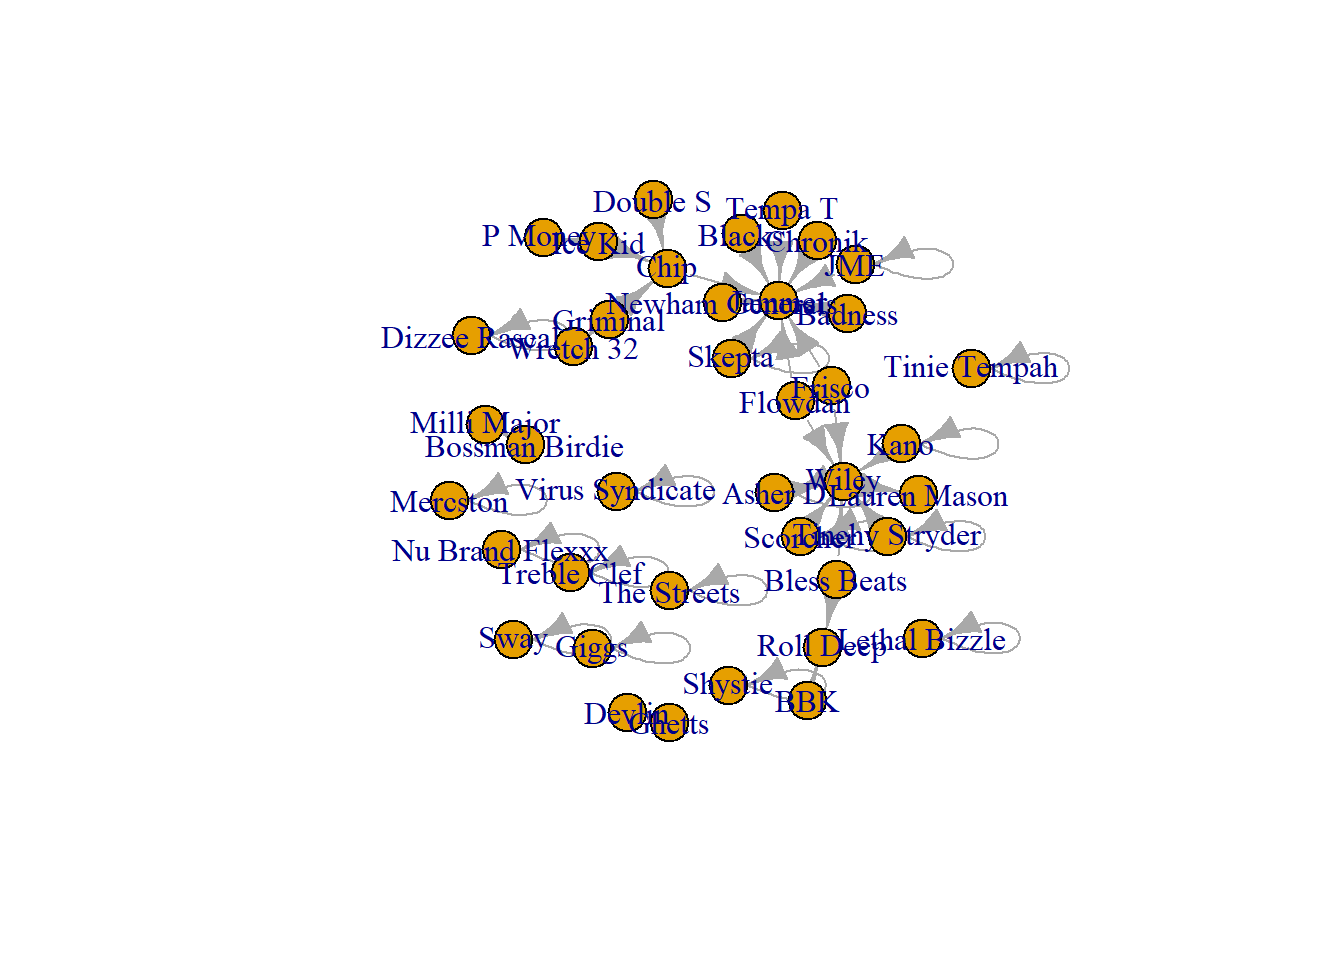
\includegraphics[keepaspectratio]{Basic-Visualisation_files/figure-pdf/unnamed-chunk-1-1.pdf}}

\begin{Shaded}
\begin{Highlighting}[]
\NormalTok{grime\_08\_clean }\OtherTok{\textless{}{-}} \FunctionTok{delete.edges}\NormalTok{(grime\_08, }\FunctionTok{E}\NormalTok{(grime\_08)[}\FunctionTok{which\_loop}\NormalTok{(grime\_08)])}

\FunctionTok{plot}\NormalTok{(grime\_08\_clean)}
\end{Highlighting}
\end{Shaded}

\pandocbounded{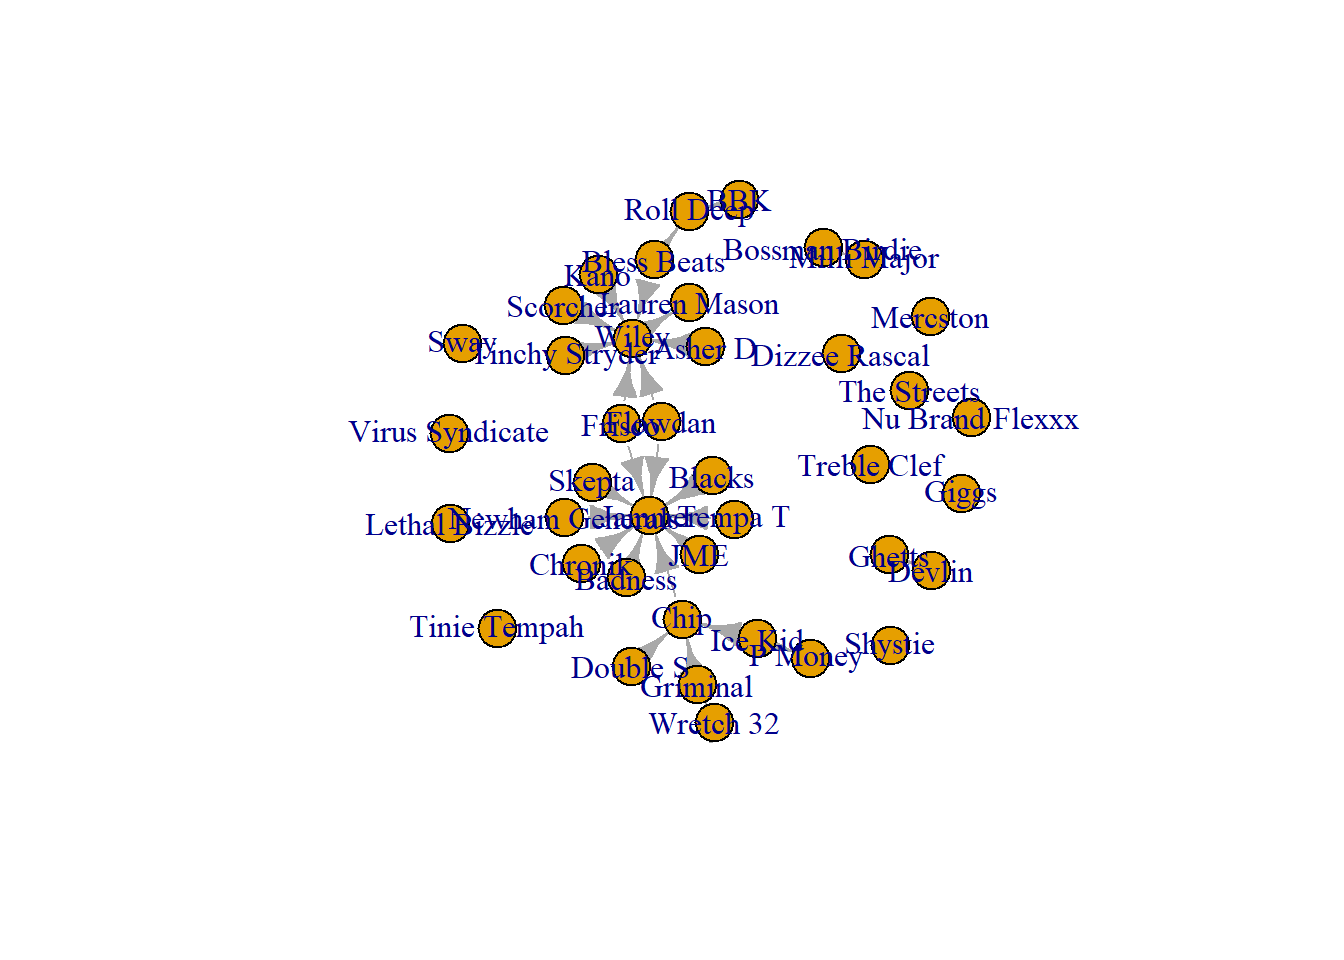
\includegraphics[keepaspectratio]{Basic-Visualisation_files/figure-pdf/unnamed-chunk-1-2.pdf}}

\section{Layout}\label{layout}

There are multiple preset layouts that igraph can deploy. Some layouts
emphasise the nodes in your graph (i.e.~making them clearer to see)
while others emphasise the edges. Take a look through each of these
layouts and see the types of stories you could tell about this network
with each.

\begin{itemize}
\tightlist
\item
  Random
\end{itemize}

\begin{Shaded}
\begin{Highlighting}[]
\FunctionTok{plot}\NormalTok{(grime\_08\_clean, }\AttributeTok{layout =}\NormalTok{ layout.random)}
\end{Highlighting}
\end{Shaded}

\pandocbounded{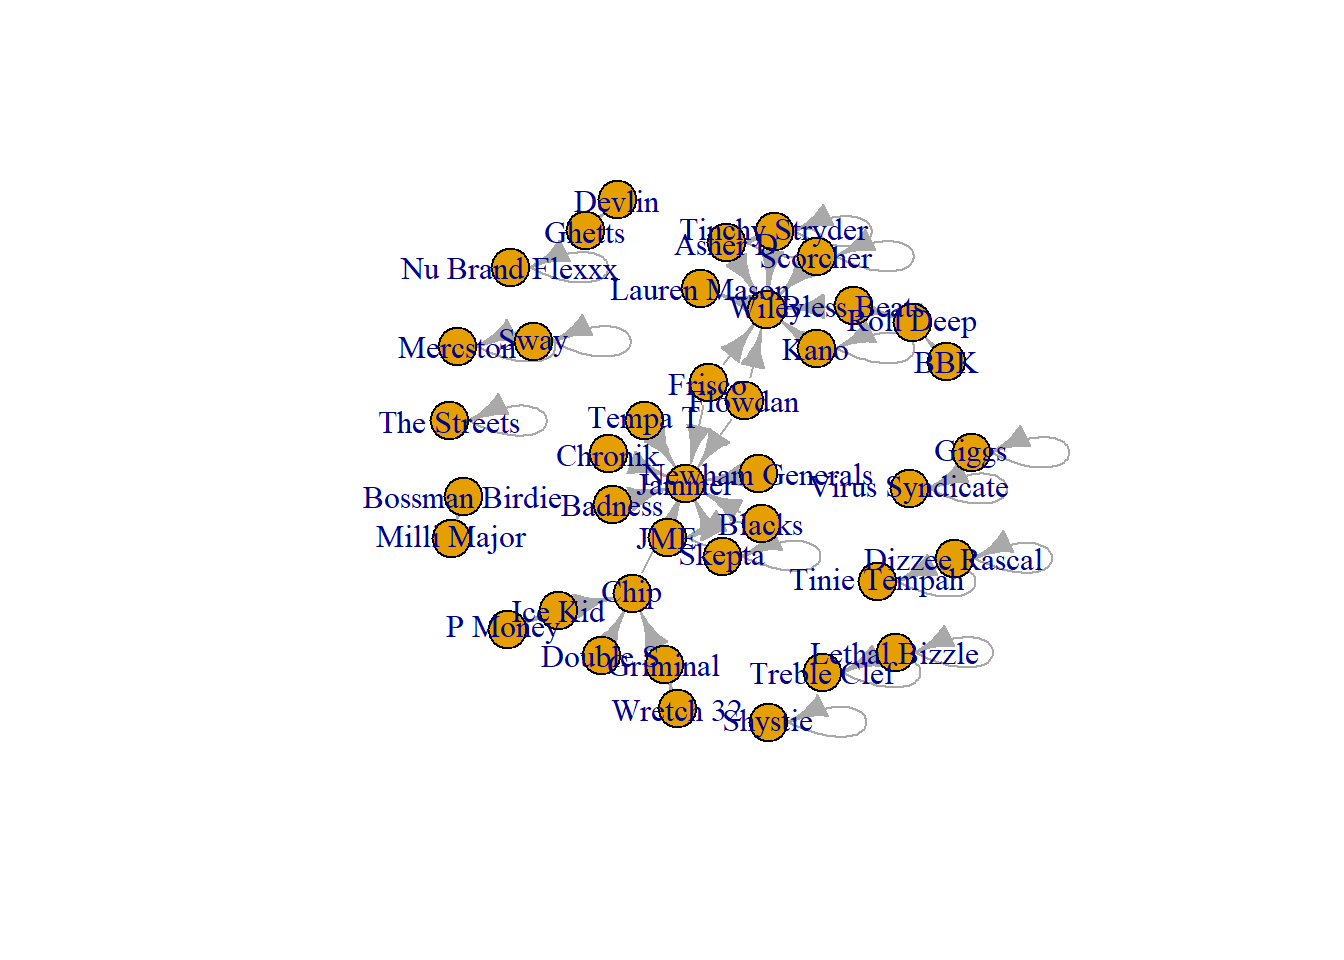
\includegraphics[keepaspectratio]{Basic-Visualisation_files/figure-pdf/unnamed-chunk-2-1.pdf}}

\begin{itemize}
\tightlist
\item
  Grid
\end{itemize}

\begin{Shaded}
\begin{Highlighting}[]
\FunctionTok{plot}\NormalTok{(grime\_08\_clean, }\AttributeTok{layout =}\NormalTok{ layout.grid)}
\end{Highlighting}
\end{Shaded}

\pandocbounded{\includegraphics[keepaspectratio]{Basic-Visualisation_files/figure-pdf/unnamed-chunk-3-1.pdf}}

\begin{itemize}
\tightlist
\item
  Small world/Circle
\end{itemize}

\begin{Shaded}
\begin{Highlighting}[]
\FunctionTok{plot}\NormalTok{(grime\_08\_clean, }\AttributeTok{layout =}\NormalTok{ layout.circle)}
\end{Highlighting}
\end{Shaded}

\pandocbounded{\includegraphics[keepaspectratio]{Basic-Visualisation_files/figure-pdf/unnamed-chunk-4-1.pdf}}

\begin{itemize}
\tightlist
\item
  Force-directed Layouts
\end{itemize}

These final layouts, called force-directed, determine the node's
position based on its relationship to others in the network. It attracts
a node towards those that they are connected to but ensures they do not
overlap. Here, we cover three algorithms, Fruchterman-Reingold,
Kamanda-Kawaii, and Davidson-Harl which all perform slightly
differently, but achieve the same thing.

\begin{Shaded}
\begin{Highlighting}[]
\FunctionTok{plot}\NormalTok{(grime\_08\_clean, }\AttributeTok{layout =} \FunctionTok{layout\_with\_dh}\NormalTok{(grime\_08\_clean))}
\end{Highlighting}
\end{Shaded}

\pandocbounded{\includegraphics[keepaspectratio]{Basic-Visualisation_files/figure-pdf/unnamed-chunk-5-1.pdf}}

\begin{Shaded}
\begin{Highlighting}[]
\FunctionTok{plot}\NormalTok{(grime\_08\_clean, }\AttributeTok{layout =} \FunctionTok{layout\_with\_fr}\NormalTok{(grime\_08\_clean))}
\end{Highlighting}
\end{Shaded}

\pandocbounded{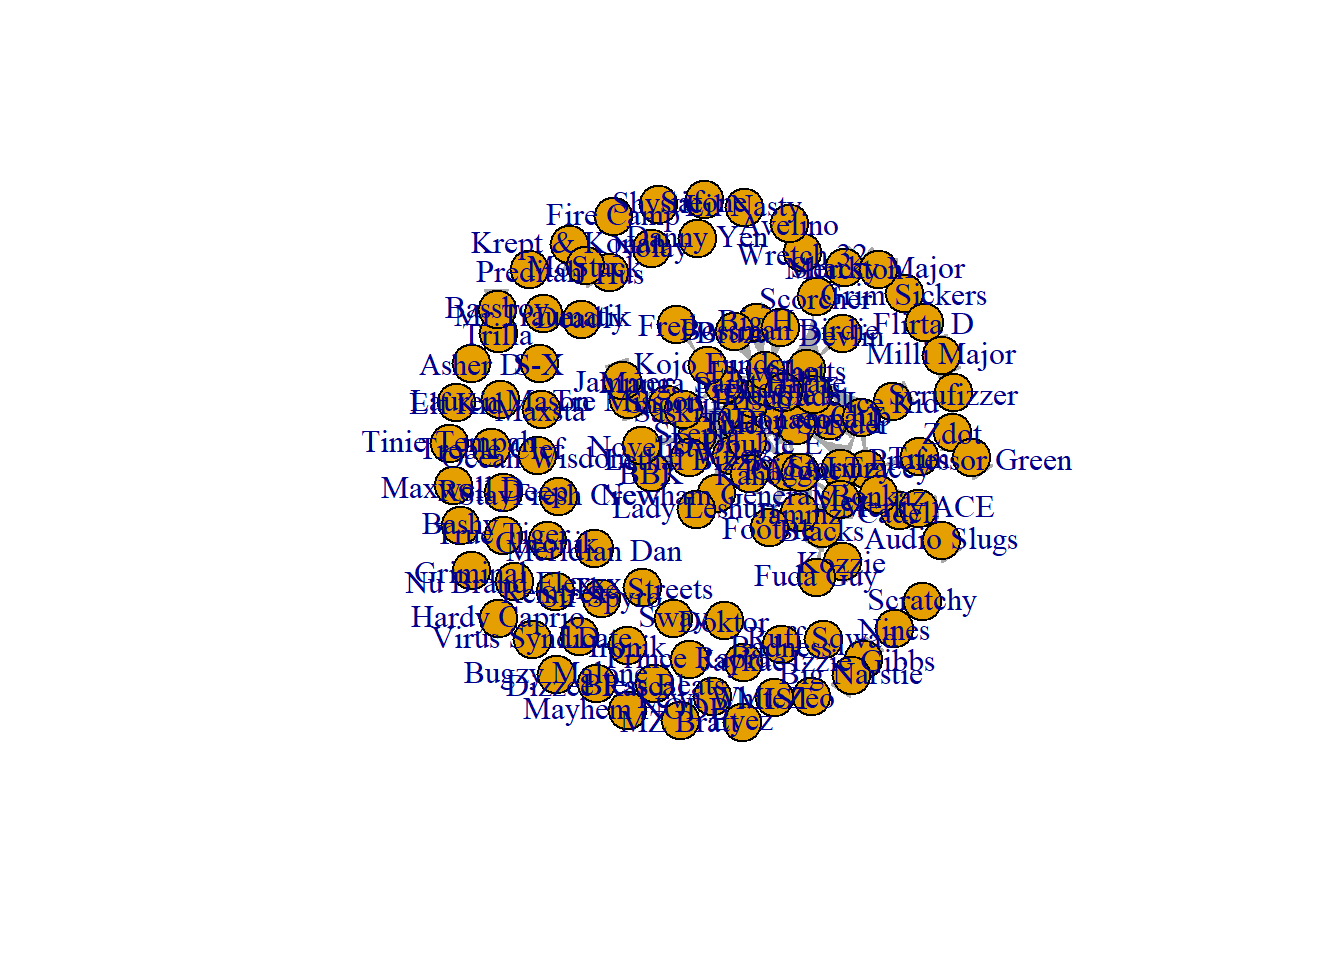
\includegraphics[keepaspectratio]{Basic-Visualisation_files/figure-pdf/unnamed-chunk-5-2.pdf}}

\begin{Shaded}
\begin{Highlighting}[]
\FunctionTok{plot}\NormalTok{(grime\_08\_clean, }\AttributeTok{layout =} \FunctionTok{layout\_with\_kk}\NormalTok{(grime\_08\_clean))}
\end{Highlighting}
\end{Shaded}

\pandocbounded{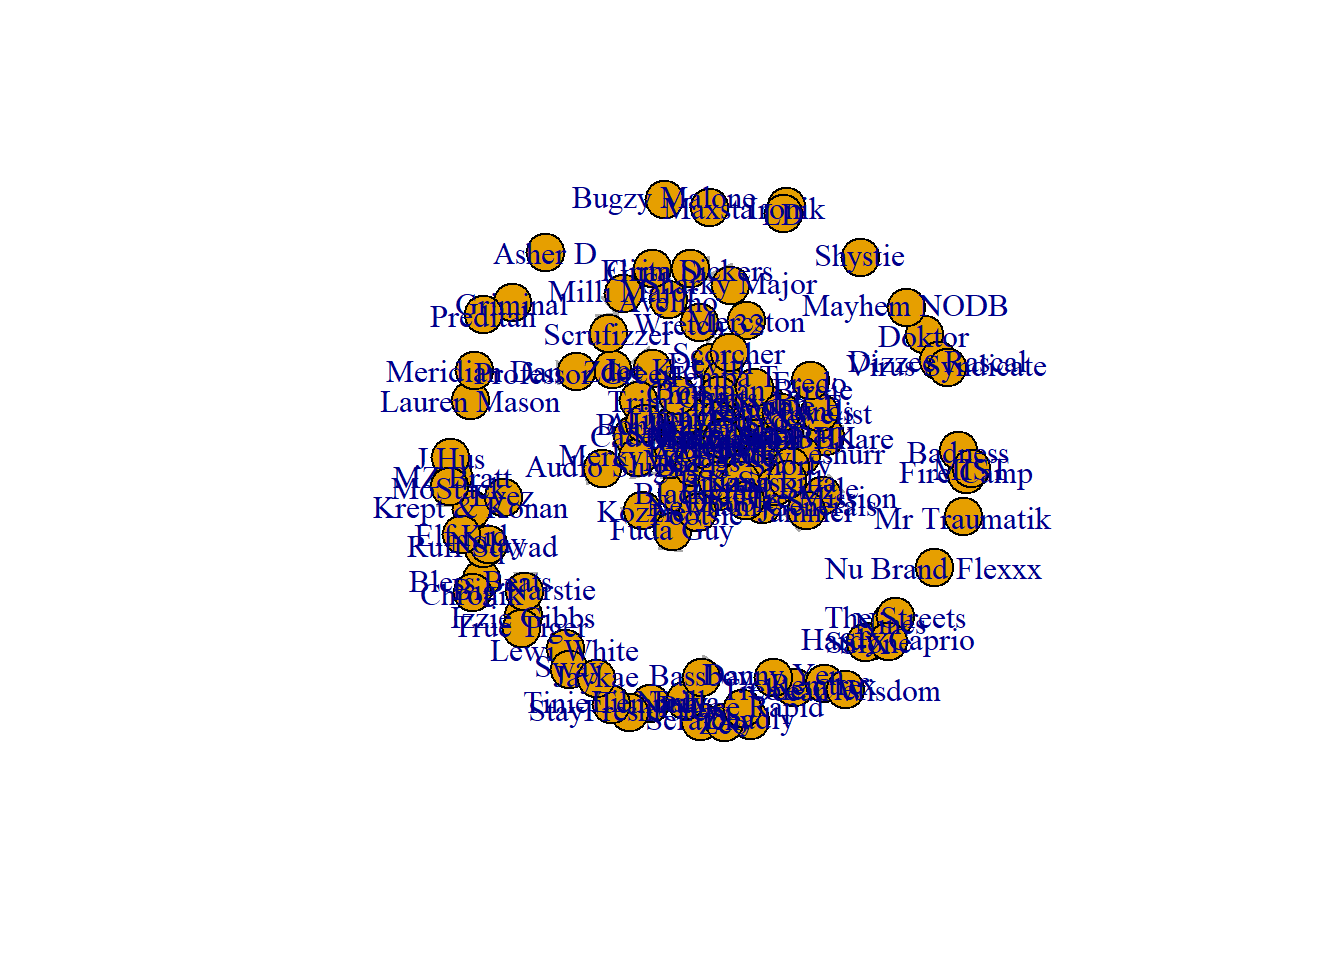
\includegraphics[keepaspectratio]{Basic-Visualisation_files/figure-pdf/unnamed-chunk-5-3.pdf}}

\section{Changing the Colours}\label{changing-the-colours}

Colours are an important aspect of network visualisation since they can
be used to distinguish one type of node from another, or they can be
used to accent certain nodes. However, remember that not everyone can
see colours clearly. Select colours that have a high contrast from one
another. In other words, colours that are distinct. Also, avoid colour
pairs that, commonly, colour blind people cannot differentiate. For
example, many can't differentiate between red and green. So, it is
advisable to avoid that pairing.

We can change the node colours with the verterx.color() option. You can
also toggle with the transparency of the colour using the adjustcolor
option and changing the colour's alpha. Adjusting the alpha can also
help with hairball visualisations since the transparency can help
visualise overlapping nodes.

\begin{Shaded}
\begin{Highlighting}[]
\FunctionTok{plot}\NormalTok{(grime\_08\_clean, }\AttributeTok{vertex.color =} \StringTok{"firebrick1"}\NormalTok{)}
\end{Highlighting}
\end{Shaded}

\pandocbounded{\includegraphics[keepaspectratio]{Basic-Visualisation_files/figure-pdf/unnamed-chunk-6-1.pdf}}

\begin{Shaded}
\begin{Highlighting}[]
\FunctionTok{plot}\NormalTok{(grime\_08\_clean, }\AttributeTok{vertex.color =} \FunctionTok{adjustcolor}\NormalTok{(}\StringTok{"firebrick1"}\NormalTok{, }\AttributeTok{alpha.f =} \FloatTok{0.5}\NormalTok{))}
\end{Highlighting}
\end{Shaded}

\pandocbounded{\includegraphics[keepaspectratio]{Basic-Visualisation_files/figure-pdf/unnamed-chunk-7-1.pdf}}

Edge colour with edge.color().

\begin{Shaded}
\begin{Highlighting}[]
\FunctionTok{plot}\NormalTok{(grime\_08\_clean, }\AttributeTok{edge.color =} \StringTok{"steelblue1"}\NormalTok{)}
\end{Highlighting}
\end{Shaded}

\pandocbounded{\includegraphics[keepaspectratio]{Basic-Visualisation_files/figure-pdf/unnamed-chunk-8-1.pdf}}

R recognises many of the common names or hex colours. See
\href{https://r-charts.com/colors/}{R-Charts} for more colours.

\section{Changing the Sizes}\label{changing-the-sizes}

You can change the sizes of various aspects of the graph to make it
clearer. Keep in mind that bigger does not always mean clearer! If you
have a network with a lot of nodes, the chances are that the nodes are
overlapping generating what we call a hairball. This is less than ideal
because hairballs actually hide any of the interesting structure that
exists within the network. Once way to overcome this is to make the edge
and vertex size smaller. Note that you may need to try different sizes
until you generate a clean visual.

\begin{Shaded}
\begin{Highlighting}[]
\FunctionTok{plot}\NormalTok{(grime\_08\_clean, }\AttributeTok{vertex.size =} \DecValTok{5}\NormalTok{, }\AttributeTok{edge.arrow.size =} \FloatTok{0.5}\NormalTok{)}
\end{Highlighting}
\end{Shaded}

\pandocbounded{\includegraphics[keepaspectratio]{Basic-Visualisation_files/figure-pdf/unnamed-chunk-9-1.pdf}}

Additionally, you can change the width of yours ties. While previously
we changed the size of the arrows themselves, below we change the width
of the lines.

\begin{Shaded}
\begin{Highlighting}[]
\FunctionTok{plot}\NormalTok{(grime\_08\_clean, }\AttributeTok{vertex.size =} \DecValTok{5}\NormalTok{, }\AttributeTok{edge.width =} \DecValTok{10}\NormalTok{)}
\end{Highlighting}
\end{Shaded}

\pandocbounded{\includegraphics[keepaspectratio]{Basic-Visualisation_files/figure-pdf/unnamed-chunk-10-1.pdf}}

\section{Titles}\label{titles}

Titles are a great way to further clarify your visualisation by making
it it easier to understand. Generally, there are two ``styles'' of
titles. The first is a little more academic that explains the
visualisation. Something like ``A Network Showing the Collaborations of
Grime Artists in 2008.'' This is very descriptive of that the graph is.
The second style is a more demonstrative of what the graph presents.
``Grime 2008 Had Two Well-Connected Artists.'' Rather than explaining
what the visualisation is (i.e.~a network) it explains what the graph
shows (i.e.~the story of the vis.). Be mindful of what audiences you are
creating visuals for. Are they interested more in explanation or the
story?

In Igraph, you can have a main title. This is usually at the head or top
of the network and orients people to your visual (in either style
discussed above).

\begin{Shaded}
\begin{Highlighting}[]
\FunctionTok{plot}\NormalTok{(grime\_08\_clean, }\AttributeTok{vertex.size =} \DecValTok{5}\NormalTok{, }\AttributeTok{edge.arrow.size =} \FloatTok{0.5}\NormalTok{, }\AttributeTok{main =} \StringTok{"A Networking Showing Grime Collaborations }\SpecialCharTok{\textbackslash{}n}\StringTok{ 2008"}\NormalTok{)}
\end{Highlighting}
\end{Shaded}

\pandocbounded{\includegraphics[keepaspectratio]{Basic-Visualisation_files/figure-pdf/unnamed-chunk-11-1.pdf}}

You may also wish to present a subtitle on your graph. Subtitles act as
footnotes or further explanations of your network. These titles are
usually placed at the foot (bottom) of your visualisation.

\begin{Shaded}
\begin{Highlighting}[]
\FunctionTok{plot}\NormalTok{(grime\_08\_clean, }\AttributeTok{vertex.size =} \DecValTok{5}\NormalTok{, }\AttributeTok{edge.arrow.size =} \FloatTok{0.5}\NormalTok{, }\AttributeTok{main =} \StringTok{"A Network Showing Grime Collaborations"}\NormalTok{, }\AttributeTok{sub =} \StringTok{"Year = 2008"}\NormalTok{)}
\end{Highlighting}
\end{Shaded}

\pandocbounded{\includegraphics[keepaspectratio]{Basic-Visualisation_files/figure-pdf/unnamed-chunk-12-1.pdf}}

\section{Labels}\label{labels}

Labeling nodes on your network can be useful so viewers can identify
nodes easily. Or, you can use them to draw people's attention to certain
nodes.

First, you may wish to change the size and offset the labels. These are
particularly useful if you have many labels that are running into each
other since reducing the size and offsetting them slightly can bring the
labels away from highly populated areas of the network increasing its
readability.

\begin{Shaded}
\begin{Highlighting}[]
\FunctionTok{plot}\NormalTok{(grime\_08\_clean, }\AttributeTok{vertex.label.cex =} \FloatTok{0.5}\NormalTok{, }\AttributeTok{vertex.label.dist =} \DecValTok{2}\NormalTok{)}
\end{Highlighting}
\end{Shaded}

\pandocbounded{\includegraphics[keepaspectratio]{Basic-Visualisation_files/figure-pdf/unnamed-chunk-13-1.pdf}}

Alternatively, you may wish to remove the labels altogether. This is
useful if you have many nodes and the node labels are running into each
other regardless of your sizing and offsetting.

\begin{Shaded}
\begin{Highlighting}[]
\FunctionTok{plot}\NormalTok{(grime\_08\_clean, }\AttributeTok{vertex.label =} \ConstantTok{NA}\NormalTok{)}
\end{Highlighting}
\end{Shaded}

\pandocbounded{\includegraphics[keepaspectratio]{Basic-Visualisation_files/figure-pdf/unnamed-chunk-14-1.pdf}}

Finally, you may wish to present the labels of highly connected
individuals in the network. Here, for example, we have a slightly more
advanced visualisation to demonstrate the well-connected artists in the
network. See if you can follow the logic of the code.

\begin{Shaded}
\begin{Highlighting}[]
\FunctionTok{plot}\NormalTok{(grime\_08\_clean, }\AttributeTok{vertex.label =} \FunctionTok{ifelse}\NormalTok{(}\FunctionTok{degree}\NormalTok{(grime\_08\_clean) }\SpecialCharTok{\textgreater{}} \DecValTok{4}\NormalTok{, }\FunctionTok{V}\NormalTok{(grime\_08\_clean)}\SpecialCharTok{$}\NormalTok{name, }\ConstantTok{NA}\NormalTok{), }\AttributeTok{vertex.label.cex =} \FloatTok{0.5}\NormalTok{, }\AttributeTok{vertex.label.color =} \StringTok{"white"}\NormalTok{, }\AttributeTok{vertex.color =} \FunctionTok{ifelse}\NormalTok{(}\FunctionTok{degree}\NormalTok{(grime\_08\_clean) }\SpecialCharTok{\textgreater{}} \DecValTok{4}\NormalTok{, }\StringTok{"purple"}\NormalTok{, }\StringTok{"green"}\NormalTok{), }\AttributeTok{vertex.size =} \DecValTok{10}\NormalTok{, }\AttributeTok{edge.arrow.size =} \FloatTok{0.25}\NormalTok{)}
\end{Highlighting}
\end{Shaded}

\pandocbounded{\includegraphics[keepaspectratio]{Basic-Visualisation_files/figure-pdf/unnamed-chunk-15-1.pdf}}

Here, then, we combine multiple visualisation techniques to generate a
clean visualisation that emphasises the two most highly connected
artists in Grime during 2008, Wiley and Jammer. We have changed the
colour of the nodes in the graph to purple if they have more than 4
connections and greenif they have less. Since we are discussing a labels
here, pay special attention to the ifelse() statement for the vertex
label. We have changed the labels to show only those with more than 4
connections. Due to the node colour being dark, we also set the label
colour to white.

\section{General considerations for
visualizations}\label{general-considerations-for-visualizations}

So, we have talked about changing specific elements of your
visualisation to clean it by reducing the visual noise and maximising
certain aspects of the graph we care about. However, there are a few
other tricks that you can use in R to help producing your
visualisations.

\begin{enumerate}
\def\labelenumi{\arabic{enumi}.}
\tightlist
\item
  The Aspect Ratio
\end{enumerate}

At the moment, the plots we have created look rather ``zoomed out.''
Almost as though you are looking at it through the wrong end of
binoculars. This is because RStudio has margins on their plot windows.
What that means is that there is a standard set amount of white space
along the margins (sides, top and bottom) of a plot. We can reduce these
margins with the par() function and reduce the margins (mar=) to 0. What
this effectively does is ``zoom in'' to the plot by removing the white
space. Bare in mind, the mar option starts at the bottom, left, top,
then right. So, if you have a mar = c(5,1,1,3) you will have a plot that
has five units on the bottom, 1 on the left and top, then 3 on the
right. You must run the par() function prior to your plot() for it to
take effect. Take a look at the following plots for a demonstration.

\begin{Shaded}
\begin{Highlighting}[]
\FunctionTok{plot}\NormalTok{(grime\_08\_clean, }\AttributeTok{vertex.label =} \ConstantTok{NA}\NormalTok{)}
\end{Highlighting}
\end{Shaded}

\pandocbounded{\includegraphics[keepaspectratio]{Basic-Visualisation_files/figure-pdf/unnamed-chunk-16-1.pdf}}

\begin{Shaded}
\begin{Highlighting}[]
\FunctionTok{par}\NormalTok{(}\AttributeTok{mar =}\FunctionTok{c}\NormalTok{(}\DecValTok{0}\NormalTok{,}\DecValTok{0}\NormalTok{,}\DecValTok{0}\NormalTok{,}\DecValTok{0}\NormalTok{))}

\FunctionTok{plot}\NormalTok{(grime\_08\_clean, }\AttributeTok{vertex.label =} \ConstantTok{NA}\NormalTok{)}
\end{Highlighting}
\end{Shaded}

\pandocbounded{\includegraphics[keepaspectratio]{Basic-Visualisation_files/figure-pdf/unnamed-chunk-16-2.pdf}}

We have reduced the margins all down to zero in the second plot. Keep in
mind, if you have titles (main or sub) or a key/legend on your plotm you
will need to increase the margins accordingly since they are placed into
the margins.

\begin{enumerate}
\def\labelenumi{\arabic{enumi}.}
\setcounter{enumi}{1}
\tightlist
\item
  Replicating Plots - set.seed()
\end{enumerate}

You might have noticed that each time we plot our grime network, it
looks a little different. The nodes and edges are all the same but the
position of the visualisation is different each time. This occurs
because R begins a plot from a point (think coordinates) in the plot
window and selects a different place each time. In order to produce the
same plot more than once, you must set the seed which basically means
telling R where to start. If it starts in the same place each time, it
will produce the same visual. Take a look at the following code.

\begin{Shaded}
\begin{Highlighting}[]
\FunctionTok{par}\NormalTok{(}\AttributeTok{mar =}\FunctionTok{c}\NormalTok{(}\DecValTok{0}\NormalTok{,}\DecValTok{0}\NormalTok{,}\DecValTok{0}\NormalTok{,}\DecValTok{0}\NormalTok{))}
\FunctionTok{set.seed}\NormalTok{(}\DecValTok{123}\NormalTok{)}
\FunctionTok{plot}\NormalTok{(grime\_08\_clean, }\AttributeTok{vertex.label =} \ConstantTok{NA}\NormalTok{)}
\end{Highlighting}
\end{Shaded}

\pandocbounded{\includegraphics[keepaspectratio]{Basic-Visualisation_files/figure-pdf/unnamed-chunk-17-1.pdf}}

In the above chunk we have set the parameters (zoomed in) and selected a
seed (starting point) of 123. This could be whatever numbers you want.
So long as you call on it the same each time you plot that network, it
will produce the same visual. See below, for example.

\begin{Shaded}
\begin{Highlighting}[]
\FunctionTok{par}\NormalTok{(}\AttributeTok{mar =}\FunctionTok{c}\NormalTok{(}\DecValTok{0}\NormalTok{,}\DecValTok{0}\NormalTok{,}\DecValTok{0}\NormalTok{,}\DecValTok{0}\NormalTok{))}
\FunctionTok{set.seed}\NormalTok{(}\DecValTok{123}\NormalTok{)}
\FunctionTok{plot}\NormalTok{(grime\_08\_clean, }\AttributeTok{vertex.label =} \ConstantTok{NA}\NormalTok{)}
\end{Highlighting}
\end{Shaded}

\pandocbounded{\includegraphics[keepaspectratio]{Basic-Visualisation_files/figure-pdf/unnamed-chunk-18-1.pdf}}

The visualisation is replicated. This is particularly useful when you
need to produce the same visual (i.e.~for a publication). So, when you
care about reproducing the network visual, set the seed!

\begin{enumerate}
\def\labelenumi{\arabic{enumi}.}
\setcounter{enumi}{2}
\tightlist
\item
  Multiple Plots
\end{enumerate}

One final trick, you may want to have more than one plot next to each
other. This side-by-side approach is often used to compare across
visualisations or to present different elements of the network. Again,
we use the par() function, but this time we use the mfrow option and
then set the number of rows and columns in our plot.

Here we set our plot to have two rows and one column which presents one
visual stacked on the other.

\begin{Shaded}
\begin{Highlighting}[]
\FunctionTok{par}\NormalTok{(}\AttributeTok{mfrow =} \FunctionTok{c}\NormalTok{(}\DecValTok{2}\NormalTok{, }\DecValTok{1}\NormalTok{))}

\FunctionTok{par}\NormalTok{(}\AttributeTok{mar =}\FunctionTok{c}\NormalTok{(}\DecValTok{0}\NormalTok{,}\DecValTok{0}\NormalTok{,}\DecValTok{0}\NormalTok{,}\DecValTok{0}\NormalTok{))}

\FunctionTok{set.seed}\NormalTok{(}\DecValTok{123}\NormalTok{)}
\FunctionTok{plot}\NormalTok{(grime\_08\_clean, }\AttributeTok{vertex.label =} \ConstantTok{NA}\NormalTok{)}

\FunctionTok{set.seed}\NormalTok{(}\DecValTok{123}\NormalTok{)}
\FunctionTok{par}\NormalTok{(}\AttributeTok{mar =}\FunctionTok{c}\NormalTok{(}\DecValTok{0}\NormalTok{,}\DecValTok{0}\NormalTok{,}\DecValTok{0}\NormalTok{,}\DecValTok{0}\NormalTok{))}
\FunctionTok{plot}\NormalTok{(grime\_08\_clean, }\AttributeTok{vertex.label =} \FunctionTok{ifelse}\NormalTok{(}\FunctionTok{degree}\NormalTok{(grime\_08\_clean) }\SpecialCharTok{\textgreater{}} \DecValTok{4}\NormalTok{, }\FunctionTok{V}\NormalTok{(grime\_08\_clean)}\SpecialCharTok{$}\NormalTok{name, }\ConstantTok{NA}\NormalTok{), }\AttributeTok{vertex.label.cex =} \FloatTok{0.5}\NormalTok{, }\AttributeTok{vertex.label.color =} \StringTok{"white"}\NormalTok{, }\AttributeTok{vertex.color =} \FunctionTok{ifelse}\NormalTok{(}\FunctionTok{degree}\NormalTok{(grime\_08\_clean) }\SpecialCharTok{\textgreater{}} \DecValTok{4}\NormalTok{, }\StringTok{"purple"}\NormalTok{, }\StringTok{"green"}\NormalTok{), }\AttributeTok{vertex.size =} \DecValTok{10}\NormalTok{, }\AttributeTok{edge.arrow.size =} \FloatTok{0.25}\NormalTok{)}
\end{Highlighting}
\end{Shaded}

\pandocbounded{\includegraphics[keepaspectratio]{Basic-Visualisation_files/figure-pdf/unnamed-chunk-19-1.pdf}}

Or, if we flip the rows and columns, we end up with a side-by-side plot.

\begin{Shaded}
\begin{Highlighting}[]
\FunctionTok{par}\NormalTok{(}\AttributeTok{mfrow =} \FunctionTok{c}\NormalTok{(}\DecValTok{1}\NormalTok{, }\DecValTok{2}\NormalTok{))}
\FunctionTok{set.seed}\NormalTok{(}\DecValTok{123}\NormalTok{)}
\FunctionTok{par}\NormalTok{(}\AttributeTok{mar =}\FunctionTok{c}\NormalTok{(}\DecValTok{0}\NormalTok{,}\DecValTok{0}\NormalTok{,}\DecValTok{0}\NormalTok{,}\DecValTok{0}\NormalTok{))}
\FunctionTok{plot}\NormalTok{(grime\_08\_clean, }\AttributeTok{vertex.label =} \ConstantTok{NA}\NormalTok{)}

\FunctionTok{set.seed}\NormalTok{(}\DecValTok{123}\NormalTok{)}
\FunctionTok{par}\NormalTok{(}\AttributeTok{mar =}\FunctionTok{c}\NormalTok{(}\DecValTok{0}\NormalTok{,}\DecValTok{0}\NormalTok{,}\DecValTok{0}\NormalTok{,}\DecValTok{0}\NormalTok{))}
\FunctionTok{plot}\NormalTok{(grime\_08\_clean, }\AttributeTok{vertex.label =} \FunctionTok{ifelse}\NormalTok{(}\FunctionTok{degree}\NormalTok{(grime\_08\_clean) }\SpecialCharTok{\textgreater{}} \DecValTok{4}\NormalTok{, }\FunctionTok{V}\NormalTok{(grime\_08\_clean)}\SpecialCharTok{$}\NormalTok{name, }\ConstantTok{NA}\NormalTok{), }\AttributeTok{vertex.label.cex =} \FloatTok{0.5}\NormalTok{, }\AttributeTok{vertex.label.color =} \StringTok{"white"}\NormalTok{, }\AttributeTok{vertex.color =} \FunctionTok{ifelse}\NormalTok{(}\FunctionTok{degree}\NormalTok{(grime\_08\_clean) }\SpecialCharTok{\textgreater{}} \DecValTok{4}\NormalTok{, }\StringTok{"purple"}\NormalTok{, }\StringTok{"green"}\NormalTok{), }\AttributeTok{vertex.size =} \DecValTok{10}\NormalTok{, }\AttributeTok{edge.arrow.size =} \FloatTok{0.25}\NormalTok{)}
\end{Highlighting}
\end{Shaded}

\pandocbounded{\includegraphics[keepaspectratio]{Basic-Visualisation_files/figure-pdf/unnamed-chunk-20-1.pdf}}

\section{Summary}\label{summary-6}

Visualisation is a powerful tool to communicate data. However,
visualisations can be very messy and the mess may confuse rather than
clarify. In this section, we have covered:

\begin{enumerate}
\def\labelenumi{\arabic{enumi}.}
\tightlist
\item
  Methods for reducing visual noise in a network through changing the
  layout, sizes, and colours
\item
  Effective titling methods
\item
  Ways to make certain aspects of the network more prominent
\item
  Effective and accessible collouring of network visualisations
\item
  General tricks for creating network visuals in RStudio.
\end{enumerate}

Well done!

\chapter{Visualisations -
Intermediate}\label{visualisations---intermediate}

\begin{Shaded}
\begin{Highlighting}[]
\FunctionTok{library}\NormalTok{(igraph)}
\FunctionTok{library}\NormalTok{(ADAPTSNA)}
\end{Highlighting}
\end{Shaded}

In the previous chapter, we talked about creating clean network visuals
that are sized and proportioned well enough so as to reduce the visual
noise of networks. Here, we take a step further and focus on telling a
story through network visualisation.

\begin{longtable}[]{@{}
  >{\raggedright\arraybackslash}p{(\linewidth - 0\tabcolsep) * \real{1.0057}}@{}}
\toprule\noalign{}
\begin{minipage}[b]{\linewidth}\raggedright
LEARNING ELEMENTS - Data Practices
\end{minipage} \\
\midrule\noalign{}
\endhead
\bottomrule\noalign{}
\endlastfoot
\begin{minipage}[t]{\linewidth}\raggedright
\begin{itemize}
\tightlist
\item
  Stories in Data. One main purpose of visualisation is to tell a story
  to your constituents. Here you will learn how to produce network
  visualisations that tell a story.
\end{itemize}
\end{minipage} \\
\end{longtable}

First, bring in the data on Grime musicians and their collaborations
with each other in 2008. Then clean the network a little bit by deleting
the self-loops.

\begin{Shaded}
\begin{Highlighting}[]
\NormalTok{grime\_edge\_list }\OtherTok{\textless{}{-}} \FunctionTok{load\_data}\NormalTok{(}\StringTok{"GRIME\_2008\_Edge.csv"}\NormalTok{, }\AttributeTok{header =} \ConstantTok{TRUE}\NormalTok{) }

\NormalTok{grime\_08 }\OtherTok{\textless{}{-}} \FunctionTok{graph\_from\_data\_frame}\NormalTok{(}\AttributeTok{d=}\NormalTok{ grime\_edge\_list, }\AttributeTok{directed =} \ConstantTok{TRUE}\NormalTok{)}
\FunctionTok{plot}\NormalTok{(grime\_08)}
\end{Highlighting}
\end{Shaded}

\pandocbounded{\includegraphics[keepaspectratio]{Intermediate-Visualisation_files/figure-pdf/unnamed-chunk-2-1.pdf}}

\begin{Shaded}
\begin{Highlighting}[]
\NormalTok{grime\_08\_clean }\OtherTok{\textless{}{-}} \FunctionTok{delete.edges}\NormalTok{(grime\_08, }\FunctionTok{E}\NormalTok{(grime\_08)[}\FunctionTok{which\_loop}\NormalTok{(grime\_08)])}

\FunctionTok{plot}\NormalTok{(grime\_08\_clean)}
\end{Highlighting}
\end{Shaded}

\pandocbounded{\includegraphics[keepaspectratio]{Intermediate-Visualisation_files/figure-pdf/unnamed-chunk-2-2.pdf}}

Now we are ready to start our storytelling in networks! We can produce
visualisations that tell a story about the individuals in the network
and the relationships that exist between them. In general, you can alter
the network visualisation's characteristics to tell a story.

The network contains information about the individuals that we can draw
out in our visualisation. This information is based on the relationships
they have with others in the network.

\section{Visualising Prominent and Influential
Nodes}\label{visualising-prominent-and-influential-nodes}

There are multiple measurements of centrality and we will cover more of
them in \href{People\%20In\%20Networks.qmd}{Chapter 16}. For now, we
will create visualisations aimed at highlighting prominent and
influential nodes in the network using two measures of centrality,
degree and betweenness. For more on those measures, hand tight and read
later chapters.

For now, consider centrality as a way of understanding an individual's
position within a network. You may have heard someone described as
``well-connected''---a phrase that typically refers to a person's
influence, power, or popularity within a social context. Centrality
measures, grounded in graph theory, provide a formal means of
quantifying this idea.

Individuals with many direct connections---those with high degree
centrality---are considered \emph{prominent} because they maintain
relationships with numerous others in the network. Their visibility and
accessibility position them at the center of group interactions. In
contrast, individuals with high \emph{betweenness centrality}---those
who frequently lie on the shortest paths between others---are described
as \emph{influential}. This is because they occupy strategic bridging
positions that allow them to mediate, facilitate, or even control the
flow of information or resources across the network.

\subsection{Prominence}\label{prominence}

There are two main ways that we can demonstrate a node's prominence or
influence in a network. We could alter the size of the nodes to be
commensurate to their score. So, if a node has a degree centrality of
10, their size would be 10 compared to another node with a score (and
therefore node size) of 5. The difference in size is useful to
demonstrate that one is more prominent than the other. Alternatively, we
could change the labels to reflect those scores.

\begin{Shaded}
\begin{Highlighting}[]
\FunctionTok{par}\NormalTok{(}\AttributeTok{mar =} \FunctionTok{c}\NormalTok{(}\DecValTok{5}\NormalTok{,}\DecValTok{0}\NormalTok{,}\DecValTok{0}\NormalTok{,}\DecValTok{0}\NormalTok{))}
\FunctionTok{plot}\NormalTok{(grime\_08\_clean, }\AttributeTok{vertex.size =} \FunctionTok{degree}\NormalTok{(grime\_08\_clean)}\SpecialCharTok{*}\DecValTok{2}\NormalTok{, }\AttributeTok{edge.arrow.size =} \FloatTok{0.5}\NormalTok{, }\AttributeTok{sub =} \StringTok{"Node Size Presents More Prominent Artists"}\NormalTok{)}
\end{Highlighting}
\end{Shaded}

\pandocbounded{\includegraphics[keepaspectratio]{Intermediate-Visualisation_files/figure-pdf/unnamed-chunk-3-1.pdf}}

What does the above visualisation tell you about this network? Who are
the most/more prominent artists in this network?

Based on that network we can clearly see two artists `pop' from the
visualisation more than others. This suggests that this group has two
very prominent artists.

An issue with using node size to generate comparisons between nodes is
that seeing the difference between someone who has a score of 9 compared
to 10 might be difficult since they are close in size. A workaround is
to use the node labels to reflect the score. That way people can read
the scores directly.

\begin{Shaded}
\begin{Highlighting}[]
\FunctionTok{par}\NormalTok{(}\AttributeTok{mar =} \FunctionTok{c}\NormalTok{(}\DecValTok{0}\NormalTok{,}\DecValTok{0}\NormalTok{,}\DecValTok{0}\NormalTok{,}\DecValTok{0}\NormalTok{)) }
\FunctionTok{plot}\NormalTok{(grime\_08\_clean, }\AttributeTok{vertex.label =} \FunctionTok{degree}\NormalTok{(grime\_08\_clean))}
\end{Highlighting}
\end{Shaded}

\pandocbounded{\includegraphics[keepaspectratio]{Intermediate-Visualisation_files/figure-pdf/unnamed-chunk-4-1.pdf}}

This tells the same information as the first visual. However, there are
some pros and cons to this approach. The positives are that viewers can
easily see the differences in scores. The drawbacks are that it produces
a slightly more noisy visualisation. A viewer will neet to look through
the whole network to identify those with high scores. With this network,
it might be better to use the size since the visual looks a little
cleaner. As always, trial and error! Give both a go and see what works
better. Or, present both!

\subsection{Influence}\label{influence}

Next, we can do the same thing to demonstrate influential individuals in
this network.

\begin{Shaded}
\begin{Highlighting}[]
\FunctionTok{par}\NormalTok{(}\AttributeTok{mar =} \FunctionTok{c}\NormalTok{(}\DecValTok{0}\NormalTok{,}\DecValTok{0}\NormalTok{,}\DecValTok{0}\NormalTok{,}\DecValTok{0}\NormalTok{))}
\FunctionTok{plot}\NormalTok{(grime\_08\_clean, }\AttributeTok{vertex.size =} \FunctionTok{betweenness}\NormalTok{(grime\_08\_clean)}\SpecialCharTok{*}\DecValTok{2}\NormalTok{, }\AttributeTok{edge.arrow.size =} \FloatTok{0.5}\NormalTok{)}
\end{Highlighting}
\end{Shaded}

\pandocbounded{\includegraphics[keepaspectratio]{Intermediate-Visualisation_files/figure-pdf/unnamed-chunk-5-1.pdf}}

Again the same limitations and strengths apply here as they do when
visualising prominence.

\begin{Shaded}
\begin{Highlighting}[]
\FunctionTok{par}\NormalTok{(}\AttributeTok{mar =} \FunctionTok{c}\NormalTok{(}\DecValTok{0}\NormalTok{,}\DecValTok{0}\NormalTok{,}\DecValTok{0}\NormalTok{,}\DecValTok{0}\NormalTok{))}
\FunctionTok{plot}\NormalTok{(grime\_08\_clean, }\AttributeTok{vertex.label =} \FunctionTok{betweenness}\NormalTok{(grime\_08\_clean))}
\end{Highlighting}
\end{Shaded}

\pandocbounded{\includegraphics[keepaspectratio]{Intermediate-Visualisation_files/figure-pdf/unnamed-chunk-6-1.pdf}}

Notice here, that there different artists appear to be influential that
are not very prominent and some that are prominent but not influential.
This has to do with the differences between the measures since they
capture different things. Again, for more on this, read
\href{People\%20In\%20Networks.qmd}{Chapter 16}.

\section{Visualising Relationships}\label{visualising-relationships}

Next, providing we have the information, we can tell stories about the
relationships that exist between nodes. This section relies on the
assumption that the network has information about the edges. We have
already covered a few things (see
\href{Node\%20and\%20Edge\%20Attributes.qmd}{Chapter 7}) but will go
over a few other things here. In this network we have an edge weight
that reflects the number of collaborations that the artists have had.
Again, you can change the size (width) of the edge or add labels to the
edge that reflects the edge weight.

Here, thicker edgest reflect more collaborations between the artists.
This clearly demonstrates connections in the network that are `stronger'
than others.

\begin{Shaded}
\begin{Highlighting}[]
\FunctionTok{par}\NormalTok{(}\AttributeTok{mar =} \FunctionTok{c}\NormalTok{(}\DecValTok{0}\NormalTok{,}\DecValTok{0}\NormalTok{,}\DecValTok{0}\NormalTok{,}\DecValTok{0}\NormalTok{))}
\FunctionTok{plot}\NormalTok{(grime\_08\_clean, }\AttributeTok{edge.width =} \FunctionTok{E}\NormalTok{(grime\_08\_clean)}\SpecialCharTok{$}\NormalTok{collab\_weight, }\AttributeTok{edge.arrow.size =} \FloatTok{0.5}\NormalTok{, }\AttributeTok{vertex.size =} \DecValTok{6}\NormalTok{, }\AttributeTok{vertex.label =} \ConstantTok{NA}\NormalTok{)}
\end{Highlighting}
\end{Shaded}

\pandocbounded{\includegraphics[keepaspectratio]{Intermediate-Visualisation_files/figure-pdf/unnamed-chunk-7-1.pdf}}

The labels provide the exact amount. You might consider showing the
labels of only those what have a certain (or higher than a certain)
amount since showing labels on all edges gets a bit noisy.

\begin{Shaded}
\begin{Highlighting}[]
\FunctionTok{par}\NormalTok{(}\AttributeTok{mar =} \FunctionTok{c}\NormalTok{(}\DecValTok{0}\NormalTok{,}\DecValTok{0}\NormalTok{,}\DecValTok{0}\NormalTok{,}\DecValTok{0}\NormalTok{))}
\FunctionTok{plot}\NormalTok{(grime\_08\_clean, }\AttributeTok{edge.width =} \FunctionTok{E}\NormalTok{(grime\_08\_clean)}\SpecialCharTok{$}\NormalTok{collab\_weight, }\AttributeTok{edge.label =} \FunctionTok{E}\NormalTok{(grime\_08\_clean)}\SpecialCharTok{$}\NormalTok{collab\_weight, }\AttributeTok{edge.arrow.size =} \FloatTok{0.5}\NormalTok{, }\AttributeTok{vertex.size =} \DecValTok{6}\NormalTok{, }\AttributeTok{vertex.label =} \ConstantTok{NA}\NormalTok{) }
\end{Highlighting}
\end{Shaded}

\pandocbounded{\includegraphics[keepaspectratio]{Intermediate-Visualisation_files/figure-pdf/unnamed-chunk-8-1.pdf}}

\section{Node Level Characteristics}\label{node-level-characteristics}

Finally, you can combine node-level characteristics with these other
visualisations to tell more stories in your visualisation.

Here, I attach data external to the network (i.e.~node characteristics)
and visualise those. I bring in a separate .csv file that has various
variables that pertain to the nodes. \textbf{These are fake
characteristics that I made up.} Take a look at this to see what we have
available. 2 variables - fake sales (continuous) and the artist's sex
(categorical - dichotomous)

\begin{Shaded}
\begin{Highlighting}[]
\NormalTok{grime\_nodes }\OtherTok{\textless{}{-}} \FunctionTok{load\_data}\NormalTok{(}\StringTok{"GRIME\_2008\_Nodes.csv"}\NormalTok{)}
\FunctionTok{head}\NormalTok{(grime\_nodes)}
\end{Highlighting}
\end{Shaded}

\begin{verbatim}
           node fake_sales sex
1       Asher D         10   m
2 Dizzee Rascal         20   m
3 Lethal Bizzle         50   m
4         Wiley         70   m
5   Treble Clef        100   m
6       Shystie         95   f
\end{verbatim}

Now we can create a network object that has both the network data and
the node characteristics. This section uses the vertices = argument
which tells R that there are edges and node characteristics as part of
the network. I also clean the selfloops from this edgelist.

\begin{Shaded}
\begin{Highlighting}[]
\NormalTok{grime\_full }\OtherTok{\textless{}{-}} \FunctionTok{graph\_from\_data\_frame}\NormalTok{(grime\_edge\_list, }\AttributeTok{vertices =}\NormalTok{ grime\_nodes, }\AttributeTok{directed =} \ConstantTok{TRUE}\NormalTok{)}
\NormalTok{grime\_full\_clean }\OtherTok{\textless{}{-}} \FunctionTok{delete.edges}\NormalTok{(grime\_full, }\FunctionTok{E}\NormalTok{(grime\_full)[}\FunctionTok{which\_loop}\NormalTok{(grime\_full)])}
\end{Highlighting}
\end{Shaded}

We can use these node attributes to visualise more about the network

\begin{Shaded}
\begin{Highlighting}[]
\NormalTok{sex }\OtherTok{\textless{}{-}}\FunctionTok{ifelse}\NormalTok{(}\FunctionTok{V}\NormalTok{(grime\_full\_clean)}\SpecialCharTok{$}\NormalTok{sex }\SpecialCharTok{==} \StringTok{"f"}\NormalTok{, }\StringTok{"red"}\NormalTok{, }\StringTok{"white"}\NormalTok{)}

\FunctionTok{par}\NormalTok{(}\AttributeTok{mar =} \FunctionTok{c}\NormalTok{(}\DecValTok{0}\NormalTok{,}\DecValTok{0}\NormalTok{,}\DecValTok{0}\NormalTok{,}\DecValTok{0}\NormalTok{))}
\FunctionTok{plot}\NormalTok{(grime\_full\_clean, }\AttributeTok{vertex.color =}\NormalTok{ sex)}
\end{Highlighting}
\end{Shaded}

\pandocbounded{\includegraphics[keepaspectratio]{Intermediate-Visualisation_files/figure-pdf/unnamed-chunk-11-1.pdf}}

We can also set the vertex characteristics to reflect the continuous
variable. In this case, the artists' fake sales.

\begin{Shaded}
\begin{Highlighting}[]
\FunctionTok{par}\NormalTok{(}\AttributeTok{mar =} \FunctionTok{c}\NormalTok{(}\DecValTok{0}\NormalTok{,}\DecValTok{0}\NormalTok{,}\DecValTok{0}\NormalTok{,}\DecValTok{0}\NormalTok{))}
\FunctionTok{plot}\NormalTok{(grime\_full\_clean, }\AttributeTok{vertex.size =} \FunctionTok{V}\NormalTok{(grime\_full\_clean)}\SpecialCharTok{$}\NormalTok{fake\_sales}\SpecialCharTok{/}\DecValTok{100}\NormalTok{)}
\end{Highlighting}
\end{Shaded}

\pandocbounded{\includegraphics[keepaspectratio]{Intermediate-Visualisation_files/figure-pdf/unnamed-chunk-12-1.pdf}}

Finally, we can combine some of this information with our other
principles of intermediate visualisation to tell different stories. For
example, creating a network visualisation showing the sex of the artist
alongside their prominence. Take a look at this visualisation below and
see what it tells us.

\begin{Shaded}
\begin{Highlighting}[]
\FunctionTok{par}\NormalTok{(}\AttributeTok{mar =} \FunctionTok{c}\NormalTok{(}\DecValTok{5}\NormalTok{,}\DecValTok{0}\NormalTok{,}\DecValTok{0}\NormalTok{,}\DecValTok{0}\NormalTok{))}
\FunctionTok{plot}\NormalTok{(grime\_full\_clean, }\AttributeTok{vertex.size =} \FunctionTok{degree}\NormalTok{(grime\_full\_clean)}\SpecialCharTok{*}\DecValTok{2}\NormalTok{, }\AttributeTok{vertex.color =}\NormalTok{ sex, }\AttributeTok{edge.arrow.size =} \FloatTok{0.5}\NormalTok{, }\AttributeTok{vertex.label.cex =} \FloatTok{0.75}\NormalTok{, }\AttributeTok{sub =} \StringTok{"Node Size Relfects Artist Prominence }\SpecialCharTok{\textbackslash{}n}\StringTok{ Red = Female, White = Male"}\NormalTok{)}
\end{Highlighting}
\end{Shaded}

\pandocbounded{\includegraphics[keepaspectratio]{Intermediate-Visualisation_files/figure-pdf/unnamed-chunk-13-1.pdf}}

Notice that I multiply the degree score by two in the vertex.size
option? I did this to increase the size of all nodes to better visualise
the lone red node! Since we have multiplied all by the constant (2) the
comparison between the sizes of the nodes are just as valid. What story
is there then? that most prominent artists in Grime are male in 2008.

\section{Summary}\label{summary-7}

Here we have covered how to tell stories using network visualisation.
You can emphasise indviiduals in the network based on their prominence
or influence. You can also use node-level characteristics as part of
this story-telling as well.

\chapter{Interactive Networks
Visualisations}\label{interactive-networks-visualisations}

\begin{longtable}[]{@{}
  >{\raggedright\arraybackslash}p{(\linewidth - 0\tabcolsep) * \real{1.0056}}@{}}
\toprule\noalign{}
\begin{minipage}[b]{\linewidth}\raggedright
LEARNING ELEMENTS - Data Practices
\end{minipage} \\
\midrule\noalign{}
\endhead
\bottomrule\noalign{}
\endlastfoot
\begin{minipage}[t]{\linewidth}\raggedright
\begin{itemize}
\tightlist
\item
  Assessing Data Communication. Sometimes a visceral interaction with
  data can be very engaging. Rather than just looking at a plot, people
  can participate in a visualisation.
\end{itemize}
\end{minipage} \\
\end{longtable}

\begin{Shaded}
\begin{Highlighting}[]
\FunctionTok{library}\NormalTok{(igraph)}
\FunctionTok{library}\NormalTok{(ADAPTSNA)}
\FunctionTok{library}\NormalTok{(dplyr) }
\FunctionTok{library}\NormalTok{(htmlwidgets) }\CommentTok{\# this helps us work with widgets in markdown}
\FunctionTok{library}\NormalTok{(htmltools) }\CommentTok{\#this allows the widgets to present in the markdown file}
\FunctionTok{library}\NormalTok{(visNetwork) }\CommentTok{\# This is the first interactive network package}
\FunctionTok{library}\NormalTok{(threejs) }\CommentTok{\# This is the second interactive network package}
\end{Highlighting}
\end{Shaded}

So far, we have worked only on static visualisations but there are other
ways you can present network data that are a little more fun and can be
more instructive. In this chapter we are going to work on two
interactive networks and discuss the utility of both. There are multiple
packages in R that help you put together interactive visualisations
using the visnetwork and threejs packages. For a more complete tutorial
on some others, take a look at
\href{https://kateto.net/network-visualization}{Katya Ognyanova's
website}.

\section{Interactive networks using
visNetwork}\label{interactive-networks-using-visnetwork}

First, we will be using the visnetwork to create a network visualisation
that you can click on, move and view labels one at a time. To do this,
we are going to use the data I put together previously that we have used
when working on node and edge characteristics. Like in that tutorial,
you will need to set your own working directory for the below code to
run and pull in each sheet.

\begin{Shaded}
\begin{Highlighting}[]
\NormalTok{vertices.df }\OtherTok{\textless{}{-}} \FunctionTok{load\_data}\NormalTok{(}\StringTok{"Node data.csv"}\NormalTok{)}
\NormalTok{edges.df }\OtherTok{\textless{}{-}} \FunctionTok{load\_data}\NormalTok{(}\StringTok{"Edge data.csv"}\NormalTok{)}
\end{Highlighting}
\end{Shaded}

Let's take a look at these objects so you can see how these data are
structured. You will see that the vertices.df object has a few node
characteristics that help describe those in the network. The edges.df
object contains the connections between the nodes in the network and
some information about those connections. These will all come into play
as we construct our interactive networks based on it.

\begin{Shaded}
\begin{Highlighting}[]
\FunctionTok{head}\NormalTok{(vertices.df)}
\end{Highlighting}
\end{Shaded}

\begin{verbatim}
  name age role gender
1    A  20   DJ      F
2    B  25   MC      M
3    C  21   DJ      F
4    D  23 crew      M
5    E  24   MC      M
6    F  23   MC      F
\end{verbatim}

\begin{Shaded}
\begin{Highlighting}[]
\FunctionTok{head}\NormalTok{(edges.df)}
\end{Highlighting}
\end{Shaded}

\begin{verbatim}
  from to freq affinity
1    A  B    2      pos
2    A  C    1      neg
3    A  D    1      pos
4    A  E    1      neg
5    A  F    3      neg
6    E  F    2      pos
\end{verbatim}

The visNetwork package requires that our each node has a unique ID. This
ID is not separate from the network (i.e.~a row number in a dataframe),
rather, this unique ID MUST MATCH the names of the vertices. THIS IS
IMPORTAT. If you are to create this type of network, you will need both
the edge information and the node information. Remember, the latter, the
node information, can simply consist of just an id column. So, if you
are working with a network that only has a an adjacency matrix or a
network, you can create a dataframe that has the other half you need - a
dataframe with the node id (names).

In our case, we have a network that I have created that has both of
these separate dataframes that we can use to create our network. First,
we need the aforementioned ID for each node. In this case, we can use
the rename() function from the dplyr package to rename the column `name'
to id. The visNetwork package can now detect the unique ids that define
each node.

\begin{Shaded}
\begin{Highlighting}[]
\NormalTok{vertices.df }\OtherTok{\textless{}{-}}\NormalTok{ vertices.df }\SpecialCharTok{\%\textgreater{}\%}
  \FunctionTok{rename}\NormalTok{(}\AttributeTok{id =}\NormalTok{ name)}
\end{Highlighting}
\end{Shaded}

Now that our data is structured in the correct format, we can use the
visnNetwork() argument to create our interactive network! Outside of
markdown, if you are working in a script file, this will appear in the
viewer window of your Rstudio. Here, however, it will appear in a widget
below the code chunk. Play around with the network. You can scroll in
and out. Select and move a node around in the network.

\begin{Shaded}
\begin{Highlighting}[]
\FunctionTok{visNetwork}\NormalTok{(vertices.df, edges.df)}
\end{Highlighting}
\end{Shaded}

\pandocbounded{\includegraphics[keepaspectratio]{Advanced-Visualisation---Interactive_files/figure-pdf/unnamed-chunk-5-1.pdf}}

The package visNetwork requires that you have certain variables
available to it in order for the visualisation to reflect the
information you have. Below, I demonstrate the label, title, and shadow
options. Label does what you expect, it labels the nodes. The above
visualisation does not have labels because visNetwork did not find a
column in the vertices.df that is called label. Title is an option that
enables you to click on the node and get more information about it.
Shadow shows a small shadow behind the node - you can set this as TRUE
or FALSE.

Below, I set the label as the id. To do this, I have to ensure that R
recognises these as strings or characters. Hence I use the
as.character() function. Then, I set the title of the node to reflect
the node's gender. Then, for fun, I like the shadows!!

\begin{Shaded}
\begin{Highlighting}[]
\NormalTok{vertices.df}\SpecialCharTok{$}\NormalTok{label }\OtherTok{\textless{}{-}} \FunctionTok{as.character}\NormalTok{(vertices.df}\SpecialCharTok{$}\NormalTok{id)}
\NormalTok{vertices.df}\SpecialCharTok{$}\NormalTok{title }\OtherTok{\textless{}{-}}\NormalTok{ vertices.df}\SpecialCharTok{$}\NormalTok{gender}
\NormalTok{vertices.df}\SpecialCharTok{$}\NormalTok{shadow }\OtherTok{\textless{}{-}} \ConstantTok{TRUE}
\FunctionTok{head}\NormalTok{(vertices.df)}
\end{Highlighting}
\end{Shaded}

\begin{verbatim}
  id age role gender label title shadow
1  A  20   DJ      F     A     F   TRUE
2  B  25   MC      M     B     M   TRUE
3  C  21   DJ      F     C     F   TRUE
4  D  23 crew      M     D     M   TRUE
5  E  24   MC      M     E     M   TRUE
6  F  23   MC      F     F     F   TRUE
\end{verbatim}

The object now has these columns in it! Let's see the visual that it
creates!

\begin{Shaded}
\begin{Highlighting}[]
\FunctionTok{visNetwork}\NormalTok{(vertices.df, edges.df) }
\end{Highlighting}
\end{Shaded}

\pandocbounded{\includegraphics[keepaspectratio]{Advanced-Visualisation---Interactive_files/figure-pdf/unnamed-chunk-7-1.pdf}}

Here is a more complete visualisation using other options available to
you with the visNetwork() function. The width = 100\% ensures that the
visualisation fills the space in the widget. The height option also does
something similar. The background, main, submain, and footer options
show other ways you can alter the visualisation. Fun, right??

\begin{Shaded}
\begin{Highlighting}[]
\FunctionTok{visNetwork}\NormalTok{(vertices.df, edges.df, }\AttributeTok{background=}\StringTok{"firebrick"}\NormalTok{,}
           \AttributeTok{main=}\StringTok{"TITLE HERE"}\NormalTok{, }\AttributeTok{submain=}\StringTok{"SUB HERE!"}\NormalTok{)}
\end{Highlighting}
\end{Shaded}

\pandocbounded{\includegraphics[keepaspectratio]{Advanced-Visualisation---Interactive_files/figure-pdf/unnamed-chunk-8-1.pdf}}

One final thing that we can do is change the colours of the nodes to
represent the communities they are a part of. I use the louvain
algorithm with the igraph package. To do this, I create a igraph object
from both data frames, run the clustering. Then I designate the
``group'' characteristic of the vertices data frame using the membership
from the clustering object. The new visual

\begin{Shaded}
\begin{Highlighting}[]
\NormalTok{edges }\OtherTok{\textless{}{-}} \FunctionTok{graph\_from\_data\_frame}\NormalTok{(}\AttributeTok{d =}\NormalTok{ edges.df, }\AttributeTok{vertices =}\NormalTok{ vertices.df, }\AttributeTok{directed =}\NormalTok{ F)}
\NormalTok{clust }\OtherTok{\textless{}{-}} \FunctionTok{cluster\_louvain}\NormalTok{(edges)}
\NormalTok{vertices.df}\SpecialCharTok{$}\NormalTok{group }\OtherTok{\textless{}{-}} \FunctionTok{as.factor}\NormalTok{(clust}\SpecialCharTok{$}\NormalTok{membership)}


\FunctionTok{visNetwork}\NormalTok{(vertices.df, edges.df)}\SpecialCharTok{\%\textgreater{}\%}
  \FunctionTok{visOptions}\NormalTok{(}\AttributeTok{highlightNearest =}\NormalTok{ T, }\AttributeTok{nodesIdSelection =}\NormalTok{ T)}
\end{Highlighting}
\end{Shaded}

\pandocbounded{\includegraphics[keepaspectratio]{Advanced-Visualisation---Interactive_files/figure-pdf/unnamed-chunk-9-1.pdf}}

\section{3D interctive networks with
threejs}\label{d-interctive-networks-with-threejs}

If you thought the visNetwork visualisation was cool\ldots{} wait till
you see these ones!!

Here we will cover a second package, threejs and create some slightly
different interactive visualisations. For this one, let's use different
network data. You need an network object created in igraph. We could use
the data we have been using so far by creating an igraph object the way
we have been doing so ar. However, to mix things up, let's use our
familiar Grime network.

Here I bring in the Grime 2008 edgelist, clean it and store it in an
object called grime\_08\_clean. This process if familiar to you now. You
are pros!

\begin{Shaded}
\begin{Highlighting}[]
\NormalTok{grime\_edge\_list }\OtherTok{\textless{}{-}} \FunctionTok{load\_data}\NormalTok{(}\StringTok{"GRIME\_2008\_Edge.csv"}\NormalTok{, }\AttributeTok{header =} \ConstantTok{TRUE}\NormalTok{)}

\NormalTok{grime\_08 }\OtherTok{\textless{}{-}} \FunctionTok{graph\_from\_data\_frame}\NormalTok{(}\AttributeTok{d=}\NormalTok{ grime\_edge\_list, }\AttributeTok{directed =} \ConstantTok{TRUE}\NormalTok{)}
\FunctionTok{plot}\NormalTok{(grime\_08)}
\end{Highlighting}
\end{Shaded}

\pandocbounded{\includegraphics[keepaspectratio]{Advanced-Visualisation---Interactive_files/figure-pdf/unnamed-chunk-10-1.pdf}}

\begin{Shaded}
\begin{Highlighting}[]
\NormalTok{grime\_08\_clean }\OtherTok{\textless{}{-}} \FunctionTok{delete.edges}\NormalTok{(grime\_08, }\FunctionTok{E}\NormalTok{(grime\_08)[}\FunctionTok{which\_loop}\NormalTok{(grime\_08)])}
\end{Highlighting}
\end{Shaded}

Here we can create an object that threejs recognises. The function we
need to use is the graphjs() that will convert your network into a 3D
interactive network a bit like a molecular or planetary model. You
should be able to do this with any one-mode network. In this chunk I
create an object that has the 3D network called grime\_08\_3d. Then, I
visualise it.

\begin{Shaded}
\begin{Highlighting}[]
\NormalTok{grime\_08\_3d }\OtherTok{\textless{}{-}} \FunctionTok{graphjs}\NormalTok{(grime\_08\_clean)}

\NormalTok{grime\_08\_3d}
\end{Highlighting}
\end{Shaded}

\pandocbounded{\includegraphics[keepaspectratio]{Advanced-Visualisation---Interactive_files/figure-pdf/unnamed-chunk-11-1.pdf}}

We can make this visualisation a little cleaner by deleting the
isolates. To do this, I use the delete\_vertices() argument from the
igraph package. Then, I recreate an object, now called
grime\_08\_isol\_3d. I also add a title to our visualisation.

\begin{Shaded}
\begin{Highlighting}[]
\NormalTok{grime\_isol }\OtherTok{\textless{}{-}} \FunctionTok{delete\_vertices}\NormalTok{(grime\_08\_clean,  }\FunctionTok{which}\NormalTok{(}\FunctionTok{degree}\NormalTok{(grime\_08\_clean)}\SpecialCharTok{==}\DecValTok{0}\NormalTok{))}

\NormalTok{grime\_08\_isol\_3d }\OtherTok{\textless{}{-}} \FunctionTok{graphjs}\NormalTok{(grime\_isol, }\AttributeTok{main=}\StringTok{"Grime 2008!"}\NormalTok{)}
\NormalTok{grime\_08\_isol\_3d}
\end{Highlighting}
\end{Shaded}

\pandocbounded{\includegraphics[keepaspectratio]{Advanced-Visualisation---Interactive_files/figure-pdf/unnamed-chunk-12-1.pdf}}

Okay, this is great, but we can tell a bit more of a story here. Let's
use something we are familiar with, a node attribute, to help us pull
out a bit more of a story from this visualisation. I want to highlight
highly central nodes in this network and change their colour if they are
highly central (let's say a degree above 3). Once again, the package
threejs looks for specific characteristics of your network to visualise.
One of these is the characteristic ``color''. In the chunk below, I use
the set\_vertex\_attr() function from igraph to create an attribute
called color that threejs can recognise. Then, I use an ifelse()
statement to set the colour of highly central attributes to red and
others white. For sake of comparison, I copy the grime\_isol object we
worked on above, to a new object called grime\_isol\_colour. Although,
you could set the vertex attribute to the object directly. I can also
set the size of the node here to further its readability. The package
threejs recognises the option `size' as being the size of the node in
the visualisation.

\begin{Shaded}
\begin{Highlighting}[]
\NormalTok{grime\_isol\_colour }\OtherTok{\textless{}{-}}\NormalTok{ grime\_isol}

\NormalTok{grime\_isol\_colour }\OtherTok{\textless{}{-}} \FunctionTok{set\_vertex\_attr}\NormalTok{(grime\_isol, }\StringTok{"color"}\NormalTok{, }\AttributeTok{value =} \FunctionTok{ifelse}\NormalTok{(}\FunctionTok{degree}\NormalTok{(grime\_isol) }\SpecialCharTok{\textgreater{}} \DecValTok{3}\NormalTok{, }\StringTok{"red"}\NormalTok{, }\StringTok{"ivory"}\NormalTok{))}

\FunctionTok{V}\NormalTok{(grime\_isol\_colour)}\SpecialCharTok{$}\NormalTok{size }\OtherTok{\textless{}{-}} \DecValTok{5}

\NormalTok{grime\_08\_isol\_3d\_col }\OtherTok{\textless{}{-}} \FunctionTok{graphjs}\NormalTok{(grime\_isol\_colour, }\AttributeTok{main=}\StringTok{"Major Collaborators in Grime 2008!"}\NormalTok{, }\AttributeTok{bg =} \StringTok{"black"}\NormalTok{)}
\NormalTok{grime\_08\_isol\_3d\_col}
\end{Highlighting}
\end{Shaded}

\pandocbounded{\includegraphics[keepaspectratio]{Advanced-Visualisation---Interactive_files/figure-pdf/unnamed-chunk-13-1.pdf}}

If you would like to save this widget, you can do so using the
savewidget() function from the htmltools package. Then you can call upon
it using the browseURL function. However, in order to make this work
well in a html format, you will need to use the browsable() function on
the object. The chunk below should open an html page with your network.

\begin{Shaded}
\begin{Highlighting}[]
\NormalTok{grime\_08\_isol\_3d\_col }\OtherTok{\textless{}{-}} \FunctionTok{browsable}\NormalTok{(grime\_08\_isol\_3d\_col)}

\FunctionTok{saveWidget}\NormalTok{(grime\_08\_isol\_3d\_col, }\AttributeTok{file=}\StringTok{"grime\_2008\_JS.html"}\NormalTok{)}
\FunctionTok{browseURL}\NormalTok{(}\StringTok{"grime\_2008\_JS.html"}\NormalTok{)}
\end{Highlighting}
\end{Shaded}

Finally, you can further represent elements of your graph in the 3D
network. For example, you can change the colours of the nodes to reflect
the membership of which community they are in. In this chunk, I use the
infomap community detection algorithm to identify which communities the
nodes are in. Then, I create a new node level characteristic called
``color'' that captures which community they are in. If you have many
communities, you may need to use a colour palette package like vidris or
RColorBrewer,

\begin{Shaded}
\begin{Highlighting}[]
\NormalTok{grime\_coms }\OtherTok{\textless{}{-}}\NormalTok{ grime\_isol}
\NormalTok{cl }\OtherTok{\textless{}{-}} \FunctionTok{cluster\_infomap}\NormalTok{(grime\_coms)}
\FunctionTok{V}\NormalTok{(grime\_coms)}\SpecialCharTok{$}\NormalTok{color }\OtherTok{\textless{}{-}}\NormalTok{ cl}\SpecialCharTok{$}\NormalTok{membership}
\FunctionTok{V}\NormalTok{(grime\_coms)}\SpecialCharTok{$}\NormalTok{size }\OtherTok{\textless{}{-}} \DecValTok{5}

\NormalTok{grime\_coms3D }\OtherTok{\textless{}{-}} \FunctionTok{graphjs}\NormalTok{(grime\_coms,   }\AttributeTok{edge.color =} \StringTok{"maroon"}\NormalTok{,  }\AttributeTok{bg =} \StringTok{"white"}\NormalTok{, }\AttributeTok{main =} \StringTok{"Communities in Grime 2008"}\NormalTok{)}
\NormalTok{grime\_coms3D}
\end{Highlighting}
\end{Shaded}

\pandocbounded{\includegraphics[keepaspectratio]{Advanced-Visualisation---Interactive_files/figure-pdf/unnamed-chunk-15-1.pdf}}

\section{Closing Thoughts on Interactive
Networks}\label{closing-thoughts-on-interactive-networks}

I think these networks are cool. However, I really think they are a bit
of a gimmick! Their utility is limited at best. For example, they only
really work in online spaces while are completely useless in print. The
click functions and maneuverable attributes of these graphs are fun to
play around with, perhaps useful in grabbing the imagination of readers.
However, many academic uses for network analysis is much easier to
present using static graphs. Still\ldots{} they are loads of fun!

\section{Summary}\label{summary-8}

Here you have learned how to create interactive visualisations.
Specifically, here you have learned how to create two types: interactive
and 3D.

\chapter{Dynamic Network
Visualisations}\label{dynamic-network-visualisations}

\begin{longtable}[]{@{}
  >{\raggedright\arraybackslash}p{(\linewidth - 0\tabcolsep) * \real{1.0054}}@{}}
\toprule\noalign{}
\begin{minipage}[b]{\linewidth}\raggedright
LEARNING ELEMENTS - Data Practices
\end{minipage} \\
\midrule\noalign{}
\endhead
\bottomrule\noalign{}
\endlastfoot
\begin{minipage}[t]{\linewidth}\raggedright
\begin{itemize}
\item
  Design Practices. So far we have dealt with cross-sectional networks.
  However, one way we can measure networks is at different time points
  to study the evolution of relationships.
\item
  Examining Data Creation. In this chapter you will be creating a
  network list which ``stacks'' networks into a series that we can
  analyse as one dynamic (flowing) network.
\end{itemize}
\end{minipage} \\
\end{longtable}

\begin{Shaded}
\begin{Highlighting}[]
\FunctionTok{library}\NormalTok{(igraph)}
\FunctionTok{library}\NormalTok{(ADAPTSNA)}
\end{Highlighting}
\end{Shaded}

You might be interested in networks that change over time. Rather than a
cross-section of relationships, you may have multiple networks that are
taken at different time points. These are called discrete longitudinal
networks. They are discrete because each network represents a discrete,
distinct, point in time. For example, you may have monthly phone call
data between people and their family. You may have yearly romantic
affiliations between a group of people. The point is, the time stamps
are distinct and standardised (yearly, monthly, daily etc.) and the
relationships may change over time. There is such a thing as continuous
longitudinal network data, but we will just focus on discrete networks
for now.

In other tutorials we have been using collaboration data between Grime
musicians. Well, we can measure this over time! This next chunk should
seem familiar to you, they bring in and clean up edgelists of
collaborations every two years from 2008-2014 (four time stamps).

\begin{Shaded}
\begin{Highlighting}[]
\CommentTok{\# 2008}
\NormalTok{edge\_list }\OtherTok{\textless{}{-}} \FunctionTok{load\_data}\NormalTok{(}\StringTok{"GRIME\_2008\_Edge.csv"}\NormalTok{, }\AttributeTok{header =} \ConstantTok{TRUE}\NormalTok{)}
\NormalTok{grime\_08}\OtherTok{\textless{}{-}} \FunctionTok{graph\_from\_data\_frame}\NormalTok{(}\AttributeTok{d=}\NormalTok{edge\_list, }\AttributeTok{directed =} \ConstantTok{TRUE}\NormalTok{)}
\DocumentationTok{\#\#Removing Loops}
\NormalTok{grime\_08 }\OtherTok{\textless{}{-}} \FunctionTok{delete\_edges}\NormalTok{(grime\_08, }\FunctionTok{E}\NormalTok{(grime\_08)[}\FunctionTok{is.loop}\NormalTok{(grime\_08)])}


\CommentTok{\# 2010}
\NormalTok{edge\_list\_10 }\OtherTok{\textless{}{-}} \FunctionTok{load\_data}\NormalTok{(}\StringTok{"GRIME\_2010\_Edge.csv"}\NormalTok{, }\AttributeTok{header =} \ConstantTok{TRUE}\NormalTok{)}
\NormalTok{grime\_10}\OtherTok{\textless{}{-}} \FunctionTok{graph\_from\_data\_frame}\NormalTok{(}\AttributeTok{d=}\NormalTok{edge\_list\_10, }\AttributeTok{directed =} \ConstantTok{TRUE}\NormalTok{)}
\DocumentationTok{\#\#Removing Loops}
\NormalTok{grime\_10 }\OtherTok{\textless{}{-}} \FunctionTok{delete\_edges}\NormalTok{(grime\_10, }\FunctionTok{E}\NormalTok{(grime\_10)[}\FunctionTok{is.loop}\NormalTok{(grime\_10)])}

\CommentTok{\# 2012}
\NormalTok{edge\_list\_12 }\OtherTok{\textless{}{-}} \FunctionTok{load\_data}\NormalTok{(}\StringTok{"GRIME\_2012\_Edge.csv"}\NormalTok{, }\AttributeTok{header =} \ConstantTok{TRUE}\NormalTok{)}
\NormalTok{grime\_12}\OtherTok{\textless{}{-}} \FunctionTok{graph\_from\_data\_frame}\NormalTok{(}\AttributeTok{d=}\NormalTok{edge\_list\_12, }\AttributeTok{directed =} \ConstantTok{TRUE}\NormalTok{)}
\DocumentationTok{\#\#Removing Loops}
\NormalTok{grime\_12 }\OtherTok{\textless{}{-}} \FunctionTok{delete\_edges}\NormalTok{(grime\_12, }\FunctionTok{E}\NormalTok{(grime\_12)[}\FunctionTok{is.loop}\NormalTok{(grime\_12)])}

\CommentTok{\# 2014}
\NormalTok{edge\_list\_14 }\OtherTok{\textless{}{-}} \FunctionTok{load\_data}\NormalTok{(}\StringTok{"GRIME\_2014\_Edge.csv"}\NormalTok{, }\AttributeTok{header =} \ConstantTok{TRUE}\NormalTok{)}
\NormalTok{grime\_14}\OtherTok{\textless{}{-}} \FunctionTok{graph\_from\_data\_frame}\NormalTok{(}\AttributeTok{d=}\NormalTok{edge\_list\_14, }\AttributeTok{directed =} \ConstantTok{TRUE}\NormalTok{)}
\DocumentationTok{\#\#Removing Loops}
\NormalTok{grime\_14 }\OtherTok{\textless{}{-}} \FunctionTok{delete\_edges}\NormalTok{(grime\_14, }\FunctionTok{E}\NormalTok{(grime\_14)[}\FunctionTok{is.loop}\NormalTok{(grime\_14)])}
\end{Highlighting}
\end{Shaded}

Now we have the networks in, we need to switch gears a little over to
another package that allows us to you create an object known as a
network list. Like it sounds, it is a list of networks. We use the
package intergraph to swap from igraph over to an object type
``Network'' that the packages Networkdynamic and ndtv recognise as they
are the ones we will use for our visualisaitons. We also detach igraph
since we are no longer using that package. We want to detach it so R
does not get confused if there are functions that are similarly worded
across packages.

\begin{Shaded}
\begin{Highlighting}[]
\FunctionTok{library}\NormalTok{(intergraph)}
\NormalTok{grime\_net\_1 }\OtherTok{\textless{}{-}} \FunctionTok{asNetwork}\NormalTok{(grime\_08)}
\NormalTok{grime\_net\_2 }\OtherTok{\textless{}{-}} \FunctionTok{asNetwork}\NormalTok{(grime\_10)}
\NormalTok{grime\_net\_3 }\OtherTok{\textless{}{-}} \FunctionTok{asNetwork}\NormalTok{(grime\_12)}
\NormalTok{grime\_net\_4 }\OtherTok{\textless{}{-}} \FunctionTok{asNetwork}\NormalTok{(grime\_14)}
\end{Highlighting}
\end{Shaded}

If you take a look at these networks, the appear a little different from
our usual igraph object but have the same information stored.

\begin{Shaded}
\begin{Highlighting}[]
\NormalTok{grime\_net\_1}
\end{Highlighting}
\end{Shaded}

\begin{verbatim}
 Network attributes:
  vertices = 40 
  directed = TRUE 
  hyper = FALSE 
  loops = FALSE 
  multiple = FALSE 
  bipartite = FALSE 
  total edges= 28 
    missing edges= 0 
    non-missing edges= 28 

 Vertex attribute names: 
    vertex.names 

 Edge attribute names: 
    collab_weight 
\end{verbatim}

Right, now the fun stuff. We need to bring in our new packages and then
create our dynamic network object using the networkdynamic() function.

\begin{Shaded}
\begin{Highlighting}[]
\FunctionTok{detach}\NormalTok{(}\StringTok{"package:igraph"}\NormalTok{, }\AttributeTok{unload=}\ConstantTok{TRUE}\NormalTok{)}
\FunctionTok{library}\NormalTok{(networkDynamic)}
\FunctionTok{library}\NormalTok{(ndtv)}

\NormalTok{net\_dynamic\_4periods }\OtherTok{\textless{}{-}} \FunctionTok{networkDynamic}\NormalTok{(}\AttributeTok{network.list =} \FunctionTok{list}\NormalTok{(grime\_net\_1, }
\NormalTok{                                                           grime\_net\_2, }
\NormalTok{                                                           grime\_net\_3,}
\NormalTok{                                                           grime\_net\_4), }\AttributeTok{vertex.pid =} \StringTok{"vertex.names"}\NormalTok{)}
\end{Highlighting}
\end{Shaded}

\begin{verbatim}
Neither start or onsets specified, assuming start=0
Onsets and termini not specified, assuming each network in network.list should have a discrete spell of length 1
Argument base.net not specified, using first element of network.list instead
Initialized network of size 91 inferred from number of unique vertex.pids
Created net.obs.period to describe network
 Network observation period info:
  Number of observation spells: 1 
  Maximal time range observed: 0 until 4 
  Temporal mode: discrete 
  Time unit: step 
  Suggested time increment: 1 
\end{verbatim}

Note that you have to state the vertex.names as the id. There are
artists in these networks that come and go (known as joiners or
leavers). setting the vertex.pid ensures that R recognises all artists
based on these unique identifiers.

Let's take a look at this new dynamic network object.

\begin{Shaded}
\begin{Highlighting}[]
\NormalTok{net\_dynamic\_4periods}
\end{Highlighting}
\end{Shaded}

\begin{verbatim}
NetworkDynamic properties:
  distinct change times: 5 
  maximal time range: 0 until  4 

Includes optional net.obs.period attribute:
 Network observation period info:
  Number of observation spells: 1 
  Maximal time range observed: 0 until 4 
  Temporal mode: discrete 
  Time unit: step 
  Suggested time increment: 1 

 Network attributes:
  vertices = 91 
  directed = TRUE 
  hyper = FALSE 
  loops = FALSE 
  multiple = FALSE 
  bipartite = FALSE 
  vertex.pid = vertex.names 
  net.obs.period: (not shown)
  total edges= 188 
    missing edges= 0 
    non-missing edges= 188 

 Vertex attribute names: 
    active vertex.names 

 Edge attribute names: 
    active 
\end{verbatim}

This object tells us all about the network over time. Pay special
attention to the time range. We have four networks and this ojbect
confirms that there are four time periods (0 - 4).

You can make this a data frame to observe changes in tie formation. Pay
attention to the onset and terminus columns. These indicate when ties
form and dissolve. Head and tail columns indicate a ``to'' and ``from''
logic.

\begin{Shaded}
\begin{Highlighting}[]
\NormalTok{net\_dynamic\_4periods\_dat }\OtherTok{\textless{}{-}} \FunctionTok{as.data.frame}\NormalTok{(net\_dynamic\_4periods)}
\FunctionTok{head}\NormalTok{(net\_dynamic\_4periods\_dat)}
\end{Highlighting}
\end{Shaded}

\begin{verbatim}
  onset terminus tail head onset.censored terminus.censored duration edge.id
1     0        1    1   89          FALSE             FALSE        1       1
2     0        1   69   89          FALSE             FALSE        1       2
3     0        1    9   89          FALSE             FALSE        1       3
4     0        1   24   89          FALSE             FALSE        1       4
5     0        1   81   89          FALSE             FALSE        1       5
6     0        1   26   89          FALSE             FALSE        1       6
\end{verbatim}

Now we can start making some visualisations. First, we can create a time
prism of the networks.

\begin{Shaded}
\begin{Highlighting}[]
\FunctionTok{compute.animation}\NormalTok{(net\_dynamic\_4periods)}
\end{Highlighting}
\end{Shaded}

\begin{verbatim}
slice parameters:
  start:0
  end:4
  interval:1
  aggregate.dur:1
  rule:latest
\end{verbatim}

\begin{Shaded}
\begin{Highlighting}[]
\FunctionTok{timePrism}\NormalTok{(net\_dynamic\_4periods,}\AttributeTok{at=}\FunctionTok{c}\NormalTok{(}\DecValTok{0}\NormalTok{,}\DecValTok{1}\NormalTok{, }\DecValTok{2}\NormalTok{,}\DecValTok{3}\NormalTok{),}
          \AttributeTok{displaylabels=}\ConstantTok{FALSE}\NormalTok{,}\AttributeTok{planes =} \ConstantTok{TRUE}\NormalTok{,}
          \AttributeTok{label.cex=}\FloatTok{0.5}\NormalTok{)}
\end{Highlighting}
\end{Shaded}

\pandocbounded{\includegraphics[keepaspectratio]{Advanced-Visualisation---Dynamic_files/figure-pdf/unnamed-chunk-8-1.pdf}}

With this network object, we are ready to look at the changes over time
and present a movie using the render.d3movie() function from ndtv. I
suggest using the output.mode = `htmlWidget' option so it keeps the
video in your rstudio environment. Alternatively, you could use the
launchBrowser= T option to open up an internet page with your video. To
do this, you need to specify the filename. For example,
filename=``Grime-Network.html''.

\begin{Shaded}
\begin{Highlighting}[]
\FunctionTok{render.d3movie}\NormalTok{(net\_dynamic\_4periods, }\AttributeTok{output.mode =} \StringTok{\textquotesingle{}htmlWidget\textquotesingle{}}\NormalTok{)}
\end{Highlighting}
\end{Shaded}

\pandocbounded{\includegraphics[keepaspectratio]{Advanced-Visualisation---Dynamic_files/figure-pdf/unnamed-chunk-9-1.pdf}}

The play buttons on the bottom right operate the video. You can alter
the speed of the transitions between the time points by using the
options menu on the top right.

You can alter the appearance of the movie in a similar way as you can
change the colours and other elements of the network.

\begin{Shaded}
\begin{Highlighting}[]
\FunctionTok{render.d3movie}\NormalTok{(net\_dynamic\_4periods, }\AttributeTok{usearrows =}\NormalTok{ F, }\AttributeTok{displaylabels =}\NormalTok{ F, }\AttributeTok{bg=}\StringTok{"black"}\NormalTok{, }\AttributeTok{vertex.border=}\StringTok{"white"}\NormalTok{, }\AttributeTok{vertex.col =}  \StringTok{"blue"}\NormalTok{, }\AttributeTok{edge.col =} \StringTok{"orange"}\NormalTok{, }\AttributeTok{output.mode =} \StringTok{\textquotesingle{}htmlWidget\textquotesingle{}}\NormalTok{) }
\end{Highlighting}
\end{Shaded}

\pandocbounded{\includegraphics[keepaspectratio]{Advanced-Visualisation---Dynamic_files/figure-pdf/unnamed-chunk-10-1.pdf}}

\part{Unit 3: Analysing Network Data}

\chapter{Unit 3}\label{unit-3}

\section{Learning Elements}\label{learning-elements-2}

In this unit, we will cover how to analyse network data. There are three
basic units of network analysis. You may wish to analyse the individuals
in the network (a micro, or the smallest unit of analysis). In this
instance, you may want to analyse `well connected' individuals in the
network. The next level up are the communities in the network. There may
be latent groups of connected individuals who are more connected
internally (to each other) than to others in the network. How segmented
a network is, or in which community an individual is in might be of
particular interest. Finally, the largest unit of analysis is the
network itself. In this instance, you might want to analyse
characteristics about the entire group or comparing characteristics
across groups.

By the end of this unit you will:

\begin{enumerate}
\def\labelenumi{\arabic{enumi}.}
\item
  Learn the basic idea of centrality in networks
\item
  Apply community detecting algorithms
\item
  Study global-level network characteristics
\item
  Measure symbolic connections between individuals and groups - a
  principle known as duality
\end{enumerate}

\section{Project Milestones}\label{project-milestones-2}

\begin{longtable}[]{@{}
  >{\raggedright\arraybackslash}p{(\linewidth - 2\tabcolsep) * \real{0.5000}}
  >{\raggedright\arraybackslash}p{(\linewidth - 2\tabcolsep) * \real{0.5000}}@{}}
\toprule\noalign{}
\begin{minipage}[b]{\linewidth}\raggedright
Milestone (assignments linked)
\end{minipage} & \begin{minipage}[b]{\linewidth}\raggedright
Explanation
\end{minipage} \\
\midrule\noalign{}
\endhead
\bottomrule\noalign{}
\endlastfoot
\href{Final\%20Project\%20Instructions.qmd}{Final Project} & Students
will perform an exploratory analysis using the data they have been
working on all semester long. The aim of this project is for you to do
an in-depth exploration which includes descriptions, visualisations, and
some primary analysis. ~ \\
\end{longtable}

\section{Workforce Preparation}\label{workforce-preparation-2}

There is a lot of technical language in Unit 3. If I were to say to you
that person X in the network has a higher betweenness centrality than
person Y, the chances are that you would not really understand what I am
talking about. A key aspect to successful network analysis is
translating your analysis into real terms and action-items. While
working on your project, think of substantive questions like, who are
the most popular people in this network? Are people in this network more
or less interactive than those in another network? These are much more
actionable than questions like who in this network has the highest
degree centrality? Is one network more or less transitive than another?
Believe it or not, those are the same questions. However, your boss or
stakeholders are much more likely to understand the first set than they
are the second set.

Enjoy Unit!

\chapter{People in Networks}\label{people-in-networks}

\begin{longtable}[]{@{}
  >{\raggedright\arraybackslash}p{(\linewidth - 0\tabcolsep) * \real{1.0038}}@{}}
\toprule\noalign{}
\begin{minipage}[b]{\linewidth}\raggedright
LEARNING ELEMENTS - Data Discoveries
\end{minipage} \\
\midrule\noalign{}
\endhead
\bottomrule\noalign{}
\endlastfoot
\begin{minipage}[t]{\linewidth}\raggedright
\begin{itemize}
\item
  Design Practices. There are difference scopes or units of network
  analysis. Here you are analysing the smallest unit in the network, the
  individual. In later chapters you will cover communities (the
  meso-level) and entire network.
\item
  Assessing Methods. This is a brief introduction to each measurement of
  centrality. We do not go too much into the maths behind each
  measurement. Once you get these concepts down, I encourage you to
  learn a little more about how these measures are calculated.
\end{itemize}
\end{minipage} \\
\end{longtable}

One way to analyse a social network is to analyse the people in those
networks. In general terms,we can report on individuals based on the
structural position they hold within a network. The concept and various
measures of centrality allows us to do so. Ultimately, as the scientist,
you can tell stories about the individuals in your network based on how
central of peripheral they are in the group. In other words, measures of
centrality tell stories about the individuals in your network.

I encourage you to think about these measures in terms of an individuals
prominence and influence over the network. In this chapter, we will be
using four measures, degree centrality, betweenness centrality,
closeness centrality, and constraint. First, let's go through these
one-by-one showing how to measure these in igraph. I won't go too deep
into the maths behind the algorithms, but will focus more on
substantively what it means. Then, I will show you how to construct a
data frame with all of this information so you can then use these to run
further analysis (i.e.~perhaps regressing centrality on career success).
You may have multiple years worth of networks and could create line
graphs of centrality for each node over time to see their personal
change overtime.

Before we begin, let's bring in the Grime data we have been using so
far. We know by now we need to remove self loops in this edgelist.

\begin{Shaded}
\begin{Highlighting}[]
\FunctionTok{library}\NormalTok{(igraph)}
\FunctionTok{library}\NormalTok{(ADAPTSNA)}

\NormalTok{grime\_edge\_list }\OtherTok{\textless{}{-}} \FunctionTok{load\_data}\NormalTok{(}\StringTok{"GRIME\_2008\_Edge.csv"}\NormalTok{, }\AttributeTok{header =} \ConstantTok{TRUE}\NormalTok{)}

\NormalTok{grime\_08 }\OtherTok{\textless{}{-}} \FunctionTok{graph\_from\_data\_frame}\NormalTok{(}\AttributeTok{d=}\NormalTok{ grime\_edge\_list, }\AttributeTok{directed =} \ConstantTok{TRUE}\NormalTok{)}
\FunctionTok{plot}\NormalTok{(grime\_08)}
\end{Highlighting}
\end{Shaded}

\pandocbounded{\includegraphics[keepaspectratio]{People-In-Networks_files/figure-pdf/unnamed-chunk-1-1.pdf}}

\begin{Shaded}
\begin{Highlighting}[]
\NormalTok{grime\_08\_clean }\OtherTok{\textless{}{-}} \FunctionTok{delete.edges}\NormalTok{(grime\_08, }\FunctionTok{E}\NormalTok{(grime\_08)[}\FunctionTok{which\_loop}\NormalTok{(grime\_08)])}

\FunctionTok{plot}\NormalTok{(grime\_08\_clean)}
\end{Highlighting}
\end{Shaded}

\pandocbounded{\includegraphics[keepaspectratio]{People-In-Networks_files/figure-pdf/unnamed-chunk-1-2.pdf}}

\section{Measures of Centrality}\label{measures-of-centrality}

You may be interested in finding out who are some prominent individuals
in your network. When I say prominent, I really mean those what are
``well connected'' or perhaps ``popular''. Someone who is very prominent
in the network is likely positioned very central compared to others.

\subsection{Degree Centrality and
Strength}\label{degree-centrality-and-strength}

Degree centrality is simply a count of the number of ties that a node
has with others in the network. Put simply, it is a count of how many
neighbours any given node has.

\begin{Shaded}
\begin{Highlighting}[]
\FunctionTok{degree}\NormalTok{(grime\_08\_clean)}
\end{Highlighting}
\end{Shaded}

\begin{verbatim}
        Asher D   Dizzee Rascal   Lethal Bizzle        Scorcher     Bless Beats 
              1               0               0               1               2 
        Flowdan  Tinchy Stryder          Frisco            Kano     Treble Clef 
              2               1               2               1               0 
        Shystie          Blacks         Badness         Chronik         Tempa T 
              0               1               1               1               1 
Newham Generals          Skepta             JME            Chip             BBK 
              1               1               1               4               1 
Virus Syndicate          Ghetts        Mercston        Double S        Griminal 
              0               1               0               1               3 
        Ice Kid Nu Brand Flexxx       Wretch 32           Wiley  Bossman Birdie 
              2               0               2               8               1 
    The Streets            Sway    Tinie Tempah           Giggs          Jammer 
              0               0               0               0              10 
      Roll Deep          Devlin        P Money     Lauren Mason     Milli Major 
              2               1               1               1               1 
\end{verbatim}

There is a variation of degree centrality called strength(), which
accounts for the weighted nature of the edges. Instead of just counting
the number of neighbours, it sums the weights of the connections to each
neighbor, reflecting both the number of connections and their strength
(or whatever the edge weight represents).

\begin{Shaded}
\begin{Highlighting}[]
\FunctionTok{strength}\NormalTok{(grime\_08\_clean)}
\end{Highlighting}
\end{Shaded}

\begin{verbatim}
        Asher D   Dizzee Rascal   Lethal Bizzle        Scorcher     Bless Beats 
              1               0               0               1               2 
        Flowdan  Tinchy Stryder          Frisco            Kano     Treble Clef 
              2               1               2               1               0 
        Shystie          Blacks         Badness         Chronik         Tempa T 
              0               1               1               1               1 
Newham Generals          Skepta             JME            Chip             BBK 
              1               1               1               4               1 
Virus Syndicate          Ghetts        Mercston        Double S        Griminal 
              0               1               0               1               3 
        Ice Kid Nu Brand Flexxx       Wretch 32           Wiley  Bossman Birdie 
              2               0               2               8               1 
    The Streets            Sway    Tinie Tempah           Giggs          Jammer 
              0               0               0               0              10 
      Roll Deep          Devlin        P Money     Lauren Mason     Milli Major 
              2               1               1               1               1 
\end{verbatim}

So, we see that Wiley and Jammer are very popular in this network.
However, since this is a directed network, there is even more that we
can tease out from this in terms of their outgoing and incoming
connections. Put simply, we can get the individual's strength (i.e.~the
number of connections and edge weight). We do this by using the `mode ='
argument from the strength() function. ``in'' takes the incoming ties
and ``out'' gets the outgoing ties.

\begin{Shaded}
\begin{Highlighting}[]
\FunctionTok{strength}\NormalTok{(grime\_08\_clean, }\AttributeTok{mode =} \StringTok{"in"}\NormalTok{, }\AttributeTok{loops =} \ConstantTok{FALSE}\NormalTok{)}
\end{Highlighting}
\end{Shaded}

\begin{verbatim}
        Asher D   Dizzee Rascal   Lethal Bizzle        Scorcher     Bless Beats 
              0               0               0               0               0 
        Flowdan  Tinchy Stryder          Frisco            Kano     Treble Clef 
              0               0               0               0               0 
        Shystie          Blacks         Badness         Chronik         Tempa T 
              0               0               0               0               0 
Newham Generals          Skepta             JME            Chip             BBK 
              0               0               0               3               0 
Virus Syndicate          Ghetts        Mercston        Double S        Griminal 
              0               0               0               0               1 
        Ice Kid Nu Brand Flexxx       Wretch 32           Wiley  Bossman Birdie 
              0               0               1               7               0 
    The Streets            Sway    Tinie Tempah           Giggs          Jammer 
              0               0               0               0              10 
      Roll Deep          Devlin        P Money     Lauren Mason     Milli Major 
              2               1               1               1               1 
\end{verbatim}

\begin{Shaded}
\begin{Highlighting}[]
\FunctionTok{strength}\NormalTok{(grime\_08\_clean, }\AttributeTok{mode =} \StringTok{"out"}\NormalTok{, }\AttributeTok{loops =} \ConstantTok{FALSE}\NormalTok{)}
\end{Highlighting}
\end{Shaded}

\begin{verbatim}
        Asher D   Dizzee Rascal   Lethal Bizzle        Scorcher     Bless Beats 
              1               0               0               1               2 
        Flowdan  Tinchy Stryder          Frisco            Kano     Treble Clef 
              2               1               2               1               0 
        Shystie          Blacks         Badness         Chronik         Tempa T 
              0               1               1               1               1 
Newham Generals          Skepta             JME            Chip             BBK 
              1               1               1               1               1 
Virus Syndicate          Ghetts        Mercston        Double S        Griminal 
              0               1               0               1               2 
        Ice Kid Nu Brand Flexxx       Wretch 32           Wiley  Bossman Birdie 
              2               0               1               1               1 
    The Streets            Sway    Tinie Tempah           Giggs          Jammer 
              0               0               0               0               0 
      Roll Deep          Devlin        P Money     Lauren Mason     Milli Major 
              0               0               0               0               0 
\end{verbatim}

\subsection{Closeness Centrality}\label{closeness-centrality}

Another measurement of centrality that captures the prominence of a node
is closeness centrality. The closeness centrality measure uses the
average length of the shortest path from one node to all other nodes in
the network. Simply, it measures how close a node is to others in the
network. A node with a high closeness centrality is considered more
prominent in the network because they can reach all others in the
network quickly.

\begin{Shaded}
\begin{Highlighting}[]
\FunctionTok{closeness}\NormalTok{(grime\_08\_clean)}
\end{Highlighting}
\end{Shaded}

\begin{verbatim}
        Asher D   Dizzee Rascal   Lethal Bizzle        Scorcher     Bless Beats 
      0.3333333             NaN             NaN       0.3333333       0.2500000 
        Flowdan  Tinchy Stryder          Frisco            Kano     Treble Clef 
      0.2500000       0.3333333       0.2500000       0.3333333             NaN 
        Shystie          Blacks         Badness         Chronik         Tempa T 
            NaN       1.0000000       1.0000000       1.0000000       1.0000000 
Newham Generals          Skepta             JME            Chip             BBK 
      1.0000000       1.0000000       1.0000000       1.0000000       1.0000000 
Virus Syndicate          Ghetts        Mercston        Double S        Griminal 
            NaN       1.0000000             NaN       0.3333333       0.2500000 
        Ice Kid Nu Brand Flexxx       Wretch 32           Wiley  Bossman Birdie 
      0.2500000             NaN       0.1666667       1.0000000       1.0000000 
    The Streets            Sway    Tinie Tempah           Giggs          Jammer 
            NaN             NaN             NaN             NaN             NaN 
      Roll Deep          Devlin        P Money     Lauren Mason     Milli Major 
            NaN             NaN             NaN             NaN             NaN 
\end{verbatim}

Closeness is a bit of a strange one. You have to take into consideration
the direction of the network. At its core, the maths behind this measure
identifies the possible paths that lead one node to another in the
network. This takes into consideration the direction of the network. You
have to identify the number of ``steps'' it takes one node to reach all
the possible nodes connected to them across the network. Then, you
divide that score by 1 and this gives the closeness score.

Take Frisco for example (this is one of the nodes that sits in between
the two big hubs). Because of the direction of the network, the furthest
node across the network that Frisco can reach is Lauren Mason through
Wiley. Going the other way, the furthest Frisco can go is to Jammer. So,
this node can reach 3 alters. It takes one step to Jammer, 1 step to
Wiley, and 1 step to Lauren Mason. This is a total distance of 4 steps.
1/4 = 0.25 closeness centrality score.

Some of you noted that certain nodes had a score of 1 - like Tempa T. If
you look at Tempa T, this node appears to be connected to a big hub of
the network (Jammer's). However, pay attention to the direction of the
ties. Jammer is as far as Tempa T can get. So, the maths for his
closeness score is 1 step. 1/1 = 1.

This is a weakness of closeness centrality! Because a node with a
closeness of 1 may only have 1 connection. But a node with a closeness
of .25 (say Frisco) has more! This is why we use multiple scores to tell
our story. Mainly, I tend to use degree (or directed strength) and
betweenness since they are more robust.

\subsection{Betweenness Centrality}\label{betweenness-centrality}

Next, let's talk about influential people in a network. Influence has to
do with controlling the flow of resources (e.g.~information etc.) within
a network or rather, being involved with the transition of resources.
The most influential individuals, perhaps you could think of them as
powerful, are highly ``central'' to the ongoings of the network.
Betweenness centrality is a measure that can help us capture this type
of information.

Betweenness centrality measures the number of times an individual node
lies on the shortest path (geodesic) between any two other nodes in the
network. A geodesic is the shortest possible path connecting two nodes.
Imagine a network as a set of people connected by relationships, where
you are trying to travel from one person to another. The shortest path
represents the quickest way to get from one node to another in the
network. Betweenness centrality counts how often a specific node appears
as a part of these shortest paths, reflecting its role in connecting
different parts of the network.

For this measure, whether the network is directed is important. Consider
ties as roads: if there are two lanes (one for going and one for
returning), information can flow in both directions. However, if there
is only a one-way road, information can only travel in one direction. In
a directed network, a node may appear on the geodesic, but if it only
has outgoing connections, it might not have much influence on others, as
it cannot receive information from other nodes.

\begin{Shaded}
\begin{Highlighting}[]
\FunctionTok{betweenness}\NormalTok{(grime\_08\_clean)}
\end{Highlighting}
\end{Shaded}

\begin{verbatim}
        Asher D   Dizzee Rascal   Lethal Bizzle        Scorcher     Bless Beats 
              0               0               0               0               0 
        Flowdan  Tinchy Stryder          Frisco            Kano     Treble Clef 
              0               0               0               0               0 
        Shystie          Blacks         Badness         Chronik         Tempa T 
              0               0               0               0               0 
Newham Generals          Skepta             JME            Chip             BBK 
              0               0               0               4               0 
Virus Syndicate          Ghetts        Mercston        Double S        Griminal 
              0               0               0               0               2 
        Ice Kid Nu Brand Flexxx       Wretch 32           Wiley  Bossman Birdie 
              0               0               0               7               0 
    The Streets            Sway    Tinie Tempah           Giggs          Jammer 
              0               0               0               0               0 
      Roll Deep          Devlin        P Money     Lauren Mason     Milli Major 
              0               0               0               0               0 
\end{verbatim}

Compare these numbers (the betweenness) with the artist's degree
centrality. What do you notice? You may notice that those who are highly
prominent aren't necessarily the most influential. Take Wiley, for
example. He is among the most central (a high degree) but, he has low
influence. Why is this? Well, look at the direction of the ties! He has
a lot of incoming ties and not many outgoing meaning that he cannot (if
we stick with the directedness of the graph) influence others.

\subsection{Constraint}\label{constraint}

Constraint is a measure of a node's embeddedness in a specific portion
of the network, indicating how much its connections are limited to a
small set of other nodes. A node with high constraint has fewer
opportunities to interact with a broader range of nodes, as its ties are
concentrated within a small cluster. This measure assesses the diversity
of connections, not in terms of the types of ties (such as strong or
weak edges), but in terms of the variety of other nodes it connects to.

Constraint is considered a measure of influence because, those who have
a low constraint have access to diverse resources within the network.
They may bridge across subgroups in the network which means that they
may have access to nonredundant (new) resources.

\begin{Shaded}
\begin{Highlighting}[]
\FunctionTok{constraint}\NormalTok{(grime\_08\_clean)}
\end{Highlighting}
\end{Shaded}

\begin{verbatim}
        Asher D   Dizzee Rascal   Lethal Bizzle        Scorcher     Bless Beats 
      1.0000000             NaN             NaN       1.0000000       0.5000000 
        Flowdan  Tinchy Stryder          Frisco            Kano     Treble Clef 
      0.5000000       1.0000000       0.5000000       1.0000000             NaN 
        Shystie          Blacks         Badness         Chronik         Tempa T 
            NaN       1.0000000       1.0000000       1.0000000       1.0000000 
Newham Generals          Skepta             JME            Chip             BBK 
      1.0000000       1.0000000       1.0000000       0.2500000       1.0000000 
Virus Syndicate          Ghetts        Mercston        Double S        Griminal 
            NaN       1.0000000             NaN       1.0000000       0.5555556 
        Ice Kid Nu Brand Flexxx       Wretch 32           Wiley  Bossman Birdie 
      0.5000000             NaN       1.0000000       0.1250000       1.0000000 
    The Streets            Sway    Tinie Tempah           Giggs          Jammer 
            NaN             NaN             NaN             NaN       0.1000000 
      Roll Deep          Devlin        P Money     Lauren Mason     Milli Major 
      0.5000000       1.0000000       1.0000000       1.0000000       1.0000000 
\end{verbatim}

\subsection{Visualising central nodes}\label{visualising-central-nodes}

The vertex.size argument that accompanies the plot() function in igraph
gives you the option to visualise those in the network based on their
centrality scores.

Let's say we want to visualise the degee centrality in order to
demonstrate who is prominent in the network. Use the chunk below and see
how we combine the plot() with the degree() functions from igraph.

\begin{Shaded}
\begin{Highlighting}[]
\FunctionTok{plot}\NormalTok{(grime\_08\_clean, }\AttributeTok{vertex.size =} \FunctionTok{degree}\NormalTok{(grime\_08\_clean))}
\end{Highlighting}
\end{Shaded}

\pandocbounded{\includegraphics[keepaspectratio]{People-In-Networks_files/figure-pdf/unnamed-chunk-9-1.pdf}}

Pretty cool, right? Bear in mind that this literally assigned the node
size to equal the value of the degree centrality. So, if a node has a
degree value of 100, the their size will equal 100. This will likely
crowd out other nodes in your visualisation. If this occurs, you may try
dividing the degree scores by a constant (for example. 10). This will
divide every node's degree score, so the visual will still represent the
relative differences between their degree. To do this simply add a
division after the degree() argument. If the opposite occurs (i.e.~the
node's degree centrality is too small to visualise) you can multiply it
by a constant. See the examples below.

\begin{Shaded}
\begin{Highlighting}[]
\FunctionTok{par}\NormalTok{(}\AttributeTok{mfrow =} \FunctionTok{c}\NormalTok{(}\DecValTok{1}\NormalTok{, }\DecValTok{2}\NormalTok{))}
\FunctionTok{set.seed}\NormalTok{(}\DecValTok{123}\NormalTok{)}
\FunctionTok{plot}\NormalTok{(grime\_08\_clean, }\AttributeTok{vertex.size =} \FunctionTok{degree}\NormalTok{(grime\_08\_clean)}\SpecialCharTok{/}\DecValTok{2}\NormalTok{, }\AttributeTok{sub =} \StringTok{"Node Size = Degree/2"}\NormalTok{)}
\FunctionTok{set.seed}\NormalTok{(}\DecValTok{123}\NormalTok{)}
\FunctionTok{plot}\NormalTok{(grime\_08\_clean, }\AttributeTok{vertex.size =} \FunctionTok{degree}\NormalTok{(grime\_08\_clean)}\SpecialCharTok{*}\DecValTok{2}\NormalTok{, }\AttributeTok{sub =} \StringTok{"Node Size = Degree*2"}\NormalTok{)}
\end{Highlighting}
\end{Shaded}

\pandocbounded{\includegraphics[keepaspectratio]{People-In-Networks_files/figure-pdf/unnamed-chunk-10-1.pdf}}

\subsection{Final thoughts on
measures}\label{final-thoughts-on-measures}

There are many measures that you can use to tell a story about
individuals in your network. They all rely on sightly different maths
and algorithms. As such, I encourage you to learn, at least on a
fundamental level what each measure captures so you can understant what
the measure is really telling you.

Furthermore, it may make sense to remove isolates from the network and
only keep the main component of the network. Depending on what measures
you are using, isolates are often left out. For example, you can't get
the constraint measure for an isolate. So, you may consider only
including those with connections in your analysis. This depends on what
you are trying to do. I encourage you to be mindful of what you are
asking and then consider if you need everyone in the network
(i.e.~including isolates) or if your question only involves those with
connections to others.

\section{Tabulating Centrality
Measures}\label{tabulating-centrality-measures}

We can now make this a dataframe with all the information that we have
created. To do this, we need to create objects (vectors) with all of the
measures we care for. Then we can assign these to a data frame that we
can use.

So far, you have been just using the arguments directly and seeing them
populate in the console. A good practice is to make them objects so you
can use them in the future. This way, you do not have to re run the
function every time. To do this, simply use the assignment operator.

\begin{Shaded}
\begin{Highlighting}[]
\NormalTok{degree }\OtherTok{\textless{}{-}} \FunctionTok{degree}\NormalTok{(grime\_08\_clean)}
\NormalTok{strength }\OtherTok{\textless{}{-}} \FunctionTok{strength}\NormalTok{(grime\_08\_clean)}
\NormalTok{close }\OtherTok{\textless{}{-}} \FunctionTok{closeness}\NormalTok{(grime\_08\_clean)}
\NormalTok{betweenness }\OtherTok{\textless{}{-}} \FunctionTok{betweenness}\NormalTok{(grime\_08\_clean)}
\NormalTok{constraint }\OtherTok{\textless{}{-}} \FunctionTok{constraint}\NormalTok{(grime\_08\_clean)}
\end{Highlighting}
\end{Shaded}

Note that these all create vector value objects in your environment from
which you can create a table with all of these. You ca combine these
into a table using the data.frame() function then list each column
setting them equal to the appropriate vectors. I also create a column
with the year that these data are pulled from. Finally, I name the
column that lists the node names.

\begin{Shaded}
\begin{Highlighting}[]
\NormalTok{node\_data }\OtherTok{\textless{}{-}} \FunctionTok{data.frame}\NormalTok{(}
  \AttributeTok{grime\_degree =}\NormalTok{ degree,}
  \AttributeTok{grime\_strength =}\NormalTok{ strength,}
  \AttributeTok{grime\_close =}\NormalTok{ close,}
  \AttributeTok{grime\_constraint =}\NormalTok{ constraint,}
  \AttributeTok{grime\_betweenness =}\NormalTok{ betweenness,}
  \AttributeTok{year =} \DecValTok{2008}\NormalTok{,}
  \AttributeTok{name =} \FunctionTok{V}\NormalTok{(grime\_08\_clean)}\SpecialCharTok{$}\NormalTok{name}
\NormalTok{)}

\FunctionTok{head}\NormalTok{(node\_data)}
\end{Highlighting}
\end{Shaded}

\begin{verbatim}
              grime_degree grime_strength grime_close grime_constraint
Asher D                  1              1   0.3333333              1.0
Dizzee Rascal            0              0         NaN              NaN
Lethal Bizzle            0              0         NaN              NaN
Scorcher                 1              1   0.3333333              1.0
Bless Beats              2              2   0.2500000              0.5
Flowdan                  2              2   0.2500000              0.5
              grime_betweenness year          name
Asher D                       0 2008       Asher D
Dizzee Rascal                 0 2008 Dizzee Rascal
Lethal Bizzle                 0 2008 Lethal Bizzle
Scorcher                      0 2008      Scorcher
Bless Beats                   0 2008   Bless Beats
Flowdan                       0 2008       Flowdan
\end{verbatim}

Now, you can use your imagination on the types of things you can do with
this information. What types of analyses can you think of? Maybe
centrality is associated with some other attribute or variable. This
network, for example, is of musicians. Perhaps centrality is associated
with success, popularity, or other accolades. Perhaps, central positions
are filled more by one type of artist than another (e.g.~male/female,
one form of music vs another). You could perform correlations,
differences of means, regressions etc. The possibilities are plenty!!

\chapter{Communities In Networks}\label{communities-in-networks}

\begin{longtable}[]{@{}
  >{\raggedright\arraybackslash}p{(\linewidth - 0\tabcolsep) * \real{1.0047}}@{}}
\toprule\noalign{}
\begin{minipage}[b]{\linewidth}\raggedright
LEARNING ELEMENTS - Data Practices
\end{minipage} \\
\midrule\noalign{}
\endhead
\bottomrule\noalign{}
\endlastfoot
\begin{minipage}[t]{\linewidth}\raggedright
\begin{itemize}
\tightlist
\item
  Examining Data Creation. Community detection algorithms provide
  metrics at the individual and network level of measurement. The
  community that the individual is in and the modularity of the whole
  network.
\end{itemize}
\end{minipage} \\
\end{longtable}

\begin{Shaded}
\begin{Highlighting}[]
\FunctionTok{library}\NormalTok{(igraph)}
\FunctionTok{library}\NormalTok{(ADAPTSNA)}
\FunctionTok{library}\NormalTok{(dplyr)}
\end{Highlighting}
\end{Shaded}

Within your network you may have subgroups. In a class of students,
there are often smaller homework groups, study groups, friendship
groups, etc.. What is the demographic composition of these groups? Do
subgroups appear more in some settings compared to others? What happens
to these groups over time? To answer these types of questions you need a
specific analytic tool, community detection.

At its core, community detection is a method used to analyse the sub
components(groups) of your graph. It literally detects whether there are
smaller groups within a network. Using mathematically informed
algorithms, various community detection approaches produce measurements
of how many sub groups there are in your graph and how cohesive those
subgroups are.

For this tutorial I am using the Grime collaboration network data that
we have been using a lot. I am going to bring in the data from 2008 and
clean up the graph a bit before we dive in. This network is directed,
but for the sake of the tutorial, I bring it in as an undirected graph
then swap. You will read why.

\begin{Shaded}
\begin{Highlighting}[]
\NormalTok{grime\_edge\_list }\OtherTok{\textless{}{-}} \FunctionTok{load\_data}\NormalTok{(}\StringTok{"GRIME\_2008\_Edge.csv"}\NormalTok{, }\AttributeTok{header =} \ConstantTok{TRUE}\NormalTok{)}
\NormalTok{grime\_08 }\OtherTok{\textless{}{-}} \FunctionTok{graph\_from\_data\_frame}\NormalTok{(}\AttributeTok{d=}\NormalTok{ grime\_edge\_list, }\AttributeTok{directed =} \ConstantTok{FALSE}\NormalTok{)}
\NormalTok{grime\_08\_clean }\OtherTok{\textless{}{-}} \FunctionTok{delete.edges}\NormalTok{(grime\_08, }\FunctionTok{E}\NormalTok{(grime\_08)[}\FunctionTok{which\_loop}\NormalTok{(grime\_08)])}
\end{Highlighting}
\end{Shaded}

\section{The Process}\label{the-process}

Let's get familiar with how to perform community detection. In this
section, I will be using the Louvain algorithm since it is one of the
more commonly known and comprehensible. To do so, use the
cluster\_lourvain() command. Please note, your network may not work with
Louvain because it only works with undirected networks (hence why I
brought the Grime network in as undirected).

I strongly recommend putting that information into an object. Then we
can take a look at what is has in it.

\begin{Shaded}
\begin{Highlighting}[]
\NormalTok{louv }\OtherTok{\textless{}{-}} \FunctionTok{cluster\_louvain}\NormalTok{(grime\_08\_clean)}

\NormalTok{louv}
\end{Highlighting}
\end{Shaded}

\begin{verbatim}
IGRAPH clustering multi level, groups: 17, mod: 0.61
+ groups:
  $`1`
  [1] "Asher D"        "Scorcher"       "Flowdan"        "Tinchy Stryder"
  [5] "Frisco"         "Kano"           "Wiley"          "Lauren Mason"  
  
  $`2`
  [1] "Dizzee Rascal"
  
  $`3`
  [1] "Lethal Bizzle"
  
  + ... omitted several groups/vertices
\end{verbatim}

\subsection{Understanding the Metrics}\label{understanding-the-metrics}

The two main things you will want to take from these algorithms are the
modularity and the membership. Modularity is a score of how separated,
or modular, the network is indicating how cohesive the groups are
compared to the whole network. Put simply, modularity measures the
density of each group compared to the density inside the group. The
statistic is measured from -1/2 to +1 with metrics closer to 1
indicating higher modularity. It is a measurement that compares what we
expect to see if the graph were completely random with what is actually
observed. Use modularity().

Meanwhile, membership is a vector showing which group each node is
classed in. This will come in very handy for you if you want to export
this information or use it for visualisations. Use membership().

\begin{Shaded}
\begin{Highlighting}[]
\FunctionTok{modularity}\NormalTok{(louv)}
\end{Highlighting}
\end{Shaded}

\begin{verbatim}
[1] 0.6084184
\end{verbatim}

\begin{Shaded}
\begin{Highlighting}[]
\FunctionTok{membership}\NormalTok{(louv)}
\end{Highlighting}
\end{Shaded}

\begin{verbatim}
        Asher D   Dizzee Rascal   Lethal Bizzle        Scorcher     Bless Beats 
              1               2               3               1               4 
        Flowdan  Tinchy Stryder          Frisco            Kano     Treble Clef 
              1               1               1               1               5 
        Shystie          Blacks         Badness         Chronik         Tempa T 
              6               7               7               7               7 
Newham Generals          Skepta             JME            Chip             BBK 
              7               7               7               8               4 
Virus Syndicate          Ghetts        Mercston        Double S        Griminal 
              9              10              11               8               8 
        Ice Kid Nu Brand Flexxx       Wretch 32           Wiley  Bossman Birdie 
              8              12               8               1              13 
    The Streets            Sway    Tinie Tempah           Giggs          Jammer 
             14              15              16              17               7 
      Roll Deep          Devlin        P Money     Lauren Mason     Milli Major 
              4              10               8               1              13 
\end{verbatim}

\subsection{Visualisation Tips for community
detection}\label{visualisation-tips-for-community-detection}

There are two main ways to visualise communities in the network. First
is to change the colours of the nodes to match the community they are
in. To do this, you utilise the vertex.color() argument in the plot()
command

\begin{Shaded}
\begin{Highlighting}[]
\FunctionTok{par}\NormalTok{(}\AttributeTok{mar =} \FunctionTok{c}\NormalTok{(}\DecValTok{0}\NormalTok{,}\DecValTok{0}\NormalTok{,}\DecValTok{0}\NormalTok{,}\DecValTok{0}\NormalTok{))}
\FunctionTok{plot}\NormalTok{(grime\_08\_clean, }\AttributeTok{vertex.color =}\NormalTok{ louv}\SpecialCharTok{$}\NormalTok{membership, }\AttributeTok{vertex.label =} \ConstantTok{NA}\NormalTok{)}
\end{Highlighting}
\end{Shaded}

\pandocbounded{\includegraphics[keepaspectratio]{Communities-in-Networks_files/figure-pdf/unnamed-chunk-5-1.pdf}}

Second, you can use polygons to demonstrate the boundaries of the
communities. To do this, you plot the clustering object alongside the
graph object.

\begin{Shaded}
\begin{Highlighting}[]
\FunctionTok{par}\NormalTok{(}\AttributeTok{mar =} \FunctionTok{c}\NormalTok{(}\DecValTok{0}\NormalTok{,}\DecValTok{0}\NormalTok{,}\DecValTok{0}\NormalTok{,}\DecValTok{0}\NormalTok{))}
\FunctionTok{plot}\NormalTok{(louv, grime\_08\_clean, }\AttributeTok{vertex.label =} \ConstantTok{NA}\NormalTok{)}
\end{Highlighting}
\end{Shaded}

\pandocbounded{\includegraphics[keepaspectratio]{Communities-in-Networks_files/figure-pdf/unnamed-chunk-6-1.pdf}}

Notice the red edges? Good! This visualisation demonstrates nodes that
bridge across communities.

Another thing to notice is that some of the isolates share colours with
others in the network. This is because Rstudio only uses a set number of
colours by default. It may be misleading in your report if you include
isolates in your network since it appears as if they are in the same
community. This is false!!! You may want to clean your network a bit
more when presenting these visuals, then.

\subsection{Clean your graph}\label{clean-your-graph}

One main thing you need to think about when detecting communities in
your graph is its structure/composition. How your graph is structured
might strongly impact the findings you get from your community
detection.

IN 2008, there were a lot og Grime artists who did not collaborate with
anyone else (isolates). If we were to run a community detection
algorithm on the graph with all the isolates still in the graph, they
would be included in the algorithms mathematics.

For example, I am using going to re-run the analysis I did above using
the Louvain algorithm with and without the isolates and you will see
what a difference it makes visually. To do this, I will delete the
isolates from the network and the plot it.

\begin{Shaded}
\begin{Highlighting}[]
\NormalTok{grime\_isol }\OtherTok{\textless{}{-}}\FunctionTok{delete\_vertices}\NormalTok{(grime\_08\_clean, }\FunctionTok{which}\NormalTok{(}\FunctionTok{degree}\NormalTok{(grime\_08\_clean)}\SpecialCharTok{==}\DecValTok{0}\NormalTok{))}
\FunctionTok{par}\NormalTok{(}\AttributeTok{mar =} \FunctionTok{c}\NormalTok{(}\DecValTok{0}\NormalTok{,}\DecValTok{0}\NormalTok{,}\DecValTok{0}\NormalTok{,}\DecValTok{0}\NormalTok{))}
\FunctionTok{plot}\NormalTok{(grime\_isol)}
\end{Highlighting}
\end{Shaded}

\pandocbounded{\includegraphics[keepaspectratio]{Communities-in-Networks_files/figure-pdf/unnamed-chunk-7-1.pdf}}

Now take the louvain on this network and take a look at it.

\begin{Shaded}
\begin{Highlighting}[]
\NormalTok{louv\_isol }\OtherTok{\textless{}{-}} \FunctionTok{cluster\_louvain}\NormalTok{(grime\_isol)}

\NormalTok{louv\_isol}
\end{Highlighting}
\end{Shaded}

\begin{verbatim}
IGRAPH clustering multi level, groups: 6, mod: 0.61
+ groups:
  $`1`
  [1] "Asher D"        "Scorcher"       "Flowdan"        "Tinchy Stryder"
  [5] "Frisco"         "Kano"           "Wiley"          "Lauren Mason"  
  
  $`2`
  [1] "Bless Beats" "BBK"         "Roll Deep"  
  
  $`3`
  [1] "Blacks"          "Badness"         "Chronik"         "Tempa T"        
  [5] "Newham Generals" "Skepta"          "JME"             "Jammer"         
  + ... omitted several groups/vertices
\end{verbatim}

The number of groups has reduced from 17 to 6. This shows that the first
algorithm counted the isolates as groups. This becomes even more
apparent when we plot the network.

Notice, however, that modularity does not change.

\begin{Shaded}
\begin{Highlighting}[]
\FunctionTok{par}\NormalTok{(}\AttributeTok{mfrow =} \FunctionTok{c}\NormalTok{(}\DecValTok{1}\NormalTok{, }\DecValTok{2}\NormalTok{))}
\FunctionTok{par}\NormalTok{(}\AttributeTok{mar =}\FunctionTok{c}\NormalTok{(}\DecValTok{0}\NormalTok{,}\DecValTok{0}\NormalTok{,}\DecValTok{0}\NormalTok{,}\DecValTok{0}\NormalTok{))}
\FunctionTok{set.seed}\NormalTok{(}\DecValTok{123}\NormalTok{)}
\FunctionTok{plot}\NormalTok{(louv\_isol, grime\_isol, }\AttributeTok{vertex.label =} \ConstantTok{NA}\NormalTok{)}
\FunctionTok{set.seed}\NormalTok{(}\DecValTok{123}\NormalTok{)}
\FunctionTok{plot}\NormalTok{(grime\_isol, }\AttributeTok{vertex.color =}\NormalTok{ louv\_isol}\SpecialCharTok{$}\NormalTok{membership, }\AttributeTok{vertex.label =} \ConstantTok{NA}\NormalTok{)}
\end{Highlighting}
\end{Shaded}

\pandocbounded{\includegraphics[keepaspectratio]{Communities-in-Networks_files/figure-pdf/unnamed-chunk-9-1.pdf}}

Now we do not have the isolates in, it is a much less confusing (noisy)
visualisation.

\section{Comparing algorithms}\label{comparing-algorithms}

As a researcher, you may want to try different algorithms to determine
which tells the story of your network. This section shows you four
different algorithms. As the scientist, the onus is on you to ensure you
understand what the algorithms do and why they may produce slightly
different results.

\begin{Shaded}
\begin{Highlighting}[]
\NormalTok{wt }\OtherTok{\textless{}{-}} \FunctionTok{cluster\_walktrap}\NormalTok{(grime\_isol)}
\NormalTok{le }\OtherTok{\textless{}{-}} \FunctionTok{cluster\_leading\_eigen}\NormalTok{(grime\_isol)}
\NormalTok{edge }\OtherTok{\textless{}{-}} \FunctionTok{cluster\_edge\_betweenness}\NormalTok{(grime\_isol)}

\FunctionTok{par}\NormalTok{(}\AttributeTok{mfrow =} \FunctionTok{c}\NormalTok{(}\DecValTok{2}\NormalTok{, }\DecValTok{2}\NormalTok{))}
\FunctionTok{par}\NormalTok{(}\AttributeTok{mar =}\FunctionTok{c}\NormalTok{(}\DecValTok{0}\NormalTok{,}\DecValTok{0}\NormalTok{,}\DecValTok{3}\NormalTok{,}\DecValTok{0}\NormalTok{))}
\FunctionTok{set.seed}\NormalTok{(}\DecValTok{123}\NormalTok{)}
\FunctionTok{plot}\NormalTok{(louv\_isol, grime\_isol, }\AttributeTok{main =} \StringTok{"Louvain"}\NormalTok{, }\AttributeTok{vertex.label =} \ConstantTok{NA}\NormalTok{)}
\FunctionTok{set.seed}\NormalTok{(}\DecValTok{123}\NormalTok{)}
\FunctionTok{plot}\NormalTok{(edge, grime\_isol, }\AttributeTok{main =} \StringTok{"Edge Betweenness"}\NormalTok{, }\AttributeTok{vertex.label =} \ConstantTok{NA}\NormalTok{)}
\FunctionTok{set.seed}\NormalTok{(}\DecValTok{123}\NormalTok{)}
\FunctionTok{plot}\NormalTok{(wt, grime\_isol, }\AttributeTok{main =} \StringTok{"Walktrap"}\NormalTok{, }\AttributeTok{vertex.label =} \ConstantTok{NA}\NormalTok{)}
\FunctionTok{set.seed}\NormalTok{(}\DecValTok{123}\NormalTok{)}
\FunctionTok{plot}\NormalTok{(le, grime\_isol, }\AttributeTok{main =} \StringTok{"Leading Eigenvector"}\NormalTok{, }\AttributeTok{vertex.label =} \ConstantTok{NA}\NormalTok{)}
\end{Highlighting}
\end{Shaded}

\pandocbounded{\includegraphics[keepaspectratio]{Communities-in-Networks_files/figure-pdf/unnamed-chunk-10-1.pdf}}

In this case, we have consensus across multiple algorithms. This is
rare, but should build more confidence in your analysis.

\section{Analysing the communities.}\label{analysing-the-communities.}

One thing you can do with the community detection is to describe their
nature.A basic example is just to take a look at their characteristics
like average the nodal degree in each community to see if certain groups
have higher degree than others. In the following chunk, I make a data
frame in an object called node data. This data frame has the membership
from the louvain algorithm and the nodes' degree. Then, I present a
variable (not saved in the dataframe) called mean\_degree which presents
the mean degree of each community.

\begin{Shaded}
\begin{Highlighting}[]
\NormalTok{node\_data }\OtherTok{\textless{}{-}} \FunctionTok{data.frame}\NormalTok{(}
  \AttributeTok{deg =} \FunctionTok{degree}\NormalTok{(grime\_isol),}
  \AttributeTok{subgroup =}\NormalTok{ louv\_isol}\SpecialCharTok{$}\NormalTok{membership}
\NormalTok{)}

\NormalTok{node\_data }\SpecialCharTok{\%\textgreater{}\%}
     \FunctionTok{group\_by}\NormalTok{(subgroup) }\SpecialCharTok{\%\textgreater{}\%}
     \FunctionTok{summarise}\NormalTok{(}\AttributeTok{mean\_degree =} \FunctionTok{mean}\NormalTok{(deg, }\AttributeTok{na.rm =} \ConstantTok{TRUE}\NormalTok{))}
\end{Highlighting}
\end{Shaded}

\begin{verbatim}
# A tibble: 6 x 2
  subgroup mean_degree
     <dbl>       <dbl>
1        1        2.12
2        2        1.67
3        3        2.12
4        4        2.17
5        5        1   
6        6        1   
\end{verbatim}

What does this new table tell you about each community?

You can do many different descriptive analyses of these communities.
Let's say you have some node-level characteristics like their gender.
you can examine the percentage of men/women in each community to see if
gender may be associated with one group more than another.

\section{Final Thoughts}\label{final-thoughts}

You need to remember that there are a lot of algorithms that can be
used. Each algorithm identifies groups within your network based on a
certain characteristic. For example, some algorithms like Louvain seek
to maximise the modularity of groups finding the communities that are
more densely connected to each other compared to the network as a whole.
Meanwhile, Walktrap uses random walks across the graph to determine
which nodes occur more frequently together on each others random walk.
The co-occurrence of nodes across random walks indicates that they are
likely in the same community.

So, you need to be cautious when selecting what community detection
algorithm you are going to use and understand them. When reporting, you
will want to report your findings as they relate to the community
detection algorithm that you are using otherwise your results could be
misleading. For example, if you use the Walktrap but report that the
communities are more densely connected to each other than the whole
network (clearly a Louvain-related explanation) this may or may not
actually be true because Walktrap is not directly measuring community
vs.~network density.

The tendency for researchers is to try multiple algorithms and find one
that either produces the nicest visualisation, or produces the highest
metrics. I strongly recommend not doing this but rather thinking deeply
about why there might be differences across measurements. This in itself
could be a finding!

\chapter{Networks of People}\label{networks-of-people}

\begin{longtable}[]{@{}
  >{\raggedright\arraybackslash}p{(\linewidth - 0\tabcolsep) * \real{1.0023}}@{}}
\toprule\noalign{}
\begin{minipage}[b]{\linewidth}\raggedright
LEARNING ELEMENTS - Data Discoveries
\end{minipage} \\
\midrule\noalign{}
\endhead
\bottomrule\noalign{}
\endlastfoot
\begin{minipage}[t]{\linewidth}\raggedright
\begin{itemize}
\item
  Questions. This is more of a thinking/discussion point. When you are
  crafting your project, you can obviously explore all aspects of your
  network (i.e.~the people, communities, and the network itself).
  However, when you design your study, make sure your research questions
  match the unit of your analysis.
\item
  Assessing Validity. Here is where the validity of your data is going
  to have a very visible impact on your analysis. This is going to
  appear obvious, but it is very important! If your data are not
  representative of the whole group, your measurements won't be either.
  The temptation is to talk about these measures in terms of the whole
  group you are discussing. However, you cannot make extrapolations
  beyond the data you have.
\end{itemize}
\end{minipage} \\
\end{longtable}

\begin{Shaded}
\begin{Highlighting}[]
\FunctionTok{library}\NormalTok{(igraph)}
\FunctionTok{library}\NormalTok{(ADAPTSNA)}
\end{Highlighting}
\end{Shaded}

There are two elements to analyse networks, the nodes and the networks.
In this chapter, we will cover some of the fundamental network measures.
As usual, we won't get too technical into the mathematics behind each
measure, but focus on the substantive interpretations.

What is a network measure, then? Rather than describing an individual in
the group, we can describe characteristics of the group itself based on
the relationships that exist between the individuals in the group.
Network measures focus on different elements of the network and tell
slightly different stories depending on the measure. Some may indicate
how interactive the group is (i.e.~how much people interact) while
others may indicate the extent to which ties in the group are mutual or
unrequited.

There are three major uses for network measures. First, the story that
these measures tell us data scientists can help us compile a story about
the group we are interested in. By combining a number of these measures,
we can produce a robust picture of what interaction looks like in these
groups. Second, measuring the characteristics of a network can provide
context for further study. For example, let's say we are actually
interested in a specific individual in a network, we may first want to
understand what the whole group looks like before we measure them.
Third, we may have multiple groups that we want to compare, or the same
group over time. For example, let's say we wanted to explore student
connections in a classroom over time. We may collect network data at
different time points in the semester. The measurements we take from
those time point could help us answer how student interactions shift and
change throughout the semester. Alternatively, we may wish to examine
student interactions across different types of classes (i.e.~large
lecture vs.~small seminar classes). If we collect network data across
types of classes, we could compare network measurements to see if
student connections are more or less dense in certain types of classes
than others. Cool right?

Here, I will introduce you to some classic network measures using the
2008 Grime data that you are all familiar with now. Then, I will bring
in more Grime data and demonstrate the types of stories we can tell
about this group over time.

Let's bring in our usual 2008 Grime data and then clean it up a bit
(delete the selfloops).

\begin{Shaded}
\begin{Highlighting}[]
\NormalTok{grime\_edge\_list }\OtherTok{\textless{}{-}} \FunctionTok{load\_data}\NormalTok{(}\StringTok{"GRIME\_2008\_Edge.csv"}\NormalTok{, }\AttributeTok{header =} \ConstantTok{TRUE}\NormalTok{)}

\NormalTok{grime\_08 }\OtherTok{\textless{}{-}} \FunctionTok{graph\_from\_data\_frame}\NormalTok{(}\AttributeTok{d=}\NormalTok{ grime\_edge\_list, }\AttributeTok{directed =} \ConstantTok{TRUE}\NormalTok{)}

\NormalTok{grime\_08\_clean }\OtherTok{\textless{}{-}} \FunctionTok{delete.edges}\NormalTok{(grime\_08, }\FunctionTok{E}\NormalTok{(grime\_08)[}\FunctionTok{which\_loop}\NormalTok{(grime\_08)])}

\FunctionTok{plot}\NormalTok{(grime\_08\_clean, }\AttributeTok{main =} \StringTok{"Grime Collaborations}\SpecialCharTok{\textbackslash{}n}\StringTok{2008"}\NormalTok{)}
\end{Highlighting}
\end{Shaded}

\pandocbounded{\includegraphics[keepaspectratio]{Networks-of-People_files/figure-pdf/unnamed-chunk-2-1.pdf}}

\section{Density}\label{density}

The first measurement we will cover is density. A graphs' density
relates to the number of possible ties compared to the number of
observed ties. In a nutshell, it a measurement that shows the proportion
of observed ties compared to the number of ties possible in the network.
A fully dense network suggests that everyone who could be connected is.
Meanwhile, a very sparse network suggests that very few people are
connected. We use density as a measure of interactivity or connectivity
in a group.

The basic maths is a ratio where: Density Ratio = observed edges /
number of possible edges. Bare in mind that an undirected graph has half
the number of possible ties that a directed version of the same graph
has.

Density is measured from 0 to 1 and can be interpreted as the proportion
of observed ties in the network compared to the total possible ties. It
divides the number of observed ties by the number of possible ties in a
graph. A network with a density of 1 has all possible ties while a
density of 0 has none of the possible ties. Be mindful here, direction
matters here. If a graph is directed then there are twice as many
possible ties than in an undirected network. So, you may see a network
that looks well connected but may have a low density. This may be
because it is a directed network with a low reciprocity (i.e.~there may
not be many of the possible return ties).

\begin{Shaded}
\begin{Highlighting}[]
\NormalTok{  dense }\OtherTok{\textless{}{-}} \FunctionTok{edge\_density}\NormalTok{(grime\_08\_clean)}
\CommentTok{\#View it}
\NormalTok{dense}
\end{Highlighting}
\end{Shaded}

\begin{verbatim}
[1] 0.01794872
\end{verbatim}

\section{Reciprocity}\label{reciprocity}

Reciprocity is a measure of how balanced a network is. Another way of
thinking about reciprocity is in terms of tie symmetry. It is a measure
of graph symmetry or the mutual connections between individuals in the
graph. In directed graphs edges between nodes are not necessarily
mutual. One person may send something to another but not receive
something in return. Reciprocity is a way to measure the proportion of
mutual vs.~unrequited connections. The most basic measure of reciprocity
is the ratio. It observes the number of mutual ties (A-\textgreater B,
B-\textgreater A) divided by the total number of edges.

The basic maths behind it is as follows: Reciprocity ratio = number of
mutual dyads(observed) / Total Number of edges(possible)

This provides a scale between 0 and 1 with 1 indicating a perfectly
reciprocal network. When measuring reciprocity, I always ignore loops
because, in my mind, you cannot send and receive something from
yourself. This, however, could be a network-specific thing. I struggle
to think of any networks where loops are particularly useful.

\begin{Shaded}
\begin{Highlighting}[]
\NormalTok{recip }\OtherTok{\textless{}{-}} \FunctionTok{reciprocity}\NormalTok{(grime\_08\_clean, }\AttributeTok{ignore.loops =} \ConstantTok{TRUE}\NormalTok{, }\AttributeTok{mode =} \StringTok{"ratio"}\NormalTok{)}
\CommentTok{\#View it}
\NormalTok{recip}
\end{Highlighting}
\end{Shaded}

\begin{verbatim}
[1] 0.03703704
\end{verbatim}

\section{Transitivity}\label{transitivity}

Transitivity, also known as the clustering coefficient, is a measure of
how tightly knit a network is. At its core, transitivity captures the
tendency for triangles to form within a network --- in other words, how
likely it is that a node's neighbors are also connected to each other.
If person A is connected to both B and C, then in a highly transitive
network, it is likely that B and C are also connected, forming a
triangle. This reflects the idea that ``a friend of a friend is also a
friend.''

While density measures how connected a network is at the global level
--- looking at how many ties exist relative to how many could possibly
exist --- transitivity focuses more on local structure. It considers the
relationships among a node's immediate neighbors, revealing how
clustered those connections are.

Transitivity is typically measured as the proportion of observed closed
triplets (three nodes all connected to each other, forming a triangle)
to the total number of connected triplets (any set of three nodes where
at least two connections exist --- whether or not they form a full
triangle). The formula multiplies the number of triangles by three
because each triangle contains three such triplets, one centered at each
node.

The transitivity score ranges between 0 and 1. A score of 1 indicates
that all possible triangles are present --- every node's neighbors are
fully connected to one another. A score of 0 means there are no such
triangles, and the network has no clustering. In this way, transitivity
gives a sense of how cohesive the local connections are within the
broader network.

\begin{Shaded}
\begin{Highlighting}[]
\NormalTok{transitivity }\OtherTok{\textless{}{-}} \FunctionTok{transitivity}\NormalTok{(grime\_08\_clean)}
\CommentTok{\#View it}
\NormalTok{transitivity}
\end{Highlighting}
\end{Shaded}

\begin{verbatim}
[1] 0
\end{verbatim}

\section{Centralisation}\label{centralisation}

The final measure I want to introduce you to is called centralisation.
We have covered measures of centrality which are concerned with
individuals. Measures of centralisation use similar logic but describe
the graph. They capture the extent to which the network is centred
around one or a few individuals. You can well imagine that a star graph
(a graph where all pendula are connected to a central node) is highly
centralised. Meanwhile, a full graph may be less centrlaised.

There are different measures of centralization that use nodal centrality
to describe the network. For example, centralization.degree() measures
the extent to which the network is centered around highly connected
nodes (those with many neighbors), while centralization.betweenness()
measures the extent to which the network relies on influential nodes
(those that control the flow of information between other nodes).

Measures of centralisation have a range of 0- 1 (starting t see a theme
here - many of these network measures are proportions). Degree
centralisation score of 0 means that all the nodes have the same degree
centrality (i.e.~the grpah is completely uniform). A score of 1 means
that one node in the network has the maximum possible degree (i.e.~all
others are connected to them and only them). Similar logic applies to
other forms of centralisation. I will show you only degree, and
betweenness but you could also try closeness and eigenvector.

These functions give you three different elements. The \$res
demonstrates the scores (degree, between or closeness) for each node in
the network. The \$centralisation item is the scaled score (the
proportion). This is the one we care most about. The \$theoretical\_max
shows the raw, unscaled, theoretical max value for the centralisation
score. If you are pulling many scores together to compare them, you may
want to pull out just the \$centralization score.

\begin{Shaded}
\begin{Highlighting}[]
\FunctionTok{centr\_degree}\NormalTok{(grime\_08\_clean)}
\end{Highlighting}
\end{Shaded}

\begin{verbatim}
$res
 [1]  1  0  0  1  2  2  1  2  1  0  0  1  1  1  1  1  1  1  4  1  0  1  0  1  3
[26]  2  0  2  8  1  0  0  0  0 10  2  1  1  1  1

$centralization
[1] 0.1130835

$theoretical_max
[1] 3042
\end{verbatim}

\begin{Shaded}
\begin{Highlighting}[]
\FunctionTok{centr\_betw}\NormalTok{(grime\_08\_clean)}
\end{Highlighting}
\end{Shaded}

\begin{verbatim}
$res
 [1] 0 0 0 0 0 0 0 0 0 0 0 0 0 0 0 0 0 0 4 0 0 0 0 0 2 0 0 0 7 0 0 0 0 0 0 0 0 0
[39] 0 0

$centralization
[1] 0.004619537

$theoretical_max
[1] 57798
\end{verbatim}

I want you to pause for a moment and think about the network we are
analysing. It has isolates. How might they be impacting these measures?
You may consider removing the isolates for this type of analysis.
REMEMBER, though, you MUST talk about your measurements related to what
you are measuring. You can't remove isolates and say that this group has
a degree centralisation score of\ldots{} which means they rely highly on
one person\ldots.that would be wrong. You would have to say that you
removed those without connections to obtain that score. Therefore,
you're actually talking about those with connections to others, not the
whole group. You as the scientist must make the decision!

Take a look at the following once I remove the isolates.

\begin{Shaded}
\begin{Highlighting}[]
\NormalTok{grime\_08\_isol }\OtherTok{\textless{}{-}} \FunctionTok{delete.vertices}\NormalTok{(grime\_08\_clean, }\FunctionTok{which}\NormalTok{(}\FunctionTok{degree}\NormalTok{(grime\_08\_clean) }\SpecialCharTok{==} \DecValTok{0}\NormalTok{)) }

\FunctionTok{centr\_degree}\NormalTok{(grime\_08\_isol)}
\end{Highlighting}
\end{Shaded}

\begin{verbatim}
$res
 [1]  1  1  2  2  1  2  1  1  1  1  1  1  1  1  4  1  1  1  3  2  2  8  1 10  2
[26]  1  1  1  1

$centralization
[1] 0.1492347

$theoretical_max
[1] 1568
\end{verbatim}

\begin{Shaded}
\begin{Highlighting}[]
\FunctionTok{centr\_betw}\NormalTok{(grime\_08\_isol)}
\end{Highlighting}
\end{Shaded}

\begin{verbatim}
$res
 [1] 0 0 0 0 0 0 0 0 0 0 0 0 0 0 4 0 0 0 2 0 0 7 0 0 0 0 0 0 0

$centralization
[1] 0.008975813

$theoretical_max
[1] 21168
\end{verbatim}

The values have changed!Both have increased suggesting that the isolates
were impacting the original measures. Again, your decision as to whether
you keep or remove isolates.

\section{Example}\label{example}

Right, let's have some fun with this. I am going to read in some more
Grime network years.

\begin{Shaded}
\begin{Highlighting}[]
\NormalTok{grime\_2010 }\OtherTok{\textless{}{-}} \FunctionTok{load\_data}\NormalTok{(}\StringTok{"GRIME\_2010\_Edge.csv"}\NormalTok{, }\AttributeTok{header =} \ConstantTok{TRUE}\NormalTok{)}
\NormalTok{grime\_2012 }\OtherTok{\textless{}{-}} \FunctionTok{load\_data}\NormalTok{(}\StringTok{"GRIME\_2012\_Edge.csv"}\NormalTok{, }\AttributeTok{header =} \ConstantTok{TRUE}\NormalTok{)}
\NormalTok{grime\_2014 }\OtherTok{\textless{}{-}} \FunctionTok{load\_data}\NormalTok{(}\StringTok{"GRIME\_2014\_Edge.csv"}\NormalTok{, }\AttributeTok{header =} \ConstantTok{TRUE}\NormalTok{)}
\NormalTok{grime\_2016 }\OtherTok{\textless{}{-}} \FunctionTok{load\_data}\NormalTok{(}\StringTok{"GRIME\_2016\_Edge.csv"}\NormalTok{, }\AttributeTok{header =} \ConstantTok{TRUE}\NormalTok{)}
\CommentTok{\#cleaning the loops}
\NormalTok{grime\_2010\_edge }\OtherTok{\textless{}{-}} \FunctionTok{graph\_from\_data\_frame}\NormalTok{(}\AttributeTok{d=}\NormalTok{ grime\_2010, }\AttributeTok{directed =} \ConstantTok{TRUE}\NormalTok{)}
\NormalTok{grime\_2010\_edge }\OtherTok{\textless{}{-}} \FunctionTok{delete.edges}\NormalTok{(grime\_2010\_edge, }\FunctionTok{E}\NormalTok{(grime\_2010\_edge)[}\FunctionTok{which\_loop}\NormalTok{(grime\_2010\_edge)])}

\NormalTok{grime\_2012\_edge }\OtherTok{\textless{}{-}} \FunctionTok{graph\_from\_data\_frame}\NormalTok{(}\AttributeTok{d=}\NormalTok{ grime\_2012, }\AttributeTok{directed =} \ConstantTok{TRUE}\NormalTok{)}
\NormalTok{grime\_2012\_edge }\OtherTok{\textless{}{-}} \FunctionTok{delete.edges}\NormalTok{(grime\_2012\_edge, }\FunctionTok{E}\NormalTok{(grime\_2012\_edge)[}\FunctionTok{which\_loop}\NormalTok{(grime\_2012\_edge)])}

\NormalTok{grime\_2014\_edge }\OtherTok{\textless{}{-}} \FunctionTok{graph\_from\_data\_frame}\NormalTok{(}\AttributeTok{d=}\NormalTok{ grime\_2014, }\AttributeTok{directed =} \ConstantTok{TRUE}\NormalTok{)}
\NormalTok{grime\_2014\_edge }\OtherTok{\textless{}{-}} \FunctionTok{delete.edges}\NormalTok{(grime\_2014\_edge, }\FunctionTok{E}\NormalTok{(grime\_2014\_edge)[}\FunctionTok{which\_loop}\NormalTok{(grime\_2014\_edge)])}

\NormalTok{grime\_2016\_edge }\OtherTok{\textless{}{-}} \FunctionTok{graph\_from\_data\_frame}\NormalTok{(}\AttributeTok{d=}\NormalTok{ grime\_2016, }\AttributeTok{directed =} \ConstantTok{TRUE}\NormalTok{)}
\NormalTok{grime\_2016\_edge }\OtherTok{\textless{}{-}} \FunctionTok{delete.edges}\NormalTok{(grime\_2016\_edge, }\FunctionTok{E}\NormalTok{(grime\_2016\_edge)[}\FunctionTok{which\_loop}\NormalTok{(grime\_2016\_edge)])}
\end{Highlighting}
\end{Shaded}

Let's get the density of each of these networks so we can compare them.
I am going to create objects based on the time stamps with T1, T2.. etc.

\begin{Shaded}
\begin{Highlighting}[]
\NormalTok{dense\_T1 }\OtherTok{\textless{}{-}} \FunctionTok{edge\_density}\NormalTok{(grime\_08\_clean)}
\NormalTok{dense\_T2 }\OtherTok{\textless{}{-}} \FunctionTok{edge\_density}\NormalTok{(grime\_2010\_edge)}
\NormalTok{dense\_T3 }\OtherTok{\textless{}{-}} \FunctionTok{edge\_density}\NormalTok{(grime\_2012\_edge)}
\NormalTok{dense\_T4 }\OtherTok{\textless{}{-}} \FunctionTok{edge\_density}\NormalTok{(grime\_2014\_edge)}
\NormalTok{dense\_T5 }\OtherTok{\textless{}{-}} \FunctionTok{edge\_density}\NormalTok{(grime\_2016\_edge)}
\end{Highlighting}
\end{Shaded}

Now we are going to make some data frames and then bind them together to
create a large dataset with these density measures.

\begin{Shaded}
\begin{Highlighting}[]
\NormalTok{t1 }\OtherTok{\textless{}{-}} \FunctionTok{data.frame}\NormalTok{(}
\AttributeTok{density =}\NormalTok{ dense\_T1,}
\AttributeTok{year =} \DecValTok{2008}\NormalTok{,}
\AttributeTok{id =} \DecValTok{1}
\NormalTok{)}
\NormalTok{t2 }\OtherTok{\textless{}{-}} \FunctionTok{data.frame}\NormalTok{(}
\AttributeTok{density =}\NormalTok{ dense\_T2,}
\AttributeTok{year =} \DecValTok{2010}\NormalTok{,}
\AttributeTok{id =} \DecValTok{2}
\NormalTok{)}
\NormalTok{t3 }\OtherTok{\textless{}{-}} \FunctionTok{data.frame}\NormalTok{(}
\AttributeTok{density =}\NormalTok{ dense\_T3,}
\AttributeTok{year =} \DecValTok{2012}\NormalTok{,}
\AttributeTok{id =} \DecValTok{3}
\NormalTok{)}
\NormalTok{t4 }\OtherTok{\textless{}{-}} \FunctionTok{data.frame}\NormalTok{(}
\AttributeTok{density =}\NormalTok{ dense\_T4,}
\AttributeTok{year =} \DecValTok{2014}\NormalTok{,}
\AttributeTok{id =} \DecValTok{4}
\NormalTok{)}
\NormalTok{t5 }\OtherTok{\textless{}{-}} \FunctionTok{data.frame}\NormalTok{(}
\AttributeTok{density =}\NormalTok{ dense\_T5,}
\AttributeTok{year =} \DecValTok{2016}\NormalTok{,}
\AttributeTok{id =} \DecValTok{5}
\NormalTok{)}

\NormalTok{density\_graph }\OtherTok{\textless{}{-}} \FunctionTok{rbind}\NormalTok{(t1, t2, t3, t4, t5)}
\FunctionTok{print}\NormalTok{(density\_graph)}
\end{Highlighting}
\end{Shaded}

\begin{verbatim}
      density year id
1 0.017948718 2008  1
2 0.014509804 2010  2
3 0.010802469 2012  3
4 0.009697326 2014  4
5 0.008009153 2016  5
\end{verbatim}

We are all good to go! What I am going to do is present this information
in a simple line graph of how the density of the plot changes over time.
To do this, we will need another package - ggplot2.

\begin{Shaded}
\begin{Highlighting}[]
\FunctionTok{library}\NormalTok{(ggplot2)}

\FunctionTok{ggplot}\NormalTok{(density\_graph, }\FunctionTok{aes}\NormalTok{(}\AttributeTok{x =}\NormalTok{ year, }\AttributeTok{y =}\NormalTok{ density)) }\SpecialCharTok{+} \FunctionTok{geom\_line}\NormalTok{(}\AttributeTok{linewidth =} \DecValTok{2}\NormalTok{)}\SpecialCharTok{+} \FunctionTok{ylab}\NormalTok{(}\StringTok{"Network Density"}\NormalTok{) }\SpecialCharTok{+} \FunctionTok{xlab}\NormalTok{(}\StringTok{"Year"}\NormalTok{)}
\end{Highlighting}
\end{Shaded}

\pandocbounded{\includegraphics[keepaspectratio]{Networks-of-People_files/figure-pdf/unnamed-chunk-11-1.pdf}}

What can you see in this graph? Really, the story is that Grime is quite
sparse. At T1 it is sparse and it continues to get more sparse as the
years continue. This gives you an idea of what types of things you can
do with all these measures of networks of people.

\part{Assignments}

\chapter{A1 - My Ego Network}\label{a1---my-ego-network}

You are surrounded by networks. You participate in them and what you do
can reinforce them. Here is an activity to exemplify what networks look
like. We will focus on social networks -- specifically, one of your
social networks.

\subsection{Part 1. Visualising your
network}\label{part-1.-visualising-your-network}

\begin{enumerate}
\def\labelenumi{\Alph{enumi}.}
\tightlist
\item
  On a piece of paper write/type your name near the bottom.
\item
  In the middle of the paper (horizontally left to right), list the
  names of up to 20 people you texted within the last week (consider
  putting a circle around each name). If you do not text, maybe consider
  those you spoke to, direct messaged on social media, or those you
  contacted somehow (up to 20)
\item
  Now draw a line/place arrows (if in word) from your name to each of
  the people you listed.
\item
  Consider the people you listed. Are any of them connected to each
  other somehow? For those in your list that are connected, draw
  lines/place arrows going from them to their contacts/friends/family
  members. -- NOTE -- if none are connected, then please write that.
  Congratulations, you just drew a social network!!! This is called an
  ego-network. You are the ``ego'' (the one answering the questions
  about the connections between you and others). Those who you listed
  are called ``alters''. The connections you drew are called ``ties.''
\end{enumerate}

\subsection{Part 2. Let's do a quick analysis of you in your
network.}\label{part-2.-lets-do-a-quick-analysis-of-you-in-your-network.}

\begin{enumerate}
\def\labelenumi{\Alph{enumi}.}
\tightlist
\item
  Count and write the number of ties that you are connected to.\\
  This is called your degree centrality. It is a measure of how popular
  or ``well-connected'' an entity is within a network.
\end{enumerate}

\subsection{Part 3. Now let's analyse your
alters.}\label{part-3.-now-lets-analyse-your-alters.}

\begin{enumerate}
\def\labelenumi{\Alph{enumi}.}
\tightlist
\item
  For each person you listed, count the number of ties that they have to
  others. If there are none, write N/A.
\item
  Which people in your network are ``well connected?''
\end{enumerate}

You have now calculated the degree centrality of each of the alters in
your network.

WELL DONE!

\chapter{A2\_Project Prospectus}\label{a2_project-prospectus}

The final project is to provide an exploratory analysis report on a
network of your choice. This report will have three parts,
transformation, visualization, and analysis. This assignment is designed
to get you thinking about your final project. Follow the steps in this
assignment and turn in a prospectus on your project.

\subsection{Part 1. Explore possible sources of
data}\label{part-1.-explore-possible-sources-of-data}

A. Visit the
\href{https://github.com/Tom-R-Leppard/SP25_SNA_Book/tree/main/Social\%20Network\%20Analysis\%20-\%20Data}{Github
repo}.

B. Look through the sources of data I have collected for you and pick at
least two. Please read the info.txt file for each data file to
understand the networks that are there.

C. In your prospectus, write a paragraph describing the networks that
you are considering using for your project. Consider: How are they
structured? What constitutes the nodes/edges?

D. (Optional) If you are interested in using your own data
(i.e.~collecting your own, or finding other data elsewhere), then
discuss this IN ADDITION to selecting two potential datasets in the
folder.

\subsection{Part 2.}\label{part-2.}

A. Write a paragraph discussing ideas for visualisation and analysis
that you may do using these data. Consider what you are interested in --
communities, individuals, describing the network itself?

\subsection{Part 3.}\label{part-3.}

A. Use the code you have learned so far in class to:

\begin{itemize}
\item
  Bring your at least one of your data choices into RStudio
\item
  Convert it into a network object
\item
  Plot your network
\item
  Save the image of your network and attach it to the page. (see the
  picture below on how).
\end{itemize}

\begin{figure}[H]

{\centering \pandocbounded{\includegraphics[keepaspectratio]{images/Plots in R.png}}

}

\caption{A screenshot showing how to save plots in RStudio}

\end{figure}%

\chapter{A3 - Data Exploration}\label{a3---data-exploration}

This is a skeleton markdown file that you will use to complete
Assignment 3 this semester. Use the chunks (see below) to code in. Where
you see \ldots\ldots\ldots\ldots\ldots\ldots\ldots\ldots{} please remove
and write your response to the prompt.

Grading: Full marks are awarded for completion. One mark will be dropped
for each portion incomplete. This assignment will have 5 points per
portion (4 questions/prompts to complete) and a total of 20 marks.

\section{Selecting your network
data.}\label{selecting-your-network-data.}

Please select one of the datasets that are available to you for your
final project. Then, discuss the following.

\begin{enumerate}
\def\labelenumi{\arabic{enumi})}
\item
  How is this data stored? How do you know this? Discuss the
  characteristics of your network data using terms we have learned in
  class.
  \ldots\ldots\ldots\ldots\ldots\ldots\ldots\ldots\ldots\ldots\ldots\ldots\ldots\ldots\ldots\ldots\ldots.
\item
  What interested you in this network?
  \ldots\ldots\ldots\ldots\ldots\ldots\ldots\ldots\ldots\ldots\ldots\ldots\ldots\ldots\ldots\ldots\ldots.
\end{enumerate}

\section{Bringing in your network}\label{bringing-in-your-network}

Use this chunk below to bring in your network data and convert it into a
network object using the appropriate method for how your network data
are structured.

\begin{Shaded}
\begin{Highlighting}[]
\FunctionTok{library}\NormalTok{(igraph)}
\NormalTok{my\_data }\OtherTok{\textless{}{-}} 
\end{Highlighting}
\end{Shaded}

\begin{enumerate}
\def\labelenumi{\arabic{enumi})}
\setcounter{enumi}{2}
\tightlist
\item
  Please describe your network. What are the nodes? Edges? One/two mode?
  Directed/Undirected?
  \ldots\ldots\ldots\ldots\ldots\ldots\ldots\ldots\ldots\ldots\ldots\ldots\ldots\ldots\ldots\ldots\ldots.
\end{enumerate}

\section{Describing your network
data}\label{describing-your-network-data}

Use this chunk below to create a table showing the number of nodes and
edges that are in your network.

\begin{Shaded}
\begin{Highlighting}[]
\NormalTok{num\_nodes }\OtherTok{\textless{}{-}} \FunctionTok{vcount}\NormalTok{(YOUR GRAPH OBJECT HERE)}
\NormalTok{num\_edges }\OtherTok{\textless{}{-}} \FunctionTok{ecount}\NormalTok{(YOUR GRAPH OBJECT HERE)}

\NormalTok{table }\OtherTok{\textless{}{-}} \FunctionTok{data.frame}\NormalTok{( }
  \AttributeTok{nodes =}\NormalTok{ num\_nodes,}
  \AttributeTok{edges =}\NormalTok{ num\_edges}
\NormalTok{  )}
\end{Highlighting}
\end{Shaded}

Please present the table you created. (Consider using the head(),
tail(), or print() functions).

\section{Visualising the network}\label{visualising-the-network}

\begin{enumerate}
\def\labelenumi{\arabic{enumi})}
\setcounter{enumi}{3}
\tightlist
\item
  Potential Transformations Present a raw visualisation of your network
  (yes, even if it is ugly!).
\end{enumerate}

Please discuss any transformations (not just to the visual, but actual
data transformations) that you think you may need to make to this
network before you go on to analyse it (think about deleting nodes and
ties). If you can't think of anything you NEED to do (i.e.~trim or add),
then what ways do you think you could do (i.e.~subgraph)?
\ldots\ldots\ldots\ldots\ldots\ldots\ldots\ldots\ldots\ldots\ldots\ldots\ldots\ldots\ldots\ldots\ldots\ldots\ldots\ldots\ldots\ldots\ldots{}

WELL DONE!! :)

\chapter{A4 - Visualisation}\label{a4---visualisation}

\section{Instructions}\label{instructions}

This is a skeleton markdown file that you will use to complete
Assignment 3 this semester. Use the chunks (see below) to code in. Where
you see \ldots\ldots\ldots\ldots\ldots\ldots\ldots\ldots{} please remove
and write your response to the prompt.

Grading: Full marks are awarded for completion. One mark will be dropped
for each portion incomplete. This assignment will have 5 points per
portion (4 questions/prompts to complete) and a total of 20 marks.

\section{Place your library() here. You will need to list each one you
will
use!}\label{place-your-library-here.-you-will-need-to-list-each-one-you-will-use}

\section{Bringing in your data}\label{bringing-in-your-data}

By this time, you're a dab hand at bringing in your network data. Please
bring in your network, convert it to a network object and view that
object. Just a reminder, to view the network, just list the name of the
network. If my igraph object (network object) is called `graph' I can
simply code graph in the chunk and I will view it.

Clean and or transform your network data if you need/want to and provide
a raw (unaltered) visualisation using the plot() function.

\section{Basic visualisation}\label{basic-visualisation}

In class, we have covered multiple basic visualizations. Using the
markdown files and your notes from our class about basic network
visualisation, I want you to demonstrate your skill in basic network
visualisation.

Please alter the labels by either changing their size or toggling them.

Change the colours of the network (nodes or edges).

Present a basic visualisation, you feel appears clean.

Discuss what alterations you have done to the network and why you did
them. \ldots\ldots\ldots\ldots\ldots\ldots\ldots\ldots\ldots\ldots{}

\section{Intermediate visualisation}\label{intermediate-visualisation}

You have learned how to tell a story through network visualisation.
These stories centre prominent and influential nodes in the network.

Present a CLEAN network visual demonstrating popular (degree) nodes in
your network.

Present a CLEAN network visual demonstrating influential (betweenness)
nodes in your network.

Present them side-by-side sing the par() function. Consider presenting
sub or main titles so I can tell which is which.

Briefly (1 - 2 sentences) discuss the stories that your visualisations
tell. E.g. who are/are they many or few popular/influential nodes?
\ldots\ldots\ldots\ldots\ldots\ldots\ldots\ldots\ldots\ldots{}

\section{Advanced visualisation}\label{advanced-visualisation}

You have learned how to create interactive, or animated network
visualisations.

Please produce one advanced network visualisation. Bare in mind that you
will need to leave the visual as a widget in this markdown.

Briefly (1 - 2 sentences) discuss this visualisation. In what contexts
may this visualisation be useful?

\chapter{WELL DONE :)}\label{well-done}

\chapter{Final Project Instructions}\label{final-project-instructions}

In this final project you will explore the data that have been working
on all semester long. The aim of this project is for you to do an
in-depth exploration which includes descriptions, visualisations, and
some primary analysis. The learning outcomes for this is to demonstrate
your skill in transforming (10 points), visualising (10 points) and
analysing (20 points) network data.

The first two parts of the assignment, the transformation and
visualisation of your data, are your exploration. Here, I want you to be
paying attention to the nature of your data and how the network is
structured. This should inform the last portion of the project - the
analysis. Based on your exlporation, what types of questions are you
asking about your data? What are some hypotheses you may have about
people in the network or the network itself? You will need to write
about these thoughts as part of your project to demonstrate your ability
to explore network data and generate ideas on how to/what to analyse.

The ``rubric'' for this assignment is like all of our others -
completion. Please fulfill all outlined prompts. Thus far, you have had
assignments on exploring, transforming and visualising your network.
Therefore, these components are worth only a small portion of the final
marks of this assignment. Here is the breakdown:

Part 1: Transforming (10 points) Part 2: Visualising (10 points) Part 3:
Analysing (20 points) Total points = 40.

As usual, make a markdown document and submit is as a pdf.

Here are some instructions for you to follow. Please refer to the
``final project example.html'' document on Moodle as an example final
project for you to draw on for inspiration.

\section{Example Layout and
Instructions}\label{example-layout-and-instructions}

\chapter{FINAL PROJECT TITLE HERE}\label{final-project-title-here}

First, open with a BRIEF paragraph discussing your project. Tell me what
there data are and a little about what you are researching about the
data. Here, you can imagine the types of questions your boss may have
asked you to analyse on these data.

\section{Part 1: Data Transformation}\label{part-1-data-transformation}

In this section you must bring in, clean and transform your network
data.

NOTE: If your network data are already clean you MUST transform the
network some how. For example, create a subgraph, delete/add nodes/edges
even if it does not make much sense. Just create a random object and do
it. The point is you demonstrate the skill. \#\# Part 2: Data
Visualisation In this section, please produce at least one basic,
intermediate, and advanced network visualisation. Beneath each one,
please describe (1-2 sentences) the visualisation you have created
discussing any observations you make about the network.

\section{Part 3:}\label{part-3}

Here, you must speculate on your explorations above. You have
transformed and visualised your network data. What questions are you now
going to ask about them? Based on your exploration, do you hypothesise
certain things about the network or the people therein?

In this you must analyse and generate a report on your network. In your
analysis, please discuss and present deliverables (tables,
visualisations etc.) about the people in the network, the network
itself, and communities within the network.

Be creative about what analysis you would like to perform. You can
combine skills here too. For example, visualise things as you analyse
people/nodes in the networks. Or, you may identify a community of highly
central people. You may then create a subgraph of a community you are
interested in. Be creative!

One final note, remember that this is a report. You need to write this
report as if I do not understand anything about networks, network data,
or R. Be clear about what you are doing. Tie together how your
exploration of the data led you to perform this analysis. For example,
maybe the visualisations suggested that the network was very fragmented,
or highly centralised. This may have led you to want to study certain
people or perform certain analyses.

Final tips: When writing your markdown, use the following header
guidelines: \# Header \#\# Subheader \#\#\# Third-level header

GOOD LUCK!

\bookmarksetup{startatroot}

\chapter{Summary}\label{summary-9}

First off, well done! You have now learned how to wrangle, visualise and
analyse network data. One final word, this course has presented the
process of network analysis in a linear fashion with each step building
on the next. That is on purpose - to help you build a project by the end
of the semester. However, this process is iterative. Always be mindful
of the science behind the data science. Just because the data might tell
you something, the science - the process - you used to get there is your
responsibility. You need to make sure the data are clean and as
representative as possible. Or that you don't make extrapolations that
go beyond your data. Don't be so in love with the findings that you miss
that you need to clean the data a little more. It is always a best
practice to keep a record of all of your work and understand what the
datas limits are (i.e.~who is missing?, who could be missing?). Always
be transparent about your process and your limitations.

I hope you have enjoyed the course.

\section{Where Now?}\label{where-now}

There is even more to social network analysis! If this course has
sparked a fire for you - I hope it has - then there is even more for you
to learn. Consider learning more about different types of analysis you
can do on your network.

\bookmarksetup{startatroot}

\chapter*{References}\label{references}
\addcontentsline{toc}{chapter}{References}

\markboth{References}{References}

\phantomsection\label{refs}
\begin{CSLReferences}{0}{1}
\end{CSLReferences}




\end{document}
